\documentclass[12pt]{article}
\usepackage{graphicx} % Required for inserting images
\usepackage{subcaption}
% Redefine the \tablename command
\renewcommand{\tablename}{Tableau}
\usepackage[hidelinks]{hyperref}
\usepackage[utf8]{inputenc}
\usepackage{comment}
%\usepackage[left=2.5cm, right=2.5cm, top=2.5cm, bottom=2.5cm]{geometry}
\usepackage[margin=2.5cm]{geometry}
%\geometry{margin=2.5cm} % Set margin to 2.5cm
\usepackage[table]{xcolor}
% Define custom color using RGB decimal values
\definecolor{customcolor}{HTML}{5B9BD5} % Example RGB hexadecimal color code
\usepackage{colortbl} % Required for coloring individual cells


\usepackage[dvipsnames]{xcolor}
\usepackage{enumitem}

\usepackage{
  amsmath, amssymb, amsfonts, amsthm
}

\usepackage{tabularx}
\usepackage{array}
\usepackage{multirow}
\usepackage{float}
\usepackage{setspace}

\usepackage{tocloft}

\usepackage{lipsum}
\usepackage{tcolorbox}
\usepackage{fancyhdr}

\usepackage{setspace}
\onehalfspacing

\usepackage{caption}
\usepackage{tocbibind}


\usepackage[table]{xcolor} % Required for coloring the table
\usepackage{array} % Required for custom column width
\usepackage{booktabs} % For better horizontal rules in tables
\usepackage[T1]{fontenc}

\usepackage{pdfpages}
\usepackage{fancyhdr}
\pagestyle{fancy}
\fancyhf{}
\rfoot{\thepage}

\pagestyle{fancy}
\fancyhf{} % Clear all header and footer fields
\fancyfoot[C]{\thepage} % Place the page number in the center of the footer

% Optionally, you can adjust the layout of the page numbers with the following line
% \fancyfootoffset[LR]{1cm} % Adjust the left/right offset of the footer content

\renewcommand{\headrulewidth}{0pt} % Optional: removes the horizontal line in the header


% Redefine the format of figure captions
\DeclareCaptionLabelFormat{myformat}{\textbf{\textit{#1~\textit{#2}}}}
\captionsetup[figure]{labelformat=myformat,font=it}

% Redefine the format of table captions
\DeclareCaptionLabelFormat{mytableformat}{\textbf{\textit{#1~\textit{#2}}}}
\captionsetup[table]{labelformat=mytableformat,font=it}

\usepackage{fontenc}

\usepackage{titlesec}

\usepackage{tcolorbox}
\usepackage{fancybox} % Required for \ovalbox

% Define the subsubsubsection command
\titleclass{\subsubsubsection}{straight}[\subsection]
\newcounter{subsubsubsection}[subsection]
\renewcommand{\thesubsubsubsection}{\thesubsubsection.\arabic{subsubsubsection}}

% Define formatting for subsubsubsection
\titleformat{\subsubsubsection}
  {\normalfont\normalsize\bfseries\color{orange}} % Change to orange color
  {\thesubsubsubsection}
  {1em}
  {}

% Adjust spacing for subsubsubsection
\titlespacing*{\subsubsubsection}
  {0pt}
  {3.25ex plus 1ex minus .2ex}
  {1.5ex plus .2ex}

% Adjust the sectioning levels numbering
\setcounter{secnumdepth}{4}
\setcounter{tocdepth}{4}

% Define colors for section and subsection numbering
\definecolor{sectionnumbercolor}{RGB}{199,97,20} % RawSienna
\definecolor{subsectionnumbercolor}{RGB}{255,165,0}% Orange
\definecolor{subsubsectionnumbercolor}{RGB}{255,165,0}% Orange

\setcounter{secnumdepth}{4} % Allow up to subsubsubsection level numbering

\renewcommand{\thesubsubsubsection}{\thesubsubsection.\arabic{subsubsubsection}} % Redefine subsubsubsection counter representation
\makeatletter
\@addtoreset{subsubsubsection}{subsubsection} % Reset subsubsubsection counter along with subsubsection


% Modify section and subsection numbering format
\titleformat{\section}
  {\normalfont\Large\bfseries\color{sectionnumbercolor}}{\color{sectionnumbercolor}\thesection}{1em}{}

\titleformat{\subsection}
  {\normalfont\large\bfseries\color{subsectionnumbercolor}}{\color{subsectionnumbercolor}\thesubsection}{1em}{}
\titleformat{\subsubsection}
  {\normalfont\large\bfseries\color{subsubsectionnumbercolor}}{\color{subsubsectionnumbercolor}\thesubsubsection}{1em}{}


\renewcommand{\abstractname}{ABSTRACT} % Change abstract title to uppercase

% Redefine the title of the table of contents
\renewcommand{\contentsname}{}



% \title{Rejoice_project}
%\author{jonas.asare }
%\date{February 2024}

\begin{document}


\includepdf{C:/Users/SABIMBI/Desktop/Rejoice Final Year Project/cover_page.pdf}

\iffalse

\textbf{\underline{1 - ENSEIGNANTS - CHERCHEURS MEDECINS ET PHARMACIENS \\ ROFESSEURS DE L'ENSEIGNEMENT SUPERIEUR}}


\vspace*{1em}


\begin{tabular}{l l}
  \multicolumn{2}{l}{\textbf{\underline{Mars 1994}}}\vspace*{.5em}\\
  Pr. BEN RAIS Nozha & \hspace*{2em} Biophysique \\
  Pr. CAOUI Malika & \hspace*{2em} Biophysique \\
  Pr. CHRAIBI Abdelmjid & \hspace*{2em} Endocrinologie et Maladies Métaboliques \\
  \textcolor{violet}{\textbf{\emph{\underline{Doyen de la FMPA }}}} & \\
  Pr. EL AMRANI Sabah	& \hspace*{2em} Gynécologie Obstétrique\\
  Pr. ERROUGANI Abdelkader &	\hspace*{2em} Chirurgie Générale  - \textcolor{violet}{\textbf{\emph{\underline{Directeur du CHIS Rabat}}}}\\ 

Pr. ESSAKALI Malika &	\hspace*{2em} Immunologie \\
Pr. ETTAYEBI Fouad	& \hspace*{2em} Chirurgie pédiatrique\\
Pr. IFRINE Lahssan &	\hspace*{2em} Chirurgie Générale\\
Pr. SENOUCI Karima &	\hspace*{2em} Dermatologie\\
 \end{tabular}
 
 \vspace*{1em}

 \begin{tabular}{l l}
  \multicolumn{2}{l}{\textbf{\underline{Mars 1994}}}\vspace*{0.5em}\\
  Pr. ABBAR Mohamed* & \hspace*{2em} Urologie   \textcolor{violet}{\textbf{\emph{\underline{Inspecteur du SSM }}}} \\
  Pr. BENTAHILA Abdelali & \hspace*{2em} Pédiatrie \\
  Pr. BERRADA Mohamed Saleh & \hspace*{2em} Traumatologie - Orthopédie \\
  Pr. CHERKAOUI Lalla Ouafae	& \hspace*{2em} Ophtalmologie\\
  Pr. LAKHDAR Amina &	\hspace*{2em} Gynécologie Obstétrique \\
  Pr. MOUANE Nezha  & \hspace*{2em} Pédiatrie \\
 \end{tabular}

 \vspace*{1em}

\begin{tabular}{l l}
  \multicolumn{2}{l}{\textbf{\underline{Mars 1995}}}\vspace*{0.5em}\\
  Pr. ABOUQUAL Redouane	& Réanimation Médicale\\
  Pr. AMRAOUI Mohamed	& Chirurgie Générale\\
  Pr. BAIDADA Abdelaziz	&  Gynécologie Obstétrique\\
  Pr. BARGACH Samir	& Gynécologie Obstétrique\\
  Pr. EL MESNAOUI Abbes	& Chirurgie Vasculaire Périphérique\\
  Pr. ESSAKALI HOUSSYNI Leila	& Oto-Rhino-Laryngologie\\
  Pr. IBEN ATTYA ANDALOUSSI Ahmed	&  Urologie\\
  Pr. OUAZZANI CHAHDI Bahia	&  Ophtalmologie\\
  Pr. SEFIANI Abdelaziz	& Génétique\\
  Pr. ZEGGWAGH Amine Ali	& Réanimation Médicale\\
  
\end{tabular}

\noindent
\begin{tcolorbox}[colback=white, colframe=white]
\begin{tabular}{l l}
 \multicolumn{2}{l}{\textbf{\underline{Décembre 1996}}}\vspace*{0.5em}\\
 Pr. BELKACEM Rachid & \hspace*{2em} Chirurgie	Pédiatrie \\
 Pr. EL ALAMI EL FARICHA EL Hassan & \hspace*{2em} Chirurgie Générale  \\
 Pr. GAOUZI Ahmed & \hspace*{2em} Pédiatrie \\
 Pr. OUZEDDOUN Naima	& \hspace*{2em} Néphrologie\\
 Pr. ZBIR EL Mehdi* &	\hspace*{2em} Cardiologie \textcolor{violet}{\textbf{\emph{\underline{Directeur}}}} \\
  \textcolor{violet}{\textbf{\emph{\underline{HMI Mohammed V Rabat}}}} & \\

\end{tabular}
\end{tcolorbox}

\fi

\pagenumbering{roman} % Set page numbering to Roman numerals
\setcounter{page}{2} % Start page numbering from ii
\renewcommand*{\arraystretch}{1.5}

\begin{figure}[H]
  \includegraphics*[width=06in, height= 1.1in]{Images/school_icon.png}
\end{figure}
\textbf{\underline{DOYENS HONORAIRES}}

\vspace*{1em}

\noindent
\begin{tcolorbox}[colback=white, colframe=white]
\textbf{\emph{1962\_1969 : Professeur Abdelmalek FARAJ}}\\ \vspace*{.4em}

\textbf{\emph{1969\_1974 : Professeur Abdellatif BERBICH}}\\ \vspace*{.4em}

\textbf{\emph{1974\_1981 : Professeur Bachir LAZRAK}}\\ \vspace*{.4em}

\textbf{\emph{1981\_1989 : Professeur Taieb CHKILI}}\\ \vspace*{.4em}

\textbf{\emph{1989\_1997 : Professeur Mohamed Tahar ALAOUI}}\\ \vspace*{.4em}

\textbf{\emph{1997\_2003 : Professeur Abdelmajid BELMAHI}}\\ \vspace*{.4em}

\textbf{\emph{2003\_2013 : Professeur Najia HAJJAJ - HASSOUNI}}\\ \vspace*{.4em}

\textbf{\emph{2013\_2022 : Professeur Mohamed ADNAOUI}} \\ \vspace*{.4em}

\end{tcolorbox}

\textbf{\underline{ORGANISATION DECANALE}}

\vspace*{.5em}

\hspace*{.8em} \textbf{\emph{•	Doyen}}

\vspace*{.8em}

\textbf{\emph{Professeur Brahim LEKEHAL}}

\vspace*{.8em}

\hspace*{.8em} \textbf{\emph{•	Vice-Doyen chargé des Affaires Académiques et Estudiantines }}

\vspace*{.8em}

\textbf{\emph{Professeur Amal THIMOU}}

\vspace*{0.8em}

\hspace*{.8em} \textbf{\emph{•	Vice-Doyen chargé de la Recherche et de la Coopération}}

\vspace*{.8em}

\textbf{\emph{Professeur Taoufiq DAKKA}}

\hspace*{.8em} \textbf{\emph{•	Vice-Doyen chargé des Affaires Spécifiques à la Pharmacie}}

\vspace*{.8em}

\textbf{\emph{Professeur Younes RAHALI}}

\hspace*{.8em} \textbf{\emph{•	Secrétaire Général }}

\vspace*{.8em}

\textbf{\emph{Mr. Mohamed KARRA}}

\pagebreak

%%%%%%%%%%%%%%%%%%%%%%%%%%%%%%%%%%%%%%%%%%%%%
%%%%%%%%%%   SERVICES ADMINISTRATIFS     %%%%%%%%%%%

\textbf{\underline{SERVICES ADMINISTRATIFS}}

\vspace*{1em}

\hspace*{.8em} \textbf{\emph{•	Chef du Service des Affaires Administratives}}

\vspace*{.8em}

\textbf{\emph{Mr. Abdellah KHALED}}

\hspace*{.8em} \textbf{\emph{•	Chef du Service des Affaires Estudiantines, Statistiques et Suivi des Lauréats}}

\vspace*{.8em}

\textbf{\emph{Mr. Azzeddine BOULAAJOUL}}

\hspace*{.8em} \textbf{\emph{•	Chef du Service de la Recherche, Coopération, Partenariat et des Stages }}

\vspace*{.8em}

\textbf{\emph{Mr. Najib MOUNIR}}

\hspace*{.8em} \textbf{\emph{•	Chef du service des Finances }}

\vspace*{.8em}

\textbf{\emph{Mr. Rachid BENNIS}}

\hspace*{.8em} \textbf{\emph{•	Chef du Service Informatique }}

\vspace*{.8em}

\textbf{\emph{Mr. Abdelhakim EL MESSAOUDI}}


%\section*{Intro}

\iffalse

\textbf{\underline{SERVICES ADMINISTRATIFS}}\\

 \hspace*{4em}•	\textbf{\emph{Chef du Service des Affaires}}\\
 \hspace*{3em}\textbf{\emph{Administratives Mr. Abdellah KHALED}}\\
 \hspace*{1em}\textbf{\emph{•	Chef du Service des Affaires Estudiantines, Statistiques et Suivi des Lauréats }}\\

 \textbf{\emph{Mr. Azzeddine BOULAAJOUL}}\\
 \hspace*{4em} \textbf{\emph{•	Chef du Service de la Recherche, Coopération, Partenariat et des Stages Mr. Najib MOUNIR}}\\
 \hspace*{3em}\textbf{\emph{•	Chef du service des Finances }}\\
 \textbf{\emph{Mr. Rachid BENNIS}}\\
 \hspace*{2em}\textbf{\emph{•	Chef du Service Informatique }}\\
 \textbf{\emph{Mr. Abdelhakim EL MESSAOUDI}}

 \fi


\pagebreak


\noindent \textbf{\underline{ENSEIGNANTS - CHERCHEURS MEDECINS ET PHARMACIENS}}\\
\textbf{\underline{PROFESSEURS DE L'ENSEIGNEMENT SUPERIEUR}}
%\textbf{\underline{}}



\vspace*{1em}

\begin{tabular}{l l}
  \multicolumn{2}{l}{\textbf{\underline{Décembre 1984}}}\vspace*{.5em}\\
  Pr. MAAOUNI Abdelaziz & \hspace*{2em} Médecine Interne - \textcolor{violet}{\textbf{\emph{\underline{Clinique Royale}}}}\\
  Pr. MAAZOUZI Ahmed Wajdi & \hspace*{2em} Anesthésie -Réanimation \\
  Pr. SETTAF Abdellatif & \hspace*{2em} Pathologie Chirurgicale \\
  
 \end{tabular}
 
 \vspace*{1em}



 \begin{tabular}{l l}
  \multicolumn{2}{l}{\textbf{\underline{Décembre 1989}}}\vspace*{.5em}\\
  Pr. ADNAOUI Mohamed & \hspace*{5em} Médecine Interne\\
  
 \end{tabular}

 \vspace*{1em}

 \begin{tabular}{l l}
  \multicolumn{2}{l}{\textbf{\underline{Décembre 1989}}}\vspace*{.5em}\\
  Pr. KHARBACH Aîcha & \hspace*{6em} Gynécologie -Obstétrique\\  
 \end{tabular}

 %%%%%%%%%%%%%%%
 \begin{table}[H]
  \begin{tabular}{l l}
 \multicolumn{2}{l}{\textbf{\underline{Février Avril Juillet et Décembre 1991}}}\vspace*{.5em}\\
Pr. AZZOUZI Abderrahim & \hspace*{5em} Anesthésie Réanimation\\  
Pr. BAYAHIA Rabéa & \hspace*{5em} Néphrologie\\  Pr. BELKOUCHI Abdelkader & \hspace*{5em} Chirurgie Générale\\
Pr. BERRAHO Amina & \hspace*{5em} Ophtalmologie\\ 
Pr. BEZAD Rachid & \hspace*{5em} Gynécologie Obstétrique - \textcolor{violet}{\textbf{\emph{\underline{Méd. Chef}}}}\\
\textcolor{violet}{\textbf{\emph{\underline{Maternité des Orangers Rabat}}}} & \\
Pr. CHERRAH Yahia & Pharmacologie \textcolor{violet}{\textbf{\emph{\underline{Doyen de la Fac. Phar. Abulcassis}}}}\\
Pr. SOULAYMANI Rachida & Pharmacologie- \textcolor{violet}{\textbf{\emph{\underline{Dir. Centre Anti Poison }}}}\\
\textcolor{violet}{\textbf{\emph{\underline{et de Pharmacovigilance}}}} & \\
\end{tabular} 
\end{table}

\vspace*{1em}
%%%%%%%%%%%%%%%%%%

\begin{table}[H]
  \begin{tabular}{l l}
    \multicolumn{2}{l}{\textbf{\underline{Décembre 1992}}}\vspace*{.5em}\\
    Pr. AHALLAT Mohamed & \hspace*{3em} Chirurgie Générale \textcolor{violet}{\textbf{\emph{\underline{Doyen de FMPT }}}}\\  
    Pr. BENSOUDA Adil	& \hspace*{3em}  Anesthésie Réanimation \\
Pr. EL OUAHABI Abdessamad &	\hspace*{3em} Neurochirurgie\\
Pr. FELLAT Rokaya	& \hspace*{3em} Cardiologie\\
Pr. JIDDANE Mohamed	& \hspace*{3em} Anatomie\\
Pr. ZOUHDI Mimoun	& \hspace*{3em} Microbiologie\\

   \end{tabular}
\end{table}

\begin{table}[H]
\begin{tabular}{l l}
  \multicolumn{2}{l}{\textbf{\underline{Mars 1994}}}\vspace*{.5em}\\
  Pr. BEN RAIS Nozha & \hspace*{2em} Biophysique \\
  Pr. CAOUI Malika & \hspace*{2em} Biophysique \\
  Pr. CHRAIBI Abdelmjid & \hspace*{2em} Endocrinologie et Maladies Métaboliques \\
  \textcolor{violet}{\textbf{\emph{\underline{Doyen de la FMPA }}}} & \\
  Pr. EL AMRANI Sabah	& \hspace*{2em} Gynécologie Obstétrique\\
  Pr. ERROUGANI Abdelkader &	\hspace*{2em} Chirurgie Générale  - \textcolor{violet}{\textbf{\emph{\underline{Directeur du CHIS Rabat}}}}\\ 

Pr. ESSAKALI Malika &	\hspace*{2em} Immunologie \\
Pr. ETTAYEBI Fouad	& \hspace*{2em} Chirurgie pédiatrique\\
Pr. IFRINE Lahssan &	\hspace*{2em} Chirurgie Générale\\
Pr. SENOUCI Karima &	\hspace*{2em} Dermatologie\\
 \end{tabular}
\end{table}
 
 \vspace*{1em}

 \begin{table}[H]
 \begin{tabular}{l l}
  \multicolumn{2}{l}{\textbf{\underline{Mars 1994}}}\vspace*{0.5em}\\
  Pr. ABBAR Mohamed* & \hspace*{2em} Urologie   \textcolor{violet}{\textbf{\emph{\underline{Inspecteur du SSM }}}} \\
  Pr. BENTAHILA Abdelali & \hspace*{2em} Pédiatrie \\
  Pr. BERRADA Mohamed Saleh & \hspace*{2em} Traumatologie - Orthopédie \\
  Pr. CHERKAOUI Lalla Ouafae	& \hspace*{2em} Ophtalmologie\\
  Pr. LAKHDAR Amina &	\hspace*{2em} Gynécologie Obstétrique \\
  Pr. MOUANE Nezha  & \hspace*{2em} Pédiatrie \\
 \end{tabular}
\end{table}

 \vspace*{1em}

\begin{tabular}{l l}
  \multicolumn{2}{l}{\textbf{\underline{Mars 1995}}}\vspace*{0.5em}\\
  Pr. ABOUQUAL Redouane	& Réanimation Médicale\\
  Pr. AMRAOUI Mohamed	& Chirurgie Générale\\
  Pr. BAIDADA Abdelaziz	&  Gynécologie Obstétrique\\
  Pr. BARGACH Samir	& Gynécologie Obstétrique\\
  Pr. EL MESNAOUI Abbes	& Chirurgie Vasculaire Périphérique\\
  Pr. ESSAKALI HOUSSYNI Leila	& Oto-Rhino-Laryngologie\\
  Pr. IBEN ATTYA ANDALOUSSI Ahmed	&  Urologie\\
  Pr. OUAZZANI CHAHDI Bahia	&  Ophtalmologie\\
  Pr. SEFIANI Abdelaziz	& Génétique\\
  Pr. ZEGGWAGH Amine Ali	& Réanimation Médicale\\
  
\end{tabular}

\begin{table}[H]

\begin{tabular}{l l}
 \multicolumn{2}{l}{\textbf{\underline{Décembre 1996}}}\vspace*{0.5em}\\
 Pr. BELKACEM Rachid & \hspace*{2em} Chirurgie	Pédiatrie \\
 Pr. EL ALAMI EL FARICHA EL Hassan & \hspace*{2em} Chirurgie Générale  \\
 Pr. GAOUZI Ahmed & \hspace*{2em} Pédiatrie \\
 Pr. OUZEDDOUN Naima	& \hspace*{2em} Néphrologie\\
 Pr. ZBIR EL Mehdi* &	\hspace*{2em} Cardiologie \textcolor{violet}{\textbf{\emph{\underline{Directeur}}}} \\
  \textcolor{violet}{\textbf{\emph{\underline{HMI Mohammed V Rabat}}}} & \\
\end{tabular}

\end{table}

\begin{table}[H]

  \begin{tabular}{l l}
   \multicolumn{2}{l}{\textbf{\underline{Novembre 1997}}}\vspace*{0.5em}\\
   Pr. ALAMI Mohamed Hassan & \hspace*{2em} Gynécologie-Obstétrique \\
   Pr. BIROUK Nazha & \hspace*{2em} Neurologie  \\
   Pr. FELLAT Nadia & \hspace*{2em} Cardiologie \\
   Pr. KADDOURI Noureddine	& \hspace*{2em} Chirurgie pédiatrique\\
   Pr. KOUTANI Abdellatif &	\hspace*{2em} Urologie\\
   Pr. LAHLOU Mohamed Khalid & \hspace*{2em} Chirurgie Générale \\
   Pr. MAHRAOUI CHAFIQ & \hspace*{2em} Pédiatrie\\
   Pr. TOUFIQ Jallal & \hspace*{2em} Psychiatrie \textcolor{violet}{\textbf{\emph{\underline{Directeur Hôp. Ar-razi Salé}}}}\\
   Pr. YOUSFI MALKI Mounia & \hspace*{2em} Gynécologie Obstétrique\\
  \end{tabular}
  
  \end{table}

  \begin{table}[H]

    \begin{tabular}{l l}
     \multicolumn{2}{l}{\textbf{\underline{Novembre 1998}}}\vspace*{0.5em}\\
     Pr. BENOMAR ALI & \hspace*{4em} Neurologie \textcolor{violet}{\textbf{\emph{\underline{Doyen de la Fac. Méd. Abulcassis Rabat}}}}\\
     Pr. BOUGTAB Abdesslam & \hspace*{4em} Chirurgie Générale  \\
     Pr. ER RIHANI Hassan & \hspace*{4em} Oncologie Médicale \\
     Pr. BENKIRANE Majid*	& \hspace*{4em} Hématologie\\
     
    \end{tabular}
    
    \end{table}

    \begin{table}[H]

      \begin{tabular}{l l}
       \multicolumn{2}{l}{\textbf{\underline{Janvier 2000}}}\vspace*{0.5em}\\
       Pr. ABID Ahmed* & \hspace*{2em} Pneumo-phtisiologie\\
       Pr. AIT OUAMAR Hassan & \hspace*{2em} Pédiatrie  \\
       Pr. BENJELLOUN Dakhama Badr Sououd & \hspace*{2em} Pédiatrie \\
       Pr. BOURKADI Jamal-Eddine	& \hspace*{2em} Pneumo-phtisiologie \\
       Pr. CHARIF CHEFCHAOUNI Al Montacer &  \hspace*{2em} Chirurgie Générale \\
       Pr. ECHARRAB El Mahjoub &  \hspace*{2em} Chirurgie Générale\\
       Pr. EL FTOUH Mustapha &   \hspace*{2em} Pneumo-phtisiologie \\
       Pr. EL MOSTARCHID Brahim* &  \hspace*{2em} Neurochirurgie\\
       Pr. TACHINANTE Rajae &   \hspace*{2em}Anesthésie-Réanimation\\
       Pr. TAZI MEZALEK Zoubida &   \hspace*{2em} Médecine Interne\\
      \end{tabular}
      
      \end{table}

      \begin{table}[H]

        \begin{tabular}{l l}
         \multicolumn{2}{l}{\textbf{\underline{Novembre 2000}}}\vspace*{0.5em}\\
         Pr. AIDI Saadia & \hspace*{2em} Neurologie\\
         Pr. AJANA Fatima Zohra & \hspace*{2em} Gastro-Entérologie  \\
         Pr. BENAMR Said & \hspace*{2em} Chirurgie Générale\\
         Pr. CHERTI Mohammed	& \hspace*{2em} Cardiologie \\
         Pr. ECH-CHERIF EL KETTANI Selma & \hspace*{2em} Anesthésie-Réanimation\\
         Pr. EL HASSANI Amine &  \hspace*{2em} Pédiatrie\\
         Pr. EL KHADER Khalid &  \hspace*{2em} Urologie \\
         Pr. GHARBI Mohamed El Hassan & \hspace*{2em} Endocrinologie et Maladies Métaboliques\\
         Pr. MDAGHRI ALAOUI Asmae &  \hspace*{2em} Pédiatrie \\
        \end{tabular}
        
        \end{table}

 \begin{table}[H]

          \begin{tabular}{l l}
           \multicolumn{2}{l}{\textbf{\underline{Décembre 2002}}}\vspace*{0.5em}\\
           Pr. AMEUR Ahmed*Pr. AMEUR Ahmed* & \hspace*{2em} Urologie \\
           Pr. AMRI Rachida & \hspace*{2em} Cardiologie  \\
           Pr. AOURARH Aziz* & \hspace*{2em} Gastro-Entérologie \textcolor{violet}{\textbf{\emph{\underline{Directeur HMI }}}} \\
           \textcolor{violet}{\textbf{\emph{\underline{ Moulay Ismail- Meknès}}}} &  \\
           Pr. BELMEJDOUB Ghizlene*	& \hspace*{2em} Endocrinologie et Maladies Métaboliques \\
           Pr. BENZEKRI Laila & \hspace*{2em} Dermatologie\\
           Pr. BENZZOUBEIR Nadia & \hspace*{2em} Gastro-Entérologie\\
           Pr. BERNOUSSI Zakiya & \hspace*{2em} Anatomie Pathologique\\
           Pr. CHOHO Abdelkrim*  & \hspace*{2em} Chirurgie Générale \\
           Pr. CHKIRATE Bouchra  & \hspace*{2em} Pédiatrie \\
           Pr. EL ALAMI EL Fellous Sidi Zouhair	  & \hspace*{2em} Chirurgie pédiatrique \\
           Pr. FILALI ADIB Abdelhai & \hspace*{2em} Gynécologie Obstétrique \\
           Pr. HAJJI Zakia & \hspace*{2em} Ophtalmologie \\
           Pr. KRIOUILE Yamina & \hspace*{2em} Pédiatrie \\
           Pr. OUJILAL Abdelilah	 & \hspace*{2em} Oto-Rhino-Laryngologie \\
           Pr. RAISS Mohamed & \hspace*{2em} Chirurgie Générale \\

          \end{tabular}
\end{table}

\begin{table}[H]

  \begin{tabular}{l l}

Pr. THIMOU Amal & \hspace*{6em} Pédiatrie \textcolor{violet}{\textbf{\emph{\underline{V-D chargé Aff Acad. Est.}}}} \\
Pr. ZENTAR Aziz* & \hspace*{6em} Chirurgie Générale \textcolor{violet}{\textbf{\emph{\underline{Directeur de l'ERPPLM}}}} \\

\end{tabular}
\end{table}

\begin{table}[H]

  \begin{tabular}{l l}
   \multicolumn{2}{l}{\textbf{\underline{Janvier 2004}}}\vspace*{0.5em}\\
   Pr. ABDELLAH El Hassan & \hspace*{2em} Ophtalmologie\\
   Pr. AMRANI Mariam & \hspace*{2em} Anatomie Pathologique   \\
   Pr. BENBOUZID Mohammed Anas & \hspace*{2em} Oto-Rhino-Laryngologie \\
   Pr. BENKIRANE Ahmed*	& \hspace*{2em} Gastro-Entérologie \\
   Pr. BOULAADAS Malik & \hspace*{2em} Stomatologie et Chirurgie Maxillo-faciale\\
   Pr. BOURAZZA Ahmed* &  \hspace*{2em} Neurologie\\
   Pr. CHAGAR Belkacem* &  \hspace*{2em} Traumatologie orthopédie\textcolor{violet}{\textbf{\emph{\underline{Directeur HM }}}}  \\
   \textcolor{violet}{\textbf{\emph{\underline{Avicenne- Marrakech}}}}\\
   Pr. CHERRADI Nadia	& \hspace*{2em} Anatomie Pathologique\\
   Pr. EL FENNI Jamal*	& \hspace*{2em} Radiologie \\
   Pr. EL HANCHI ZAKI	& \hspace*{2em} Gynécologie Obstétriquee \\
   Pr. EL KHORASSANI Mohamed	& \hspace*{2em} Pédiatrie \\
   Pr. HACHI Hafid	& \hspace*{2em} Chirurgie Générale \\
   Pr. KHARMAZ Mohamed& \hspace*{2em} Traumatologie orthopédie \\
   Pr. MOUGHIL Said	& \hspace*{2em} Chirurgie Cardio-Vasculaire \\
   Pr. OUBAAZ Abdelbarre*	& \hspace*{2em} Ophtalmologie \\
   Pr. TARIB Abdelilah*	& \hspace*{2em} Pharmacie Clinique \\
   Pr. TIJAMI Fouad	& \hspace*{2em} Chirurgie Générale \\
   Pr. ZARZUR Jamila & \hspace*{2em} Cardiologie \\

  \end{tabular}
  
  \end{table}

  %%%%%%%%%%%%%%%%%%%
  \begin{table}[H]

    \begin{tabular}{l l}
     \multicolumn{2}{l}{\textbf{\underline{Janvier 2005}}}\vspace*{0.5em}\\
     Pr. ABBASSI Abdellah & \hspace*{2em} Chirurgie Réparatrice et Plastique\\
     Pr. AL KANDRY Sif Eddine* & \hspace*{2em} Chirurgie Générale \\
     Pr. ALLALI Fadoua & \hspace*{2em} Rhumatologie\\
     Pr. AMAZOUZI Abdellah	& \hspace*{2em} Ophtalmologie \\
     Pr. BAHIRI Rachid & \hspace*{2em} Rhumatologie \textcolor{violet}{\textbf{\emph{\underline{Directeur HM }}}}  \\
     \textcolor{violet}{\textbf{\emph{\underline{Directeur Hôp. Al Ayachi Salé}}}}\\
     Pr. BARKAT Amina &  \hspace*{2em} Pédiatrie\\
     Pr. BENYASS Aatif* &  \hspace*{2em} Cardiologie\\
     Pr. DOUDOUH Abderrahim*	& \hspace*{2em} Biophysique\\
     Pr. HESSISSEN Leila	& \hspace*{2em} Pédiatrie \\
     Pr. JIDAL Mohamed*	& \hspace*{2em} Radiologie \\
     Pr. LAAROUSSI Mohamed	& \hspace*{2em} Chirurgie Cardio-vasculaire \\
     Pr. LYAGOUBI Mohammed	& \hspace*{2em} Parasitologie \\
     Pr. ZERAIDI Najia & \hspace*{2em} Gynécologie Obstétrique \\

    \end{tabular}
    
    \end{table}

    \begin{table}[H]

      \begin{tabular}{l l}
       \multicolumn{2}{l}{\textbf{\underline{AVRIL 2006}}}\vspace*{0.5em}\\
       Pr. ACHEMLAL Lahsen* & \hspace*{2em} Rhumatologie\\
       Pr. BELMEKKI Abdelkader* & \hspace*{2em} Hématologie \\
       Pr. BENCHEIKH Razika & \hspace*{2em} Oto-Rhino-Laryngologie \\
       Pr. BOUHAFS Mohamed El Amine	& \hspace*{2em} Chirurgie - Pédiatrique \\
       Pr. BOULAHYA Abdellatif* & \hspace*{2em} Chirurgie Cardio - Vasculaire \textcolor{violet}{\textbf{\emph{\underline{Directeur }}}}  \\
       \textcolor{violet}{\textbf{\emph{\underline{Hôpital Ibn Sina Marr.}}}} & \\
       Pr. CHENGUETI ANSARI Anas &  \hspace*{2em} Gynécologie Obstétrique\\
       Pr. DOGHMI Nawal &  \hspace*{2em} Cardiologie\\
       Pr. FELLAT Ibtissam	& \hspace*{2em} Cardiologie\\
      


  
      \end{tabular}
      
      \end{table}
    
      \begin{table}[H]

        \begin{tabular}{l l}
      Pr. FAROUDY Mamoun & \hspace*{2em} Anesthésie Réanimation \\
      Pr. HARMOUCHE Hicham	& \hspace*{2em} Médecine Interne\\
      Pr. IDRISS LAHLOU Amine* & \hspace*{2em} Microbiologie\\
      Pr. JROUNDI Laila & \hspace*{2em} Radiologie \\
      Pr. KARMOUNI Tariq	  & \hspace*{2em} Urologie \\
      Pr. KILI Amina & \hspace*{2em} Pédiatrie \\
      Pr. KISRA Hassan & \hspace*{2em} Psychiatrie \\
      Pr. KISRA Mounir & \hspace*{2em} Chirurgie – Pédiatrique \\
      Pr. LAATIRIS Abdelkader*	& \hspace*{2em} Pharmacie Galénique \\
      Pr. LMIMOUNI Badreddine* & \hspace*{2em} Parasitologie \\
      Pr. MANSOURI Hamid*	  & \hspace*{2em} Radiothérapie \\
      Pr. OUANASS Abderrazzak & \hspace*{2em} Psychiatrie \\
      Pr. SAFI Soumaya* & \hspace*{2em} Endocrinologie \\
      Pr. SOUALHI Mouna & \hspace*{2em} Pneumo - Phtisiologie \\
      Pr. TELLAL Saida* & \hspace*{2em} Biochimie \\
      Pr. ZAHRAOUI Rachida & \hspace*{2em} Pneumo - Phtisiologie \\

    \end{tabular}
      
  \end{table}

  %%%%%%%%%%%%%%%%%%%%%%


  \begin{table}[H]

    \begin{tabular}{l l}
     \multicolumn{2}{l}{\textbf{\underline{Octobre 2007}}}\vspace*{0.5em}\\
     Pr. ABIDI Khalid & \hspace*{2em} Réanimation Médicale\\
     Pr. ACHACHI Leila & \hspace*{2em} Pneumo phtisiologie\\
     Pr. AMHAJJI Larbi* & \hspace*{2em} Traumatologie orthopédie \\
     Pr. AOUFI Sarra	& \hspace*{2em} Parasitologie \\
     Pr. BAITE Abdelouahed* & \hspace*{2em} Anesthésie Réanimation \\
     Pr. BALOUCH Lhousaine* & \hspace*{2em} Biochimie-Chimie \\
     Pr. BENZIANE Hamid*	 &  \hspace*{2em} Pharmacie clinique\\
     Pr. BOUTIMZINE Nourdine &  \hspace*{2em} Ophtalmologie\\
     Pr. CHERKAOUI Naoual*	& \hspace*{2em} Pharmacie galénique\\
     Pr. EL BEKKALI Youssef* & \hspace*{2em} Chirurgie cardio-vasculaire \\
     Pr. EL ABSI Mohamed & \hspace*{2em} Chirurgie Générale\\
     
      % & \hspace*{2em} \\

    \end{tabular}
    
    \end{table}

    \begin{table}[H]

      \begin{tabular}{l l}

    Pr. EL MOUSSAOUI Rachid	 & \hspace*{2em} Anesthésie Réanimation \\
     Pr. EL OMARI Fatima & \hspace*{2em} Psychiatrie \\
     Pr. GHARIB Noureddine & \hspace*{2em} Chirurgie plastique et réparatrice \\
     Pr. HADADI Khalid* & \hspace*{2em} Radiothérapie \\
     Pr. ICHOU Mohamed* & \hspace*{2em} Oncologie médicale \\
     Pr. ISMAILI Nadia & \hspace*{2em} Dermatologie\\
     Pr. KEBDANI Tayeb & \hspace*{2em} Radiothérapie \\
     Pr. LOUZI Lhoussain* & \hspace*{2em} Microbiologie\\
     Pr. MADANI Naoufel & \hspace*{2em} Réanimation Médicale\\
     Pr. MARC Karima & \hspace*{2em} Pneumo phtisiologie\\
     Pr. MASRAR Azlarab	 & \hspace*{2em} Hématologie biologique\\
     Pr. OUZZIF Ez zohra* & \hspace*{2em} Biochimie-Chimie \\
     Pr. SEFFAR Myriame & \hspace*{2em} Microbiologie\\
     Pr. SEKHSOKH Yessine* & \hspace*{2em} Microbiologie\\
     Pr. SIFAT Hassan* & \hspace*{2em} Radiothérapie\\
     Pr. TACHFOUTI Samira & \hspace*{2em} Ophtalmologie\\
     Pr. TAJDINE Mohammed Tariq* & \hspace*{2em} Chirurgie Générale\\
     Pr. TANANE Mansour* & \hspace*{2em} Traumatologie-orthopédie\\
     Pr. TLIGUI Houssain & \hspace*{2em} Parasitologie\\
     Pr. TOUATI Zakia & \hspace*{2em} Cardiologie\\
  
    
    \end{tabular}
    
  \end{table}

  \begin{table}[H]

    \begin{tabular}{l l}
     \multicolumn{2}{l}{\textbf{\underline{Mars 2009}}}\vspace*{0.5em}\\

     Pr. ABOUZAHIR Ali* & \hspace*{2em} Médecine interne\\
     Pr. AGADR Aomar*	 & \hspace*{2em} Pédiatrie \\
     Pr. AIT ALI Abdelmounaim* & \hspace*{2em} Chirurgie Générale\\
     Pr. AKHADDAR Ali* & \hspace*{2em} Neuro-chirurgie \\
     Pr. ALLALI Nazik & \hspace*{2em} Radiologie\\
     Pr. AMINE Bouchra & \hspace*{2em} Rhumatologie\\   
     Pr. ARKHA Yassir & \hspace*{2em} Neuro-chirurgie  \textcolor{violet}{\textbf{\emph{\underline{Directeur Hôp. des}}}} \\
     \textcolor{violet}{\textbf{\emph{\underline{Spécialités Rabat }}}} & \\
     Pr. BELYAMANI Lahcen* & \hspace*{2em} Anesthésie Réanimation \textcolor{violet}{\textbf{\emph{\underline{Directeur de la}}}} \\
     \textcolor{violet}{\textbf{\emph{\underline{Clinique Royale}}}} & \\   
     Pr. BJIJOU Younes & \hspace*{2em} Anatomie \textcolor{violet}{\textbf{\emph{\underline{Dir. Délégué de la }}}}\\
     \textcolor{violet}{\textbf{\emph{\underline{Fondation Ch.Kh.Ibn Zaid}}}}\\ & \\
     Pr. BOUHSAIN Sanae* & \hspace*{2em} Biochimie-Chimie\\   
     Pr. BOUI Mohammed* & \hspace*{2em} Dermatologie\\
     Pr. BOUNAIM Ahmed* & \hspace*{2em} Chirurgie Générale\\   
     Pr. BOUSSOUGA Mostapha* & \hspace*{2em} Traumatologie-orthopédie\\
     Pr. CHTATA Hassan Toufik* & \hspace*{2em} Chirurgie Vasculaire Périphérique\\
     Pr. DOGHMI Kamal* & \hspace*{2em} Hématologie clinique\\   
    
    \end{tabular}
    
  \end{table}

  \begin{table}[H]

    \begin{tabular}{l l}

  Pr. EL MALKI Hadj Omar & \hspace*{2em} Chirurgie Générale\\
  Pr. EL OUENNASS Mostapha* & \hspace*{2em} Microbiologie\\
  Pr. ENNIBI Khalid* & \hspace*{2em} Médecine interne\\
  Pr. FATHI Khalid	& \hspace*{2em} Gynécologie obstétrique \\
  Pr. HASSIKOU Hasna* & \hspace*{2em}Rhumatologie\\
  Pr. KABBAJ Nawal & \hspace*{2em} Gastro-Entérologie\\
  Pr. KABIRI Meryem & \hspace*{2em}Pédiatrie\\       
  Pr. KARBOUBI Lamya & \hspace*{2em} Pédiatrie\\
  Pr. LAMSAOURI Jamal* & \hspace*{2em} Chimie Thérapeutique \\       
  Pr. MARMADE Lahcen	 & \hspace*{2em} Chirurgie Cardio-vasculaire\\
  Pr. MESKINI Toufik & \hspace*{2em} Pédiatrie\\
  Pr. MSSROURI Rahal & \hspace*{2em} Chirurgie Générale\\       
  Pr. NASSAR Ittimade	 & \hspace*{2em} Radiologie\\
  Pr. OUKERRAJ Latifa & \hspace*{2em} Cardiologie \\       
  Pr. RHORFI Ismail Abderrahmani* & \hspace*{2em}Pneumo-Phtisiologie\\
    & \hspace*{2em} \\       
    & \hspace*{2em} \\
    & \hspace*{2em} \\

  \end{tabular}
    
\end{table}

\begin{table}[H]

  \begin{tabular}{l l}
   \multicolumn{2}{l}{\textbf{\underline{Mars 2010}}}\vspace*{0.5em}\\

   Pr. FILALI Karim* & \hspace*{2em} Anesthésie-Réanimation\textcolor{violet}{\textbf{\emph{\underline{Directeur ERSSM}}}} \\       
   Pr. CHEMSI Mohamed* & \hspace*{2em} Médecine Aéronautique\\
 


  \end{tabular}
    
\end{table}

\begin{table}[H]
\begin{tabular}{l l}
  \multicolumn{2}{l}{\textbf{\underline{Octobre 2010}}}\vspace*{0.5em}\\

  Pr. ALILOU Mustapha & \hspace*{2em} Anesthésie Réanimation\\       
  Pr. AMEZIANE Taoufiq* & \hspace*{2em} Médecine Interne\\
  Pr. BELAGUID Abdelaziz & \hspace*{2em} Physiologie\\
  Pr. CHADLI Mariama* & \hspace*{2em} Microbiologie\\       
  Pr. DAMI Abdellah* & \hspace*{2em} Biochimie- Chimie \\
  Pr. DENDANE Mohammed Anouar & \hspace*{2em} Chirurgie pédiatrique\\
  Pr. EL HAFIDI Naima	& \hspace*{2em} Pédiatrie\\       
  Pr. EL KHARRAS Abdennasser* & \hspace*{2em} Radiologie\\
  Pr. EL MAZOUZ Samir & \hspace*{2em} Chirurgie Plastique et Réparatrice\\
  Pr. EL SAYEGH Hachem & \hspace*{2em} Urologie \\       
  Pr. ERRABIH Ikram	 & \hspace*{2em} Gastro-Entérologie\\
  Pr. LAMALMI Najat & \hspace*{2em} Anatomie Pathologique\\
  Pr. MOSADIK Ahlam	 & \hspace*{2em} Anesthésie Réanimation\\       
  Pr. MOUJAHID Mountassir*	& \hspace*{2em} Chirurgie Générale\\
  Pr. ZOUAIDIA Fouad	& \hspace*{2em} Anatomie Pathologique\\

\end{tabular}
\end{table}

\begin{table}[H]
  \begin{tabular}{l l}
    \multicolumn{2}{l}{\textbf{\underline{Octobre 2010}}}\vspace*{0.5em}\\

    Pr. ZNATI Kaoutar & \hspace*{8em} Anatomie Pathologique\\ 

  \end{tabular}
\end{table}


\begin{table}[H]
  \begin{tabular}{l l}
    \multicolumn{2}{l}{\textbf{\underline{Octobre 2010}}}\vspace*{0.5em}\\

    Pr. AMRANI Abdelouahed & \hspace*{2em} Chirurgie pédiatrique\\ 
    Pr. ABOUELALAA Khalil* & \hspace*{2em} Anesthésie Réanimation\\       
    Pr. BENCHEBBA Driss* & \hspace*{2em} Traumatologie-orthopédie\\
    Pr. DRISSI Mohamed* & \hspace*{2em} Anesthésie Réanimation\\
    Pr. EL ALAOUI MHAMDI Mouna & \hspace*{2em} Chirurgie Générale\\       
    Pr. EL OUAZZANI Hanane* & \hspace*{2em} Pneumophtisiologie\\
    Pr. ER-RAJI Mounir & \hspace*{2em} Chirurgie pédiatrique\\
    Pr. JAHID Ahmed & \hspace*{2em} Anatomie Pathologique\\

  \end{tabular}
\end{table}


\begin{table}[H]
  \begin{tabular}{l l}
    \multicolumn{2}{l}{\textbf{\underline{Décembre 2010}}}\vspace*{0.5em}\\

    Pr. ZNATI Kaoutar & \hspace*{2em} Anatomie Pathologique \\       

  \end{tabular}
\end{table}

\begin{table}[H]
  \begin{tabular}{l l}
    \multicolumn{2}{l}{\textbf{\underline{Mai 2012}}}\vspace*{0.5em}\\

    Pr. AMRANI Abdelouahed & \hspace*{2em} Chirurgie pédiatrique \\
    Pr. ABOUELALAA Khalil* & \hspace*{2em} Anesthésie Réanimation \\
    Pr. BENCHEBBA Driss* & \hspace*{2em} Traumatologie-orthopédie \\
    Pr. DRISSI Mohamed* & \hspace*{2em} Anesthésie Réanimation \\
    Pr. EL ALAOUI MHAMDI Mouna & \hspace*{2em} Chirurgie Générale \\
    Pr. EL OUAZZANI Hanane* & \hspace*{2em} Pneumophtisiologie \\
    Pr. ER-RAJI Mounir & \hspace*{2em} Chirurgie pédiatrique \\
    Pr. JAHID Ahmed & \hspace*{2em} Anatomie Pathologique \\
  \end{tabular}
\end{table}


%%%%%%%%%%%%%%%Start insertion%%%%%%%%%%%


\begin{table}[H]
  \begin{tabular}{l l}
    \multicolumn{2}{l}{\textbf{\underline{Février 2013}}}\vspace*{0.5em}\\
    Pr. AHID Samir & Pharmacologie \\
    \textcolor{violet}{\textbf{\emph{\underline{Doyen de la Faculté de Pharmacie de l’UM6SS}}}} & \\
    Pr. AIT EL CADI Mina & Toxicologie \\
    Pr. AMRANI HANCHI Laila & Gastro-Entérologie \\
    Pr. AMOR Mourad & Anesthésie-Réanimation \\
    Pr. AWAB Almahdi & Anesthésie-Réanimation \\
    Pr. BELAYACHI Jihane & Réanimation Médicale \\
    Pr. BELKHADIR Zakaria Houssain & Anesthésie-Réanimation \\
    Pr. BENCHEKROUN Laila & Biochimie-Chimie \\
    Pr. BENKIRANE Souad & Hématologie \\
    Pr. BENSGHIR Mustapha* & Anesthésie Réanimation \\
    Pr. BENYAHIA Mohammed* & Néphrologie \\
    Pr. BOUATIA Mustapha & Chimie Analytique et Bromatologie \\
    Pr. BOUABID Ahmed Salim* & Traumatologie orthopédie \\
    Pr. BOUTARBOUCH Mahjouba & Anatomie \\
    Pr. CHAIB Ali* & Cardiologie \\
    \textcolor{violet}{\textbf{\emph{\underline{Président de la Ligue N. de L. contre les M. CV}}}} & \\
    Pr. DENDANE Tarek & Réanimation Médicale \\
    Pr. ECH-CHERIF EL KETTANI Mohamed Ali & Anesthésie Réanimation \\
    Pr. ECH-CHERIF EL KETTANI Najwa & Radiologie \\
    Pr. ELFATEMI NIZARE & Neuro-chirurgie \\
    Pr. EL GUERROUJ Hasnae & Médecine Nucléaire \\
    Pr. EL HARTI Jaouad & Chimie Thérapeutique \\
    Pr. EL JAOUDI Rachid* & Toxicologie \\
    Pr. EL KABABRI Maria & Pédiatrie \\
    Pr. EL KHANNOUSSI Basma & Anatomie Pathologique \\
    Pr. EL KHLOUFI Samir & Anatomie \\
    Pr. EL KORAICHI Alae & Anesthésie Réanimation \\
    Pr. EN-NOUALI Hassane* & Radiologie \\
    Pr. ERRGUIG Laila & Physiologie \\
  \end{tabular}
\end{table}


\begin{table}[H]
  \begin{tabular}{l l}
    \multicolumn{2}{l}{\textbf{\underline{AVRIL 2013}}}\vspace*{0.5em}\\
    Pr. EL KHATIB MOHAMED KARIM* & Stomatologie et Chirurgie Maxillo-faciale \\
  \end{tabular}
\end{table}


\begin{table}[H]
  \begin{tabular}{l l}
    \multicolumn{2}{l}{\textbf{\underline{MAI 2013}}}\vspace*{0.5em}\\
    Pr. BOUSLIMAN Yassir* & Toxicologie \\
  \end{tabular}
\end{table}


\begin{table}[H]
  \begin{tabular}{l l}
    \multicolumn{2}{l}{\textbf{\underline{JUIN 2013}}}\vspace*{0.5em}\\
    Pr. BENALI Bennaceur & Médecine du Travail \\
  \end{tabular}
\end{table}


\begin{table}[H]
  \begin{tabular}{l l}
    \multicolumn{2}{l}{\textbf{\underline{MARS 2014}}}\vspace*{0.5em}\\
    Pr. ACHIR Abdellah & Chirurgie Thoracique \\
    Pr. BENCHAKROUN Mohammed* & Traumatologie- Orthopédie \\
    Pr. BOUCHIKH Mohammed & Chirurgie Thoracique \\
    Pr. EL KABBAJ Driss* & Néphrologie \\
    Pr. EL MACHTANI IDRISSI Samira* & Biochimie-Chimie \\
    Pr. HARDIZI Houyam & Histologie- Embryologie-Cytogénétique \\
    Pr. HASSANI Amale* & Pédiatrie \\
    Pr. HERRAK Laila & Pneumologie \\
    Pr. JEAIDI Anass* & Hématologie Biologique \\
    Pr. KOUACH Jaouad* & Génécologie-Obstétrique \\
    Pr. RHISSASSI Mohamed Jaafar & CHIRURGIE CARDIO-VASCULAIRE \\
    Pr. SEKKACH Youssef* & Médecine Interne \\
    Pr. TAZI MOUKHA Zakia & Génécologie-Obstétrique \\
  \end{tabular}
\end{table}


\begin{table}[H]
  \begin{tabular}{l l}
    \multicolumn{2}{l}{\textbf{\underline{DECEMBRE 2014}}}\vspace*{0.5em}\\
    Pr. ABILKASSEM Rachid* & Pédiatrie \\
    Pr. AIT BOUGHIMA Fadila & Médecine Légale \\
    Pr. BEKKALI Hicham* & Anesthésie-Réanimation \\
    Pr. BOUABDELLAH Mounya & Biochimie-Chimie \\
    Pr. DERRAJI Soufiane* & Pharmacie Clinique \\
    Pr. EL AYOUBI EL IDRISSI Ali & Anatomie \\
    Pr. EL GHADBANE Abdedaim Hatim* & Anesthésie-Réanimation \\
    Pr. EL MARJANY Mohammed* & Radiothérapie \\
    Pr. FEJJAL Nawfal & Chirurgie Réparatrice et Plastique \\
    Pr. JAHIDI Mohamed* & OTO-RHINO-LARYNGOLOGIE \\
    Pr. LAKHAL Zouhair* & Cardiologie \\
    Pr. OUDGHIRI NEZHA & Anesthésie-Réanimation \\
    Pr. RAMI Mohamed & Chirurgie pédiatrique \\
    Pr. SABIR Maria & Psychiatrie \\
    Pr. SBAI IDRISSI Karim* & Médecine Préventive, Santé Publique et Hygiène \\
  \end{tabular}
\end{table}


\begin{table}[H]
  \begin{tabular}{l l}
    \multicolumn{2}{l}{\textbf{\underline{AOUT 2015}}}\vspace*{0.5em}\\
    Pr. MEZIANE Meryem & Dermatologie \\
    Pr. TAHIRI Latifa & Rhumatologie \\
  \end{tabular}
\end{table}


\begin{table}[H]
  \begin{tabular}{l l}
    \multicolumn{2}{l}{\textbf{\underline{JANVIER 2016}}}\vspace*{0.5em}\\
    Pr. BENKABBOU Amine & Chirurgie Générale \\
    Pr. EL ASRI Fouad* & Ophtalmologie \\
    Pr. ERRAMI Noureddine* & Oto-Rhino-Laryngologie \\
  \end{tabular}
\end{table}

\noindent\textbf{\underline{PROFESSEURS AGREGES}}

\begin{table}[H]
  \begin{tabular}{l l}
    \multicolumn{2}{l}{\textbf{\underline{MAI 2018}}}\vspace*{0.5em}\\
    Pr. AMMOURI Wafa & Médecine interne \\
    Pr. BENTALHA Aziza & Anesthésie-Réanimation \\
    Pr. EL AHMADI Brahim & Anesthésie-Réanimation \\
    Pr. EL HARRECH Youness* & Urologie \\
    Pr. EL KACEMI Hanan & Radiothérapie \\
    Pr. EL MAJJAOUI Sanaa & Radiothérapie \\
    Pr. FATIHI Jamal* & Médecine Interne \\
    Pr. GHANNAM Abdel-Ilah & Anesthésie-Réanimation \\
    Pr. JROUNDI Imane & Médecine préventive, santé publique et Hygiène \\
    Pr. MOATASSIM BILLAH Nabil & Radiologie \\
    Pr. TADILI Sidi Jawad & Anesthésie-Réanimation \\
    Pr. TANZ Rachid* & Oncologie Médicale \\
  \end{tabular}
\end{table}


\begin{table}[H]
  \begin{tabular}{l l}
    \multicolumn{2}{l}{\textbf{\underline{JUIN 2017}}}\vspace*{0.5em}\\
    Pr. ABI Rachid* & Microbiologie \\
    Pr. ASFALOU Ilyasse* & Cardiologie \\
    Pr. BOUAITI El Arbi* & Médecine Préventive, Santé Publique et Hygiène \\
    Pr. BOUTAYEB Saber & Oncologie Médicale \\
    Pr. EL GHISSASSI Ibrahim & Oncologie Médicale \\
    Pr. HAFIDI Jawad & Anatomie \\
    Pr. MAJBAR Mohammed Anas & Chirurgie Générale \\
    Pr. OURAINI Saloua* & Oto-Rhino-Laryngologie \\
    Pr. RAZINE Rachid & Médecine Préventive, Santé Publique et Hygiène \\
    Pr. SOUADKA Amine & Chirurgie Générale \\
    Pr. ZRARA Abdelhamid* & Immunologie \\
  \end{tabular}
\end{table}


\begin{table}[H]
  \begin{tabular}{l l}
    \multicolumn{2}{l}{\textbf{\underline{NOVEMBRE 2018}}}\vspace*{0.5em}\\
    Pr. AMELLAL Mina & Anatomie \\
    Pr. SOULY Karim & Microbiologie \\
    Pr. TAHRI Rajae & Histologie-Embryologie-Cytogénétique \\
  \end{tabular}
\end{table}


\begin{table}[H]
  \begin{tabular}{l l}
    \multicolumn{2}{l}{\textbf{\underline{NOVEMBRE 2019}}}\vspace*{0.5em}\\
    Pr. AATIF Taoufiq* & Néphrologie \\
    Pr. ACHBOUK Abdelhafid* & Chirurgie réparatrice et plastique \\
    Pr. ANDALOUSSI SAGHIR Khalid & Radiothérapie \\
    Pr. BABA HABIB Moulay Abdellah* & Gynécologie-Obstétrique \\
    Pr. BASSIR Rida Allah & Anatomie \\
    Pr. BOUATTAR Tarik & Néphrologie \\
    Pr. BOUFETTAL Monsef & Anatomie \\
    Pr. BOUCHENTOUF Sidi Mohammed* & Chirurgie-Générale \\
    Pr. BOUZELMAT Hicham* & Cardiologie \\
    Pr. BOUKHRIS Jalal* & Traumatologie-Orthopédie \\
    Pr. CHAFRY Bouchaib* & Traumatologie-Orthopédie \\
    Pr. CHAHDI Hafsa* & Anatomie Pathologique \\
    Pr. CHERIF EL ASRI ABAD* & Neuro-chirurgie \\
    Pr. DAMIRI Amal* & Anatomie Pathologique \\
    Pr. DOGHMI Nawfal* & Anesthésie-Réanimation \\
    Pr. ELALAOUI Sidi-Yassir & Pharmacie-Galénique \\
    Pr. EL ANNAZ Hicham* & Virologie \\
    Pr. EL HASSANI Moulay El Mehdi* & Gynécologie-Obstétrique \\
    Pr. EL HJOUJI Abderrahman* & Chirurgie Générale \\
    Pr. EL KAOUI Hakim* & Chirurgie Générale \\
    Pr. EL WALI Abderrahman* & Anesthésie-Réanimation \\
    Pr. EN-NAFAA Issam* & Radiologie \\
    Pr. HAMAMA Jalal* & Stomatologie et Chirurgie Maxillo-faciale \\
    Pr. HEMMAOUI Bouchaib* & Oto-Rhino-Laryngologie \\
    Pr. HJIRA Naouafal* & Dermatologie \\
    Pr. JIRA Mohamed* & Médecine interne \\
    Pr. JNIENE Asmaa & Physiologie \\
    Pr. LARAQUI Hicham* & Chirurgie-Générale \\
    Pr. MAHFOUD Tarik* & Oncologie Médicale \\
    Pr. MEZIANE Mohammed* & Anesthésie-Réanimation \\
    Pr. MOUTAKI ALLAH Younes* & Chirurgie Cardio-Vasculaire \\
    Pr. MOUZARI Yassine* & Ophtalmologie \\
    Pr. NAOUI Hafida* & Parasitologie-Mycologie \\
    Pr. OBTEL MAJDOULINE & Médecine préventive, santé publique et Hygiène \\
    Pr. OURRAI ABDELHAKIM* & Pédiatrie \\
    Pr. SAOUAB RACHIDA* & Radiologie \\
    Pr. SBITTI YASSIR* & Oncologie Médicale \\
    Pr. ZADDOUG OMAR* & Traumatologie-Orthopédie \\
    Pr. ZIDOUH SAAD* & Anesthésie-Réanimation \\
  \end{tabular}
\end{table}


\begin{table}[H]
  \begin{tabular}{l l}
    \multicolumn{2}{l}{\textbf{\underline{NOVEMBRE 2019}}}\vspace*{0.5em}\\
    Pr. AATIF Taoufiq* & Néphrologie \\
    Pr. ACHBOUK Abdelhafid* & Chirurgie réparatrice et plastique \\
    Pr. ANDALOUSSI SAGHIR Khalid & Radiothérapie \\
    Pr. BABA HABIB Moulay Abdellah* & Gynécologie-Obstétrique \\
    Pr. BASSIR Rida Allah & Anatomie \\
    Pr. BOUATTAR Tarik & Néphrologie \\
    Pr. BOUFETTAL Monsef & Anatomie \\
    Pr. BOUCHENTOUF Sidi Mohammed* & Chirurgie-Générale \\
    Pr. BOUZELMAT Hicham* & Cardiologie \\
    Pr. BOUKHRIS Jalal* & Traumatologie-Orthopédie \\
    Pr. CHAFRY Bouchaib* & Traumatologie-Orthopédie \\
    Pr. CHAHDI Hafsa* & Anatomie Pathologique \\
    Pr. CHERIF EL ASRI ABAD* & Neuro-chirurgie \\
    Pr. DAMIRI Amal* & Anatomie Pathologique \\
    Pr. DOGHMI Nawfal* & Anesthésie-Réanimation \\
    Pr. ELALAOUI Sidi-Yassir & Pharmacie-Galénique \\
    Pr. EL ANNAZ Hicham* & Virologie \\
    Pr. EL HASSANI Moulay El Mehdi* & Gynécologie-Obstétrique \\
    Pr. EL HJOUJI Abderrahman* & Chirurgie Générale \\
    Pr. EL KAOUI Hakim* & Chirurgie Générale \\
    Pr. EL WALI Abderrahman* & Anesthésie-Réanimation \\
    Pr. EN-NAFAA Issam* & Radiologie \\
    Pr. HAMAMA Jalal* & Stomatologie et Chirurgie Maxillo-faciale \\
    Pr. HEMMAOUI Bouchaib* & Oto-Rhino-Laryngologie \\
    Pr. HJIRA Naouafal* & Dermatologie \\
    Pr. JIRA Mohamed* & Médecine interne \\
    Pr. JNIENE Asmaa & Physiologie \\
    Pr. LARAQUI Hicham* & Chirurgie-Générale \\
    Pr. MAHFOUD Tarik* & Oncologie Médicale \\
    Pr. MEZIANE Mohammed* & Anesthésie-Réanimation \\
    Pr. MOUTAKI ALLAH Younes* & Chirurgie Cardio-Vasculaire \\
    Pr. MOUZARI Yassine* & Ophtalmologie \\
    Pr. NAOUI Hafida* & Parasitologie-Mycologie \\
    Pr. OBTEL MAJDOULINE & Médecine préventive, santé publique et Hygiène \\
    Pr. OURRAI ABDELHAKIM* & Pédiatrie \\
    Pr. SAOUAB RACHIDA* & Radiologie \\
    Pr. SBITTI YASSIR* & Oncologie Médicale \\
    Pr. ZADDOUG OMAR* & Traumatologie-Orthopédie \\
    Pr. ZIDOUH SAAD* & Anesthésie-Réanimation \\
  \end{tabular}
\end{table}


\begin{table}[H]
  \begin{tabular}{l l}
    \multicolumn{2}{l}{\textbf{\underline{NOVEMBRE 2020}}}\vspace*{0.5em}\\
    Pr. LALYA ISSAM* & Radiothérapie \\
  \end{tabular}
\end{table}

\begin{table}[H]
  \begin{tabular}{l l}
    \multicolumn{2}{l}{\textbf{\underline{SEPTEMBRE 2021}}}\vspace*{0.5em}\\
    Pr. ABABOU Karim* & Chirurgie Réparatrice et Plastique \\
    Pr. ALAOUI SLIMANI Khaoula* & Oncologie Médicale \\
    Pr. ATOUF OUAFA & Immunologie \\
    Pr. BAKALI Youness & Chirurgie Générale \\
    Pr. BAMOUS Mehdi* & CHIRURGIE CARDIO-VASCULAIRE \\
    Pr. BELBACHIR Siham & Psychiatrie \\
    Pr. BELKOUCH Ahmed* & Médecine des Urgences et des Catastrophes \\
    Pr. BENNIS Azzelarab* & Traumatologie-Orthopédie \\
    Pr. CHAFAI ELALAOUI Siham & Génétique \\
    Pr. DOUMIRI Mouhssine & Anesthésie-Réanimation \\
    Pr. EDDERAI Meryem* & Radiologie \\
    Pr. EL KTAIBI Abderrahim* & Anatomie Pathologique \\
    Pr. EL MAAROUFI Hicham* & Hématologie Clinique \\
    Pr. EL OMRI Naoual* & Médecine Interne \\
    Pr. EL QATNI Mohamed* & Médecine Interne \\
    Pr. FAHRY Aicha* & Pharmacie Galénique \\
    Pr. IBRAHIM RAGAB MOUNTASSER Dina* & Néphrologie \\
    Pr. IKEN Maryem* & Parasitologie \\
    Pr. JAAFARI Abdelhamid* & Anesthésie-Réanimation \\
    Pr. KHALFI Lahcen* & Stomatologie et Chirurgie Maxillo-faciale \\
    Pr. KHEYI Jamal* & Cardiologie \\
    Pr. KHIBRI Hajar & Médecine Interne \\
    Pr. LAAMRANI Fatima Zahrae & Radiologie \\
   
  \end{tabular}
\end{table}

\begin{table}[H]
  \begin{tabular}{l l}
    Pr. LABOUDI Fouad & Psychiatrie \\
    Pr. LAHKIM Mohamed* & Radiologie \\
    Pr. MEKAOUI Nour & Pédiatrie \\
    Pr. MOJEMMI Brahim & Chimie Analytique \\
    Pr. OUDRHIRI Mohammed Yassaad & Neurochirurgie \\
    Pr. SATTE AMAL* & Neurologie \\
    Pr. SOUHI Hicham* & Pneumo-phtisiologie \\
    Pr. TADLAOUI Yasmina* & Pharmacie Clinique \\
    Pr. TAGAJDID Mohamed Rida* & Virologie \\
    Pr. ZAHID Hafid* & Hématologie \\
    Pr. ZAJJARI Yassir* & Néphrologie \\
    Pr. ZAKARYA Imane* & Pharmacognosie \\
  \end{tabular}
\end{table}

\begin{table}[H]
  \begin{tabular}{l l}
    \multicolumn{2}{l}{\textbf{\underline{ENSEIGNANTS-CHERCHEURS SCIENTIFIQUES PROFESSEURS DE}}}\vspace*{0.5em}\\
    \multicolumn{2}{l}{\textbf{\underline{L’ENSEIGNEMENT SUPERIEUR :}}}\vspace*{0.5em}\\
    Pr. ABOUDRAR Saadia & Physiologie \\
    Pr. ALAMI OUHABI Naima & Biochimie-Chimie \\
    Pr. ALAOUI KATIM & Pharmacologie \\
    Pr. ALAOUI SLIMANI Lalla Naïma & Histologie-Embryologie \\
    Pr. ANSAR M’hammed & Chimie Organique et Pharmacie Chimique \\
    Pr. BARKIYOU Malika & Histologie-Embryologie \\
    Pr. BOUHOUCHE Ahmed & Génétique Humaine \\
    Pr. BOUKLOUZE Abdelaziz & Applications Pharmaceutiques \\
    Pr. DAKKA Taoufiq & Physiologie Vice-Doyen chargé de la Rech. et de la Coop. \\
    Pr. FAOUZI Moulay El Abbes & Pharmacologie \\
    Pr. IBRAHIMI Azeddine & Biologie moléculaire/Biotechnologie \\
    Pr. RIDHA Ahlam & Chimie \\
    Pr. TOUATI Driss & Pharmacognosie \\
    Pr. ZAHIDI Ahmed & Pharmacologie \\
  \end{tabular}
\end{table}


\begin{table}[H]
  \begin{tabular}{l l}
    \multicolumn{2}{l}{\textbf{\underline{PROFESSEURS HABILITES}}}\vspace*{0.5em}\\
    Pr. AANNIZ Tarik & Microbiologie et Biologie moléculaire \\
    Pr. BENZEID Hanane & Chimie \\
    Pr. CHAHED OUAZZANI Lalla Chadia & Biochimie-Chimie \\
    Pr. CHERGUI Abdelhak & Botanique, Biologie et physiologie végétales \\
    Pr. DOUKKALI Anass & Chimie Analytique \\
    Pr. EL BAKKALI Mustapha & Physiologie \\
    Pr. EL JASTIMI Jamila & Chimie \\
    Pr. KHANFRI Jamal Eddine & Histologie-Embryologie \\
    Pr. LAZRAK Fatima & Chimie \\
    Pr. LYAHYAI Jaber & Génétique \\
    Pr. OUADGHIRI Mouna & Microbiologie et Biologie \\
    Pr. RAMLI Youssef & Chimie Organique Pharmaco-Chimie \\
    Pr. SERRAGUI Samira & Pharmacologie \\
    Pr. TAZI Ahnini & Génétique (mis en disponibilité) \\
    Pr. YAGOUBI Maamar & Eau, Environnement \\
  \end{tabular}
\end{table}


\begin{center}
  \textbf{\emph{Mise à jour le 20/02/2023KHALED Abdellah Chef du Service des Affaires AdministrativesFMPR Le Doyen}}
\end{center}



%%%%%%%%%%%%%%%%%%%%%%%%%%%%


%%%%%%%%%%%%%%%%%%%%%%

\pagebreak

\iffalse
\begin{itemize}
  \item[\textcolor{white}{$\Box$}] 
\end{itemize}


\vspace{7cm}

\begin{figure}[H]
  
\includegraphics{Images/dedicaces.jpg}
\end{figure}

\fi

%%%%%%%%%%%%%% NEW BOX FOR PAGES %%%%%%%%%%%


\begin{itemize}
  \item[\textcolor{white}{$\Box$}] 
\end{itemize}


\vspace{9cm}

\definecolor{newcolor}{HTML}{792A26}
\begin{tcolorbox}[
  colback=white, % Background color
  colframe={newcolor}, % Border color
  coltext={newcolor}, % Text color
  boxrule=1mm, % Border thickness
  arc=3mm, % Curvature of the edges
  width=10cm, % Width of the box
  height=2cm, % Height of the box
  fontupper=\bfseries, % Make text bold
  center, % Center the text horizontally
  valign=center % Center the text vertically
]
\fontsize{40}{48}\selectfont % Set text size to 40pt with 48pt baseline skip
\hspace{1cm} \emph{DEDICACES}
\end{tcolorbox}

\pagebreak


\noindent Je dédie cette thèse à :\\

%\vspace*{1em}
\noindent \emph{\textcolor{blue}{Dieu tout-puissant,}} dont Sa miséricorde et Sa grâce ont façonné ma vie et m'ont conduit jusqu'à cette réalisation. \vspace*{1em}

\noindent \emph{\textcolor{blue}{Mon très cher papa, OTORO Benedict,}} mon premier amour, ton optimisme inébranlable et ta positivité face aux batailles les plus féroces m'ont appris à affronter mes défis sans reculer, tes prières et tes encouragements ont été une source inestimable de soutien qui m'ont propulsé jusqu'ici. Tu es un père formidable, et je te suis reconnaissante pour tes sacrifices qui ont contribuer à forger la personne que je suis aujourd'hui.\vspace*{1em}

\noindent \emph{\textcolor{blue}{Ma très chère maman, OTORO Agnes,}} ma meilleure amie, ma sœur de cœur, mon pilier, ma force, mon modèle. Depuis le premier jour tu as été présente, croyant toujours en moi, ton amour inconditionnel et ton soutien ont été les forces qui m'ont permis de terminer ces études de pharmacie. Merci pour tes prières incessantes et tout ce que tu as fait pour rendre ces années plus faciles.\vspace*{1em}

\noindent \emph{\textcolor{blue}{Mon cher grand frère, OTORO PraiseGod et mon cher petit frère, OTORO Ebenezer,}} mes plus grands supporters, Votre motivation et votre soutien indéfectible ont été une source d'inspiration tout au long de mes études. Que Dieu vous bénisse abondamment. pour avoir partagé mes moments de joie et peine.\vspace*{1em}
 
\noindent \emph{\textcolor{blue}{Ma chère cousine, Favour et son bébé, Excel,}} vous illuminez mon monde, je vous aime tendrement.\vspace*{1em} 

\noindent \emph{\textcolor{blue}{Mes chers confrères et consœurs,}} Dr BROU Grace, Dr AMOUZOU Marie Josée, Dr RAZAFIZAZA Diadema, Dr MOHAMMADI Madjda, Dr NEVES Célisufia, Dr TCHANGBEDJI Nabila, Dr YAMEOGO Boris, Dr JAITEH Modou, Dr IDI Parfait, Vous avez été mes compagnons tout au long de ce parcours. Je vous souhaite le meilleur dans vos futures entreprises.\vspace*{1em}

\noindent \emph{\textcolor{blue}{Mes amis,}} Merci pour le précieux cadeau de votre amitié, vous m'avez apporté tout le soutien dont j'avais besoin pour mener à bien ce voyage.\vspace*{1em}

\noindent \emph{\textcolor{blue}{Ma famille de Deeperlife,}}Pastor La'ah, mama La'ah, Eddy, Moïse, Merveilleux, Ruth, Francess, Godwin, Israel, Esther, Moses, Noé, Albert, Samuel, Prince et les autres membres, merci pour vos prières qui ont été une source d'inspiration et de force.  \vspace*{1em} 

\noindent \emph{\textcolor{blue}{Tous les professionnels de la santé}} qui ont participé à cette étude, je vous suis reconnaissante d'avoir consacré votre temps sans vous ce projet n'aurait pas été une réussite. \vspace*{1em}    

\noindent \emph{\textcolor{blue}{Tous les professeurs}} qui m'ont partagé leur savoir et m'ont guidé tout au long de cette aventure académique, votre influence a été inestimable. Merci pour votre dévouement à l'éducation. \vspace*{1em}


\pagebreak

\begin{itemize}
  \item[\textcolor{white}{$\Box$}] 
\end{itemize}


\vspace{7cm}

\begin{figure}[H]
  
\includegraphics{Images/remerciement.png}
\end{figure}

\pagebreak


\noindent\emph{\textcolor{blue}{A notre cher maître et président de jury, Monsieur Yassir BOUSLIMANE, Professeur  \,\,\,\,\, d'Enseignement Supérieur en Toxicologie, Faculté de Médecine et de Pharmacie, Rabat.}}
Merci d'avoir accepté la présidence du jury de cette thèse, Votre présence et remarques apporteront une dimension supplémentaire à la qualité de ce travail. Veuillez accepter l'expression de notre profonde gratitude. \vspace*{1em}

\noindent\emph{\textcolor{blue}{A notre cher maître, encadrant et directeur de thèse, Monsieur Soufiane DERRAJI, Professeur de Pharmacologie, Faculté de Médecine et de Pharmacie, Rabat.}}\\  
Merci de m'avoir fait le grand honneur d'être mon encadrant et directeur de thèse malgré vos multiples engagements. Votre disponibilité, patience, dévouement, conseils avisés et encadrement professionnel ont grandement contribué à la réalisation de ce travail. Je vous adresse mes sincères remerciements professeur. \vspace*{1em}

\noindent\emph{\textcolor{blue}{A notre cher maître et membre du jury, Madame Samira SERRAGUI, Professeur de Pharmacologie, Faculté de Médecine et de Pharmacie, Rabat. }}\\
Merci de me faire l'honneur de juger cette thèse, je suis confiante que vos remarques seront précieuses et contribueront à l'amélioration de cette recherche. Veuillez agréer l'expression de ma plus haute considération. \vspace*{1em}

\noindent\emph{\textcolor{blue}{A notre cher maître et membre invité du jury, Monsieur Zaki EL HANCHI, Professeur de Gynécologie et Obstétrique, Faculté de Médecine et de Pharmacie, Rabat.}} \\  
Merci d'avoir accepté de juger cette thèse,  Votre expertise dans le domaine et vos critiques constructives seront déterminant dans l'amélioration de la qualité de ce travail. Soyez assuré de ma profonde reconnaissance. \vspace*{1em}     

\pagebreak

\begin{itemize}
  \item[\textcolor{white}{$\Box$}] 
\end{itemize}


\vspace{7cm}

\begin{figure}[H]
  
\includegraphics{Images/list_abrv.png}
\end{figure}

\pagebreak


\begin{table}[H]
  \begin{tabular}{l l}
  

    \textbf{FSH : } & \hspace*{8em} Hormone folliculostimulante\\ 
    \textbf{LH : } & \hspace*{8em} Hormone lutéinisante\\ 
    \textbf{PF : } & \hspace*{8em} Planification familiale\\ 
    \textbf{VIH : } & \hspace*{8em} Virus de l’immunodéficience humaine  \\ 
    \textbf{DIU : } & \hspace*{8em} Dispositifs intra-utérin\\ 
    \textbf{SIU : } & \hspace*{8em} Système intra-utérin \\ 
    \textbf{COC : } & \hspace*{8em} Contraceptifs oraux combinés \\ 
    \textbf{NET-EN : } & \hspace*{8em} Énanthate de noréthistérone \\ 
    \textbf{DMPA : } & \hspace*{8em} Acétate de médroxyprogestérone\\ 
    \textbf{DMPA-IM : } & \hspace*{8em} Acétate de médroxyprogestérone – Intramusculaire \\ 
    \textbf{DMPA-SC : } & \hspace*{8em} Acétate de médroxyprogestérone – Sous cutané \\ 
    \textbf{AMPR : } & \hspace*{8em} Acétate de médroxyprogestérone retard  \\ 
    \textbf{LNG : } & \hspace*{8em} Lévonorgestrel \\ 
    \textbf{MAMA : } & \hspace*{8em} Méthode de l’allaitement maternel et de l’aménorrhée \\  

  \end{tabular}
\end{table}




\pagebreak

\begin{itemize}
  \item[\textcolor{white}{$\Box$}] 
\end{itemize}


\vspace{7cm}

\begin{figure}[H]
  
\includegraphics{Images/list_illustration.png}
\end{figure}



\pagebreak



\listoftables

\pagebreak

\listoffigures

\pagebreak

\begin{itemize}
  \item[\textcolor{white}{$\Box$}] 
\end{itemize}


\vspace{7cm}

\begin{figure}[H]
  
\includegraphics{Images/table_matiere.png}
\end{figure}



\pagebreak


\tableofcontents
\pagebreak

% \pagestyle{empty} % Prevent numbering on the skipped page

\pagenumbering{arabic} % Set page numbering style to Arabic
\setcounter{page}{1} % Start page numbering from 2


\begin{itemize}
  \item[\textcolor{white}{$\Box$}] 
\end{itemize}


\vspace{7cm}

\begin{figure}[H]
  
\includegraphics{Images/introduction.png}
\end{figure}

\pagebreak

\pagenumbering{arabic} % Set page numbering style to Arabic
\setcounter{page}{2} % Start page numbering from 2

\section*{}
\addcontentsline{toc}{section}{INTRODUCTION}


\noindent La contraception est un enjeu primordial de santé publique, visant à améliorer la santé des femmes, des enfants et des familles ainsi que le développement socio-économique des pays, en particulier des pays en voie de développement comme le Maroc et d’autres pays Africains. Fondamentale pour la régulation des naissances, la contraception offre une multitude d’avantage cruciaux : 

\begin{tcolorbox}[colback=white, colframe=white]
  \textbf{•	Prévention des grossesses à risque : }Elle constitue une mesure de prévention essentielle pour les femmes à partir de la quarantaine, celles ayant déjà eu de nombreux enfants, les jeunes adolescentes et dans le cas de contre-indications médicales.\vspace*{1em}

  \textbf{•	Espacement des naissances : }En contribuant à l’espacement des naissances, la contraception permet de réduire le risque d’anémie chez la mère, offre plus de temps pour l’allaitement, améliorant ainsi la santé de l’enfant, et contribue à la diminution de la mortalité des nouveau-nés et des enfants.\vspace*{1em}

  \textbf{•	Prévention des grossesses non désirées : }Elle joue un rôle majeur dans la prévention des avortement liés à des grossesses non désirées, réduisant ainsi le risque pour la santé maternelle, l’infertilité et la mortalité maternelle.  \vspace*{1em}

  \textbf{•	Dépistage des infections sexuellement transmissibles :}   La contraception favorise le dépistage précoce des infections sexuellement transmissibles et d’autres maladies, contribuant ainsi à la santé reproductive globale. \vspace*{1em}

  \textbf{•	Réduction des décès maternels et infantiles : } Elle s’inscrire comme une mesure préventive cruciale pour réduire les décès maternels et infantiles. (1) \vspace*{1em}
  
  \end{tcolorbox}

\noindent Dans les années 1950, on a découvert que la progestérone bloquait l’ovulation d’où le développement de la pilule contraceptives orale combinée. C’est la méthode de contraception la plus répandue dans la plupart des pays occidentaux.(2) L’un des principaux défis de cette méthode, outre ses effets indésirables, est le manque d’observance, en particulier chez la population qui n’est pas instruite ou chez les femmes qui ne comprennent pas les conséquences d’un manque d’observance. Les études ont montré qu’au moins une fois par mois, une femme sur cinq oublie de prendre sa pilule contraceptive.(3) \vspace*{1em}
 
\noindent Nous disposons aujourd’hui de nombreuses méthodes de contraception qui peuvent être classées en deux catégories principales : les méthodes hormonales qui comprennent les contraceptifs oraux, les contraceptifs injectables, les implants sous-cutanés, les dispositifs intra-utérins hormonaux, etc., et les méthodes de contraception non hormonales, qui comprennent les méthodes naturelles de contraception, les méthodes chirurgicales et le stérilet en cuivre. Parmi ces méthodes, certaines peuvent résoudre le problème d’observance et présentent d’autres avantages. \vspace*{1em}

\noindent Dans cette étude  nous nous focaliserons plus particulièrement sur la contraception injectable. 
Elle fait partie du programme Marocain de planification familiale.(4) Il s’agit d’une méthode contraceptive très efficace avec un taux d’échec très faible si les protocoles sont dûment respectés. Elle est venue combler le problème d’oubli de la pilule journalière  mais est-elle acceptée ? \vspace*{1em}

\noindent Cette étude évalue l’acceptabilité de la contraception injectable par les femmes dans les centres de santé publique de quatre villes du Maroc (Rabat, Salé, Kénitra et Témara) à travers le regard des professionnels de santé qui jouent un rôle particulier dans sa mise en œuvre.\vspace*{1em}

\pagebreak

\begin{itemize}
  \item[\textcolor{white}{$\Box$}] 
\end{itemize}


\vspace{7cm}

\begin{figure}[H]
  
\includegraphics{Images/partie_theorique.png}
\end{figure}


\section*{}
\addcontentsline{toc}{section}{PARTIE I: THEORIQUE}
% \nocite{munoz2011contraception}
% \nocite{lhagadang2021contraception}
% \nocite{nejm_hormonal_contraception}
% \nocite{standards_maroc}
% \nocite{vincent-rohfritsch2012nouveautes}
% \nocite{naudon2022tour}
% \nocite{localisationuterus}
% \nocite{martin2004atlas}
% \nocite{tachdjian2016appareil}
% \nocite{hoare2024anatomy}
% \nocite{lhagadang2021contraception}
% \nocite{*}

\pagebreak


\section{Généralités sur la contraception}
\subsection{Définition: }
La contraception est définie comme l’ensemble des méthodes qui permettent d’éviter les grossesses non désirées et d’espacer les naissances.(5) \vspace*{1em}

\subsection{Rappel sur l’appareil reproducteur féminin: }
L’appareil reproducteur féminin est composé des organes génitaux externes et internes. (6)\\

\noindent Les organes génitaux externes englobent les structures visibles à l'extérieur du bassin, comprenant les grandes et petites lèvres, le vestibule, les glandes de Bartholin, le clitoris, le périnée, les glandes de Skene, le pubis, le méat urétral et la zone péri-urétrale. (6)\\

\noindent La vulve, qui se trouve entre les petites lèvres, correspond au vestibule du vagin. Les glandes de Bartholin sont situées de chaque côté du vestibule vaginal. Les petites lèvres sont des plis de muqueuse qui contiennent de nombreuses glandes sébacées et sudoripares, ainsi qu'une innervation sensitive importante. Quant aux grandes lèvres, ce sont des renflements de la peau qui sont particulièrement riches en follicules pileux, glandes sébacées et sudoripares à leur surface externe. Le clitoris, quant à lui, est un organe érectile. (7) 

\pagebreak


\begin{figure}[H]
  \centering
  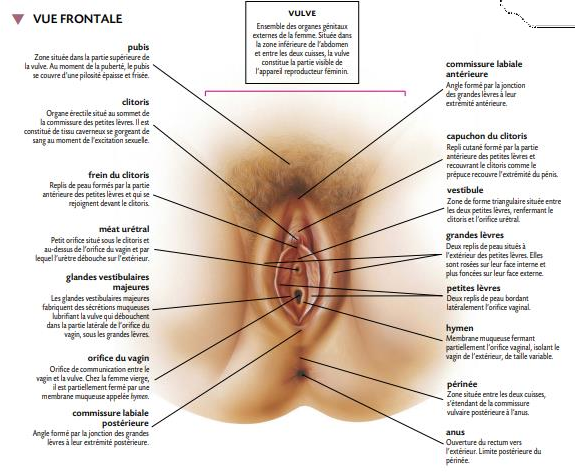
\includegraphics{Images/fig_1.png}
  \caption{Schéma montrant une vue frontale de la vulve (8)}
\end{figure}

\vspace*{1em}


\noindent Quant aux organes génitaux internes, ils résident à l'intérieur du bassin et incluent les ovaires, les trompes de Fallope, l'utérus, le col de l'utérus et le vagin. Ces organes jouent un rôle crucial dans les processus de reproduction et de régulation hormonale chez la femme. (6) \vspace*{1em}

\noindent Les ovaires se trouvent dans le pelvis et ont pour rôle principal la production de stéroïdes sexuels et la formation des ovules. Leur fonction varie selon les différentes phases du cycle menstruel. Les trompes utérines assurent le transport des gamètes et des embryons, et c'est généralement à ce niveau que la fécondation se produit. L'utérus est un organe pelvien positionné entre la vessie en avant et le rectum en arrière. Il comprend une partie dilatée appelée corps utérin, dont la partie supérieure forme le fond utérin en continuant avec le col de l'utérus, qui s'ouvre dans le vagin. Le col utérin se compose de deux parties, l'endocol et l'exocol. L'endocol contient des glandes qui sécrètent la glaire cervicale, dont sa sécrétion varie également selon les différentes phases du cycle menstruel. Le vagin, quant à lui, est un conduit musculo-membraneux constitué de trois couches : une muqueuse, une tunique et un adventice. La muqueuse vaginale subit des changements cellulaires au cours du cycle menstruel. (7) \vspace*{1em}

\begin{figure}[H]
  \centering
  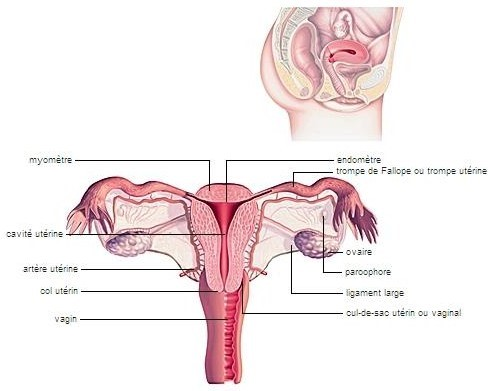
\includegraphics{Images/fig_2.jpg}
  \caption{Appareil reproducteur féminin (9)}
\end{figure}

\subsection{Rappel sur la physiologie du cycle menstruel : }

La compréhension du mécanisme d’action des différentes méthodes contraceptives nécessite une bonne connaissance de la physiologie du cycle menstruel. En effet, ce processus complexe est orchestré par le système hormonal débutant avec la libération de la gonadolibérine par l’hypothalamus. Cette hormone stimule ensuite l’hypophyse déclenchant la production des hormones folliculostimulante (FSH) et lutéinisante (LH). Ces hormones jouent un rôle crucial en influençant les ovaires à libérer des hormones sexuelles, notamment la progestérone et les œstrogènes. Ces dernières régulent divers aspects du cycle menstruel et sont essentielles à la maturation des ovules.(10) 

\begin{figure}[H]
  \centering
  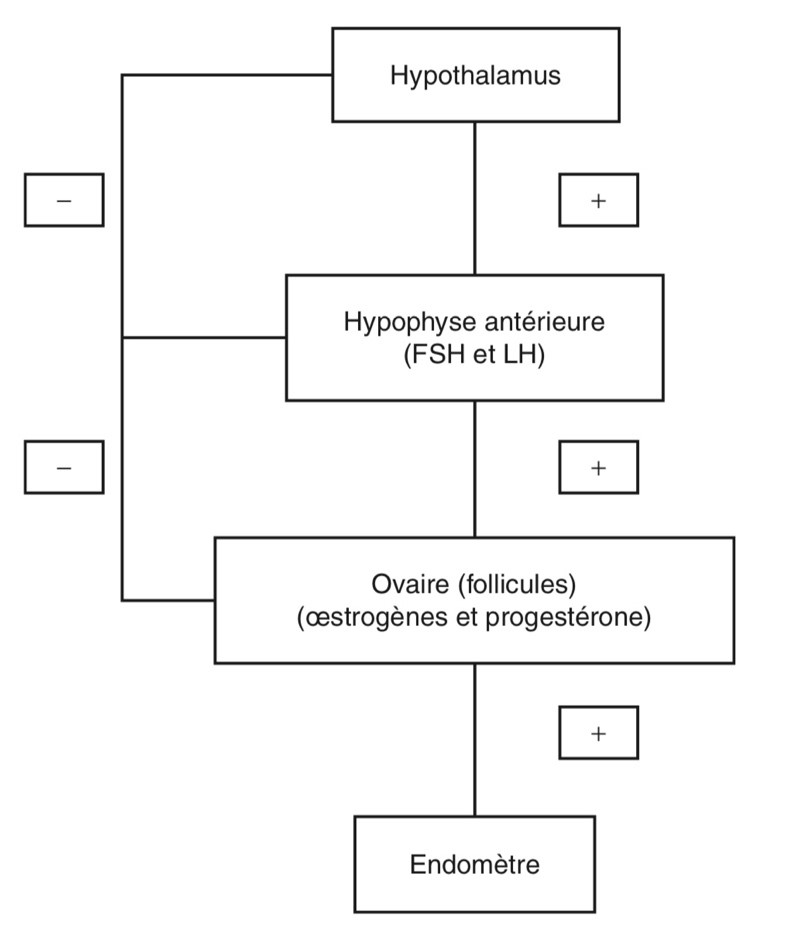
\includegraphics{Images/fig_3.jpg}
  \caption{Rétroaction biologique des hormones féminines (11)}
\end{figure}


Un cycle menstruel s'étend généralement sur une période de 28 à 32 jours, avec le premier jour marquant le début de la menstruation. (12) Ce processus naturel peut être subdivisé en quatre phases distinctes, chacune jouant un rôle spécifique dans le fonctionnement du cycle reproducteur féminin.


\hspace{1em}\textbf{•	La phase menstruelle:} \vspace{.5em}

\noindent Durant cette phase, le corps jaune, en cours de maturation, entraîne une diminution des niveaux d'hormones sexuelles, déclenchant ainsi le processus de desquamation de l'endomètre et le début des règles. Cette phase est généralement d'une durée d'environ cinq jours. 
  
\begin{figure}[H]
  \centering
  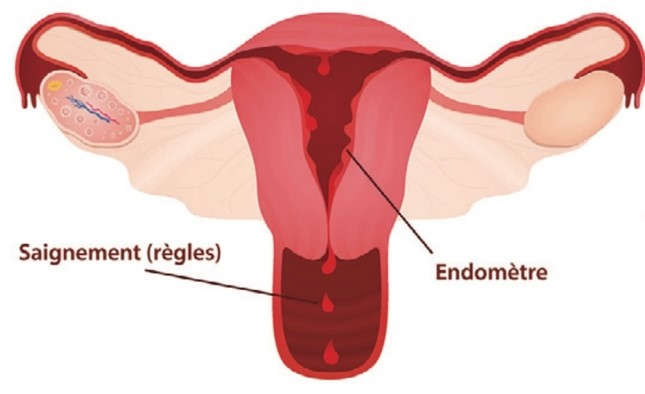
\includegraphics{Images/fig_4.jpg}
  \caption{La phase menstruelle }
\end{figure}


\hspace{1em}\textbf{•	La phase folliculaire: } \vspace{.5em}

\noindent Cette phase précède l’ovulation. La FSH stimule le développement de plusieurs follicules ovariens, cependant, un seul follicule atteint sa pleine maturité. Ce follicule contient les ovocytes qui seront ultérieurement libérés lors du processus d’ovulation.

\begin{figure}[H]
  \centering
  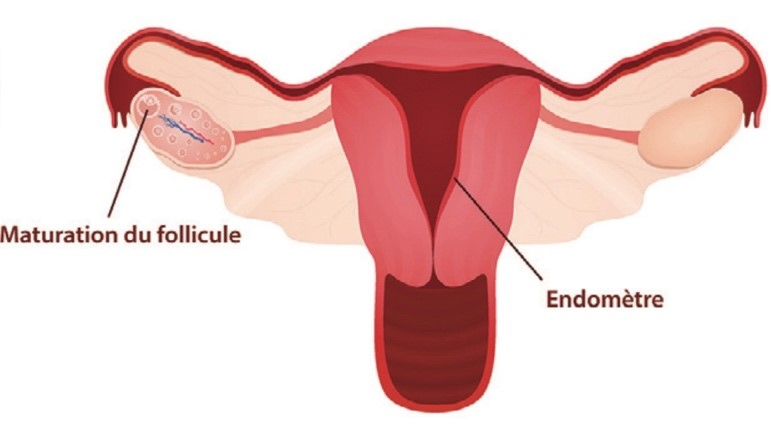
\includegraphics{Images/fig_5}
  \caption{La phase folliculaire }
\end{figure}

\hspace{1em}\textbf{•	La phase ovulatoire:  } \vspace{.5em}

\noindent Cette phase se produit généralement vers le quatorzième jour du cycle menstruel. À ce moment, la concentration élevée de l'hormone lutéinisante (LH) stimule la libération des ovocytes par le follicule ovarien mature.

\begin{figure}[H]
  \centering
  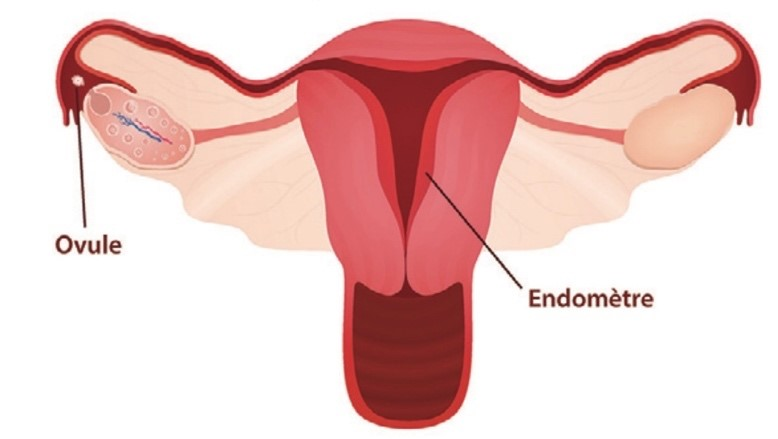
\includegraphics{Images/fig_6.jpg}
  \caption{La phase ovulatoire}
\end{figure}

\hspace{1em}\textbf{•	La phase lutéale:} \vspace{.5em}

\noindent Après l’ovulation, les niveaux de FSH et LH diminuent et le follicule rompu se transforme en corps jaune qui sécrète la progestérone et des œstrogènes. Ces hormones préparent l’endomètre à l’implantation. Si la fécondation n’a pas lieu, le corps jaune dégénère, ce qui entraîne une diminution des hormones sexuelles. Cette dégénérescence marque la fin de la phase lutéale et prépare l’organisme à l’amorce du cycle menstruel suivant.   

\begin{figure}[H]
  \centering
  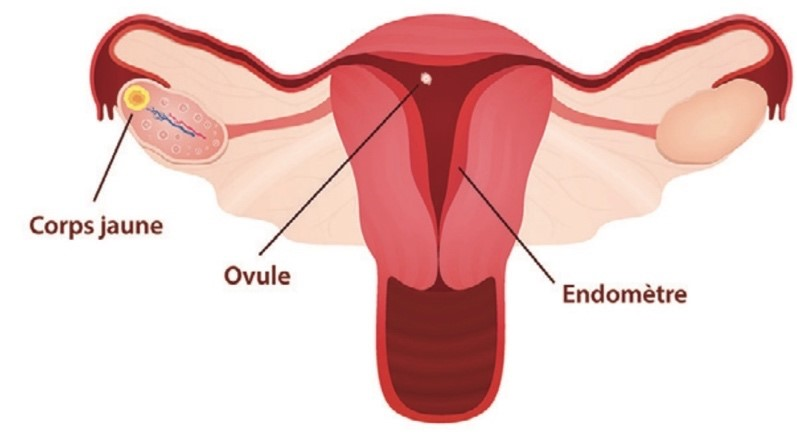
\includegraphics{Images/fig_7.jpg}
  \caption{La phase lutéale (10)}
\end{figure}

\vspace{1em}

\noindent Cette cascade complexe d'événements hormonaux constitue la base sur laquelle les méthodes contraceptives agissent. En comprenant ces mécanismes, il devient possible d'apprécier comment chaque méthode vise à perturber ou moduler ces processus, offrant ainsi une protection efficace contre les grossesse non désirées.

\begin{figure}[H]
  \centering
  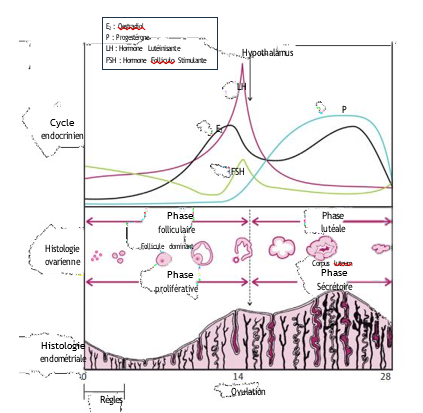
\includegraphics[scale=1.5]{Images/fig_8.jpg.png}
  \caption{Diagramme du cycle menstruel normal (13)}
\end{figure}

\subsection{Histoire de la contraception}
La pratique de la contraception remonte à des siècles, et au fil du temps, différentes méthodes ont émergé pour réguler la procréation. Certaines de ces approches historiques ont perduré jusqu'à nos jours. Voici un aperçu de quelques-unes de ces méthodes:\vspace*{1em}


\begin{itemize}[label={$\bullet$}, align=right]
  \item \textbf{La méthode du retrait:} Remontant à l'Antiquité, cette méthode consiste en l'interruption des rapports sexuels avant l'éjaculation. Bien qu'ancienne, elle est encore employée de nos jours malgré ses limitations \vspace*{0.5em}

  \item \textbf{La méthode du rythme:} Une approche basée sur le calendrier, cette méthode ancienne a évolué au fil des années. Elle repose sur la compréhension du cycle menstruel et demeure une option utilisée actuellement. \vspace*{0.5em}

  \item \textbf{La méthode Billings: }Cette méthode date des années 1960 et repose sur l'observation des sécrétions cervicales pour déterminer la période fertile de la femme. Elle est encore employée de nos jours. \vspace*{0.5em}

  \item \textbf{Les capes cervicales et les diaphragmes: }Ces dispositifs, remontant à une époque ancienne, sont toujours utilisés comme barrières contraceptives aujourd'hui, bien que des améliorations aient été apportées au fil des années.\vspace*{0.5em}

  \item \textbf{Les éponges contraceptives: }Initialement, des objets tels que des fruits ou des tissus étaient utilisés comme barrières. Les éponges, développées ultérieurement, sont toujours présentes sur le marché avec des améliorations significatives.\vspace*{0.5em}

  \begin{figure}[H]
    \centering
    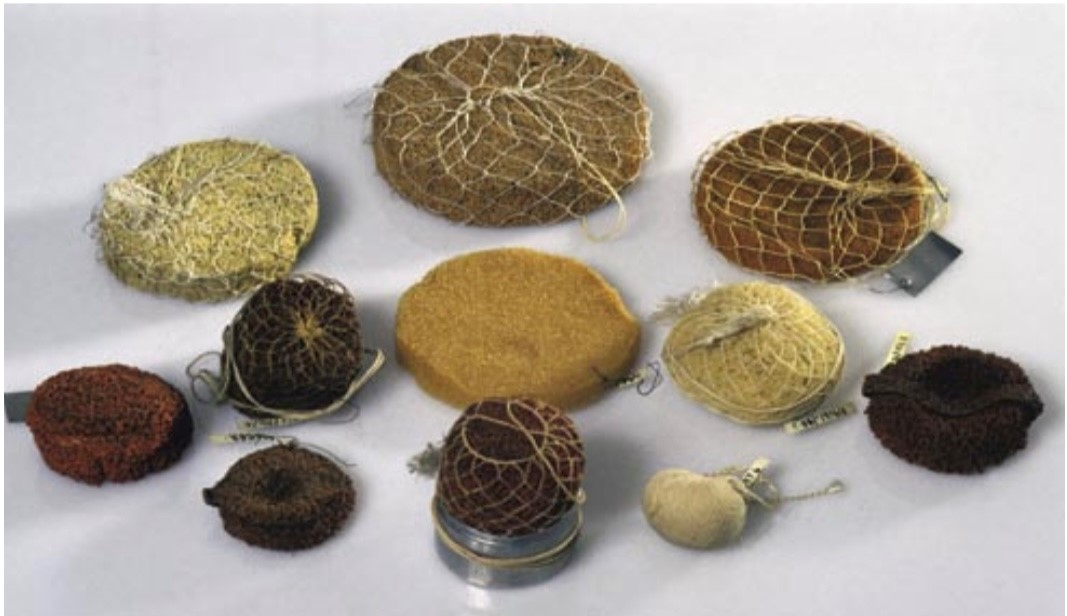
\includegraphics[scale=0.27]{Images/fig_9.jpg}
    \caption[short]{Éponges contraceptives du début du $20^e$ siècle fabriquées à partir de matériaux naturels et synthétiques.}
  \end{figure}
  
  \item \textbf{Les préservatifs: }Existants depuis des années, les préservatifs ont évolué de matériaux tels que les intestins d'animaux vers le latex et le polyuréthane modernes. Ils sont disponibles pour les deux sexes et demeurent une option populaire.


\begin{figure}[H]
    \centering
    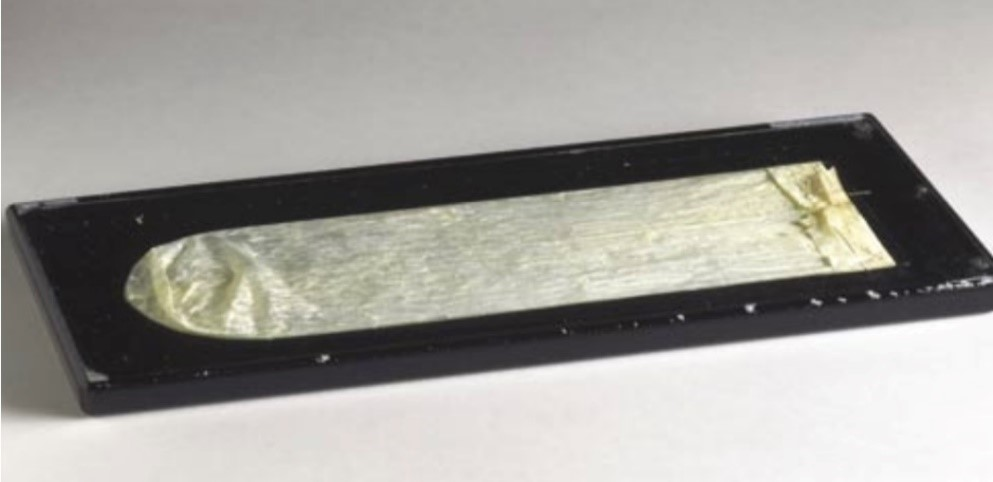
\includegraphics[scale=0.8]{Images/fig_10.jpg}
    \caption{Un préservatif masculin fait de membrane cæcale et de soie}
\end{figure}

\item \textbf{Les douches vaginales: }Utilisées autrefois pour éliminer les spermatozoïdes après les rapports, cette pratique a persisté, bien que son utilisation soit moins répandue aujourd'hui.

  \item \textbf{La contraception hormonale: }Initialement dérivées de tissus animaux, les hormones contraceptives sont désormais synthétiques. Cette méthode, largement répandue et efficace, a considérablement évolué au fil des années.

  \item \textbf{Les dispositifs intra-utérins: }Remontant à des matériaux tels que les intestins de vers à soie, les DIU modernes, notamment les stérilets, sont devenus des choix répandus et très efficaces pour la contraception.

  \item \textbf{La stérilisation: }Une méthode ancienne toujours en usage aujourd'hui, la stérilisation reste une option permanente pour ceux qui cherchent à éviter la conception.(14) 

\end{itemize}

\subsection{L’épidémiologie (statistiques démographiques): }
\noindent Entre 2015 et 2019, environ 121 millions de grossesses non désirées ont été recensées chaque année dans le monde, ce qui représente environ 48\% de l’ensemble des grossesses. Environ 61\% de ces grossesses ont été avortées. (15)\vspace*{1em}

\noindent L’Organisation des Nations Unies (ONU) estime qu’en 2050 la population mondiale se situera entre 9,4 et 10 milliards d’habitants, et la moitié des grossesses dans le monde ne sont pas désirées.(16) \vspace*{1em}

\noindent Selon Organisation Mondiale de la Santé, le nombre de femmes intéressées par la planification familiale a largement augmenté, passant de 900 millions en 2000 à environ 1,1 milliard en 2021. (17)\vspace*{1em}
  
\noindent En 2021, parmi les 1,9 milliard de femmes en âge de procréer dans le monde (15 à 49 ans), environ 1,1 milliard avaient besoin de services de planification familiales. Parmi elles, 874 millions utilisaient des méthodes de contraception modernes, tandis que 164 millions n’avaient pas accès à la contraception dont elles avaient besoin. (17)\vspace*{1em}

\noindent La proportion de femme en âge de procréer utilisant des méthodes modernes de planification familiale, est resté relativement stable à environ 77\% dans le monde entre 2015 et 2022. (17)\vspace*{1em}

\noindent En 2022, le taux global de prévalence de la contraception, toutes méthodes confondues, était estimé à 65\%, et le taux d’utilisation de méthodes contraceptives modernes par les femmes mariées ou en couple atteignait 58,7\%.(17)  \vspace*{1em}

\noindent En Afrique, en Asie et en Amérique latine, le nombre de naissances par femme était de 5 dans les années 1950, contre 2,5 aujourd’hui. L’utilisation de contraceptifs a également augmenté dans les pays en voie de développement passant de 9\% dans les années 1960 à 61\% actuellement. (18) \vspace*{1em}

\noindent Au Maroc, en 1979-1980, à peine une femme mariée sur cinq utilisait un moyen de contraception, mais en 2003-2004, plus de trois femmes mariées sur cinq y avaient recours. Entre 1962 et 2004, la fécondité a diminué progressivement, passant de 7 à 2,5 enfants par femme. (4) \vspace*{1em}

\noindent Dans les années 1960, le premier contraceptif injectable a été mis au point et c’est en 1969 que son utilisation a été approuvée. Environ 74 millions de femmes dans le monde utilisent des contraceptifs injectables en 2019, le DMPA étant le plus utilisé. (19) En Afrique subsaharienne, environ un tiers des utilisateurs de contraceptifs modernes ont recours à la contraception injectable intramusculaire. (20)\vspace*{1em}

\subsection{La stratégie nationale Marocaine dans le contrôle des naissances} 
Depuis le lancement du Programme National de Planification Familiale en 1966, des efforts considérables ont été déployés pour sensibiliser la population et répondre à ses besoins en planification familiale (PF). Plusieurs programmes ont été instaurés dans ce dessein, contribuant à élargir l'accès aux services de PF.\vspace*{1em}

\noindent Les prestation de PF sont désormais disponibles dans divers établissements de santé tels que les centres de santé, les dispensaires, les maternités, les centre de référence de PF, les cabinets médicaux et les cliniques. Une variété de professionnels de la santé, notamment des gynécologues, des chirurgiens, des médecins généralistes, et des sages - femmes, sont impliqués dans la prestation de ces services. \vspace*{1em}


\noindent Le dispositif intra-utérin, les contraceptifs oraux, les contraceptifs injectables, la contraception chirurgicale volontaire et les préservatifs figurent parmi les méthodes de PF disponibles, offrant ainsi un choix diversifié. (4) Ces méthodes sont accessibles à tous, qu'ils résident dans des zones urbaines ou rurales. (21) \vspace*{1em}  

\section{Les méthodes contraceptives }
Ce sont des méthodes naturelles ou artificielles utilisées pour prévenir une grossesse temporairement ou définitivement. Elles comprennent les méthodes naturelles, les méthodes locales, les méthodes hormonales et les méthodes chirurgicales. Cette diversité permet aux individus de choisir la méthode qui correspond le mieux à leurs besoins et à leur mode de vie.\vspace*{1em}

\subsection{Les méthodes naturelles}
Les méthodes contraceptives naturelles se distinguent par leur approche sans l'utilisation de matériel ou de produits médicaux qui interfèrent avec le système reproductif. Leur principe fondamental repose sur la compréhension et la détermination de la période de fertilité de la femme. (22) Toutefois, il est essentiel de reconnaître que ces méthodes peuvent présenter des défis, notamment lors de cycles menstruels irréguliers et chez les femmes en période péri-ménopausique, car les marqueurs d'ovulation deviennent plus difficiles à interpréter. (23)


Le retrait, également connu sous le nom de coït interrompu, se produit lorsque l'homme retire son pénis du vagin avant l'éjaculation dans le but d'éviter la fécondation.


\subsubsection{Le retrait (le coït interrompu)}
Cette méthode contraceptive est choisie par les couples désirant adopter une approche naturelle, améliorer l'efficacité d'autres méthodes contraceptives, ou encore lors de rapports sexuels occasionnels, acceptant un certain risque d'échec. Cependant, son utilisation est déconseillée dans les situations où l'homme n'est pas certain de pouvoir se retirer, en cas de risque élevé de maladies sexuellement transmissibles, et chez les femmes présentant des problèmes médicaux pour lesquelles une grossesse représente un risque important pour leur santé.\vspace*{1em}

\noindent L'efficacité du retrait repose en grande partie sur la détermination du couple à l'appliquer à chaque rapport sexuel. Les études montrent un taux d'échec estimé à 22\% dans une population donnée. Cependant, lorsque cette méthode est correctement maîtrisée par le couple, seulement 4\% des couples connaîtront une grossesse au cours des 12 mois suivants. (24)

\subsubsection{La méthode de l’allaitement maternel et de l’aménorrhée (MAMA)}
La MAMA est une option contraceptive à court terme, spécialement conçue pour les femmes récemment accouchées qui pratiquent l'allaitement exclusif. Elle peut être utilisée comme méthode contraceptive initiale avant de passer à d'autres méthodes plus durables.\\

\noindent L'efficacité de cette méthode repose sur le principe selon lequel l'allaitement fréquent inhibe la libération des hormones responsables de l'ovulation. Pour garantir une utilisation optimale, trois critères doivent être respectés:\vspace*{1em}

\begin{itemize}[label={$\bullet$}, align=right]
  \item Allaitement exclusif : La méthode MAMA fonctionne mieux lorsque la mère pratique un allaitement exclusif, sans recourir à d'autres sources de nutrition pour le nourrisson.

  \item Enfant âgé de moins de 6 mois : La méthode est recommandée jusqu'à ce que l'enfant atteigne l'âge de 6 mois. Après cette période, il est essentiel de mettre en place une autre méthode contraceptive pour maintenir une protection efficace.
  
  \item Aménorrhée chez la mère : La mère doit être aménorrhéique, c'est-à-dire ne pas avoir repris ses règles depuis l'accouchement.
  
\end{itemize}

\noindent Les études sur l'efficacité de la méthode MAMA ont révélé un taux de grossesse variant entre 0,45\% et 2,45\% à 6 mois. Des données provenant de six études non randomisées sur les utilisatrices de cette méthode ont montré un taux de grossesse allant de 0\% à 7,5\%. De plus, une étude prospective de l'Organisation Mondiale de la Santé sur l'aménorrhée de lactation et le retour de la fertilité a estimé un taux de grossesse d'environ 2\% à 6 mois. (25)

\begin{figure}[H]
  \centering
  
\includegraphics[scale=.5]{Images/fig_11.jpg}
  \caption{La méthode de l’allaitement maternel et de l’aménorrhée (26)}
\end{figure}

\subsubsection{La méthode du calendrier }
La méthode du calendrier, également connue sous le nom de méthode Ogino-Knauss, a été élaborée dans les années 1920 par Kyusaku Ogino et Herman Knaus. Elle propose une approche simple, demandant aux femmes de surveiller la durée de leur cycle menstruel afin de déterminer leurs jours de fertilité, pendant lesquels elles doivent pratiquer l'abstinence.\\

\noindent Les jours considérés comme fertiles se situent généralement entre le 12e et le 19e jour du cycle menstruel, bien que cette plage puisse varier en fonction de la durée du cycle individuel. Il est important pour les utilisatrices de comprendre la variation potentielle en fonction de leur propre cycle. \\

\noindent Cependant, des études récentes ont mis en évidence des limitations dans l'efficacité de cette méthode. Une méta-analyse portant sur huit études a révélé un taux de 15 à 18 grossesses pour 100 utilisatrices standardisées sur une période d'observation de 12 mois. Ces résultats soulignent la nécessité pour les femmes de considérer d'autres méthodes contraceptives plus fiables. (27) \\

\begin{figure}[H]
  \begin{center}
    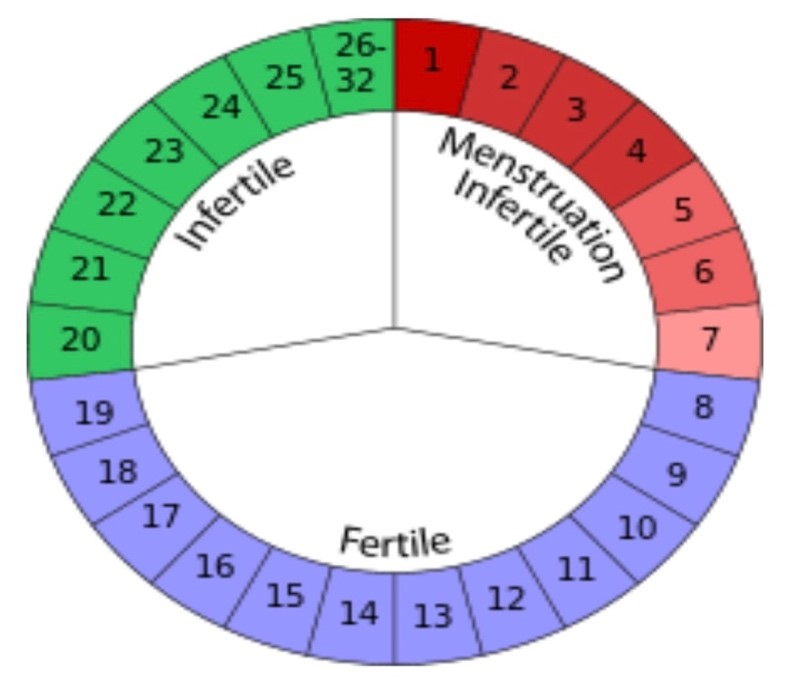
\includegraphics[scale=.8]{Images/fig_12.jpg}
    \caption{La méthode Ogino Knauss (28)}
  \end{center}
\end{figure}

\subsubsection{La méthode des deux jours}
Cette approche repose sur l'observation de la glaire cervicale pour déterminer les jours fertiles. Lorsque la glaire est présente pendant deux jours consécutifs, la fertilité est élevée. Si la glaire est présente uniquement un jour, ce jour est également considéré comme fertile. Cependant, en l'absence de glaire cervicale pendant deux jours consécutifs, la probabilité de fertilité est jugée faible. (22)\\

\subsubsection{La méthode des jours fixes}
Cette approche vise à prévenir une grossesse en évitant les rapports sexuels non protégés pendant les jours fertiles. Elle repose principalement sur l'abstinence sexuelle ou l'utilisation d'une méthode de contraception barrière, spécifiquement du 8e au 19e jour du cycle menstruel, pour les femmes dont leur cycle dure entre 26 et 32 jours. (22) 

\begin{figure}[H]
  \centering
  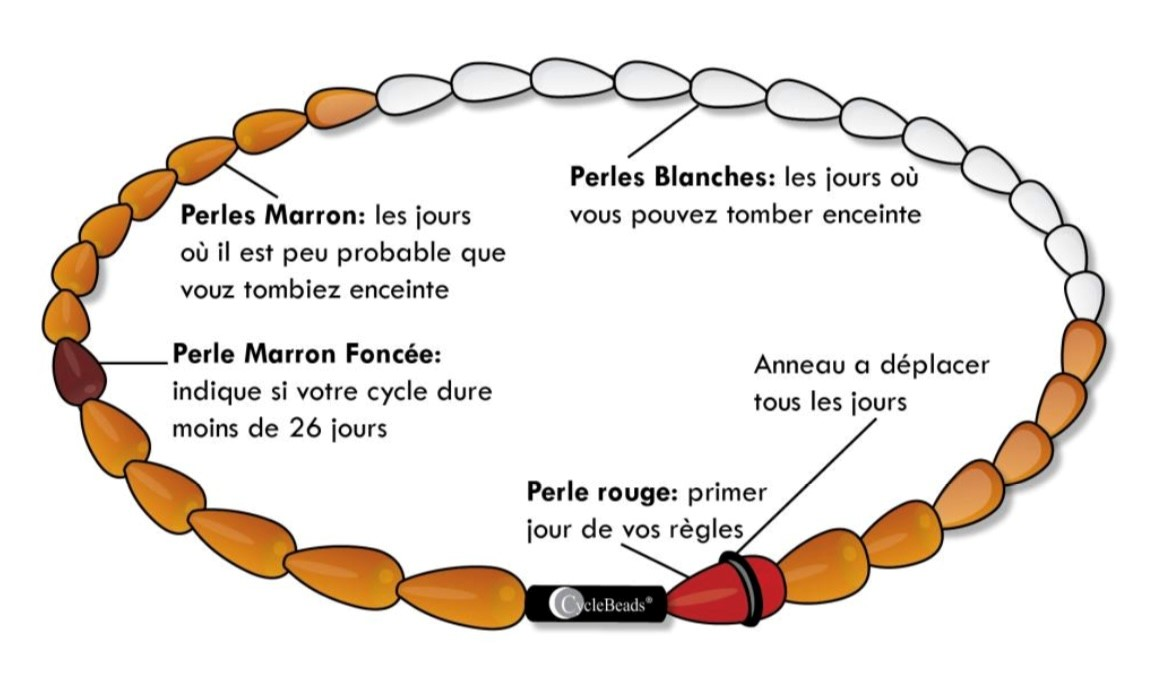
\includegraphics[scale=.3]{Images/fig_13}
  \caption{La méthode des jours fixes (29)}
\end{figure}

\subsubsection{La méthode de l’observance de la glaire cervicale}
Cette méthode, également nommée la méthode Billings, repose sur l’observation de la glaire cervicale pour permettre à la femme de déterminer sa période de fertilité. (30) \\

\noindent Il est important de noter que les rapports sexuels au cours des 5 jours précédant l'ovulation et le jour de l'ovulation présentent un risque significatif de grossesse. Pendant cette période, les sécrétions de la glaire cervicale augmentent en raison de la stimulation par l'augmentation des œstrogènes.\\

\noindent Une étude a révélé que la probabilité de conception les jours sans sécrétions est d'environ 0,3\%, tandis qu'elle est d'environ 30\% les jours où des sécrétions fertiles sont présentes. (31) 

\begin{figure}[H]
  \centering
  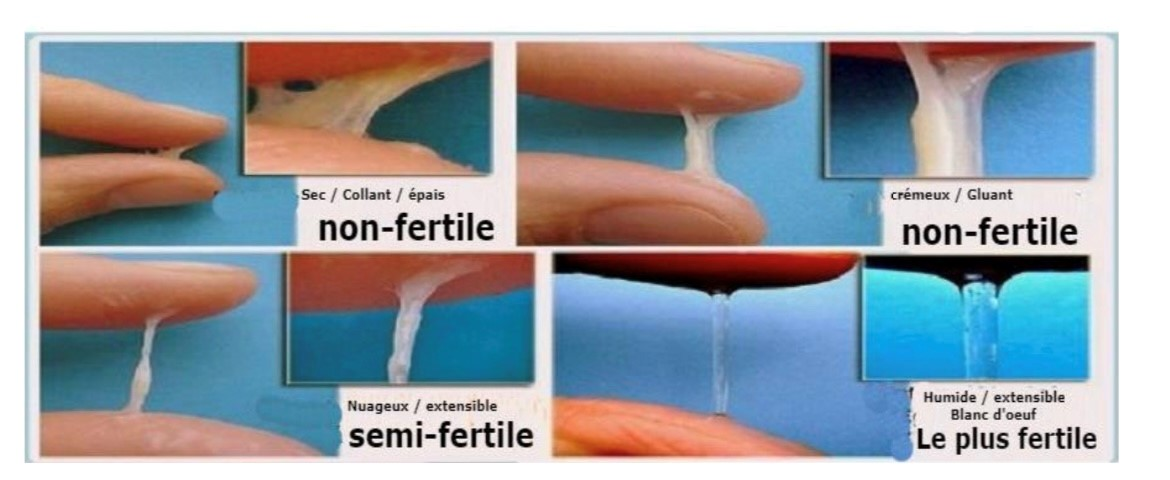
\includegraphics[scale=.3]{Images/fig_14.jpg}
  \caption{La méthode Billings (28)}
\end{figure}

\subsubsection{La méthode de la température :}
Également appelée "méthode de la température basale", cette approche implique la prise de la température corporelle au repos chaque matin, idéalement à la même heure. La méthode repose sur le principe que la température corporelle augmente après l'ovulation en raison de l'augmentation de la progestérone, signifiant la fin de la période de fertilité. Pour éviter la conception, la femme s'abstiendra de rapports sexuels pendant les trois premiers jours suivant cette augmentation de la température. (22) (32) \\

\noindent Cependant, il convient de noter que cette méthode présente des limitations en raison des influences exogènes sur la température des femmes, telles que le stress, la fièvre, et d'autres facteurs. (33)\\

\begin{figure}[H]
  \centering
  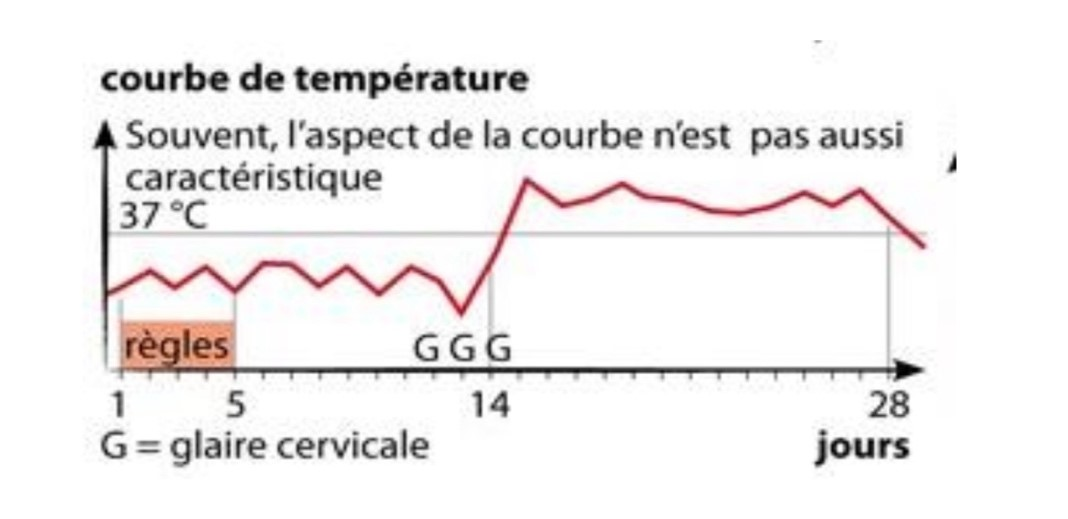
\includegraphics{Images/fig_15.jpg}
  \caption{La méthode des températures (28)}
\end{figure}

\subsubsection{La méthode symptothermique}
Il s’agit d’une méthode contraceptive qui est basée à la fois sur la méthode des températures et sur la méthode d’observation de la glaire cervicale. Les couples l'adoptent pour déterminer avec précision leur période de fertilité, en observant la température basale du corps ainsi que la texture et la quantité de la glaire cervicale. Ces informations permettent des choix éclairés pour éviter une grossesse non désirée.\\

\noindent Durant la période fertile, la température basale est notablement élevée, accompagnée d'une glaire cervicale abondante, claire, liquide et filante. En revanche, pendant la période infertile, la température basale diminue et la glaire cervicale devient plus épaisse et collante.\\

\noindent Il est intéressant de noter qu'une tendance à la hausse est observée depuis 1970 parmi les utilisatrices de cette méthode, avec une augmentation moyenne de 3 à 4\%. (34)\\ 

\begin{figure}[H]
  \centering
  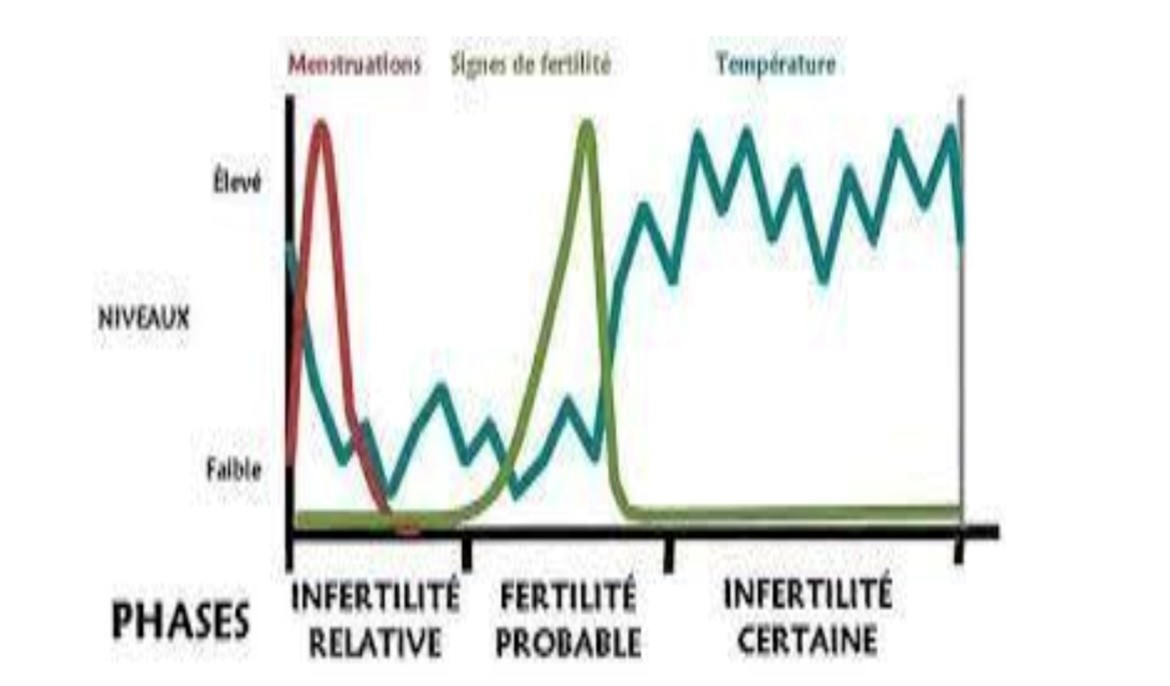
\includegraphics[scale=.3]{Images/fig_16.jpg}
  \caption{La méthode symptothermique(28)}
\end{figure}

\subsubsection{Le suivi de la fertilité utilisant des moniteurs de fertilité}
L'utilisation croissante des moniteurs de fertilité témoigne de l'intérêt grandissant des femmes pour une alternative à la contraception hormonale. Des études ont démontré que l’efficacité de cette méthode peut être aussi élevée que celle de la contraception hormonale lorsqu’elle est correctement utilisée. \\

\noindent Ces dispositifs permettent aux femmes de surveiller leur cycle menstruel en mesurant divers paramètres tels que l'augmentation de l'œstrogène dans l'urine avant l'ovulation, la présence de l'hormone lutéinisante, la température basale, etc. Cependant, il est important de noter que ces appareils peuvent être complexes à utiliser et sont parfois coûteux. (35) (36)   \\

\noindent Pendant la période de fertilité ainsi identifiée, les femmes ont le choix de s'abstenir de rapports sexuels ou d'opter pour d'autres méthodes contraceptives, telles que l'utilisation de préservatifs. \\

\begin{figure}[H]
  \centering
  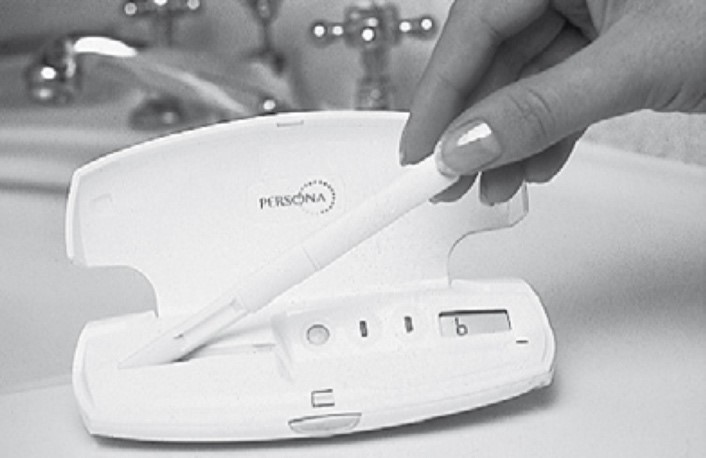
\includegraphics{Images/fig_17.jpg}
  \caption{Moniteur de fertilité (37)}
\end{figure}

\subsection{Les méthodes locales}

\subsubsection{Les préservatifs:}

\noindent Les préservatifs sont des dispositifs contraceptifs utilisés pour prévenir les grossesses en agissant comme une barrière efficace contre la pénétration du sperme. De manière notable, ils représentent également le seul moyen de contraception qui offre une protection contre les infections sexuellement transmissibles. \\

\noindent Il existe des préservatifs masculins et féminins. Ils sont généralement en latex. Toutefois, pour les individus allergiques au latex, des alternatives telles que le polyuréthane ou le nitrile, reconnus pour leur caractère hypoallergénique, sont disponibles. Ces dispositifs se déclinent dans une variété de textures, couleurs, tailles, formes, sensations et parfums. Certains sont également dotés de spermicides ou de lubrifiants.\\

\noindent Les préservatifs sont très efficaces lorsqu’ils sont utilisés correctement. Le taux d’efficacité des préservatifs masculins est de 98\% et celui des préservatifs féminins de 95\%.(38) Les couples qui utilisent le préservatif comme principal moyen de contraception ont un taux de grossesse situé entre 15 à 20\% par an. (39) 

\begin{figure}[H]
  \centering
  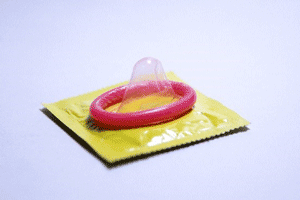
\includegraphics[scale=.7]{Images/fig_18b.jpg}
  \caption{Préservatif masculin (40)}
\end{figure}

\begin{figure}[H]
  \centering
  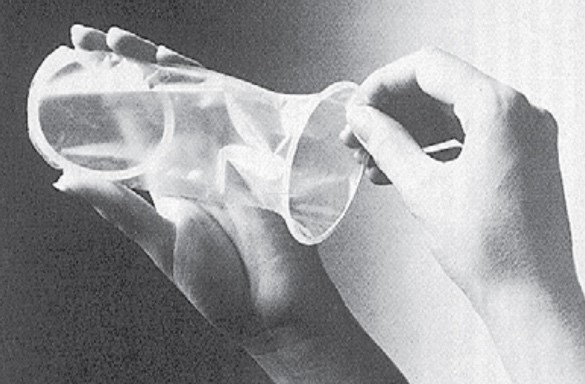
\includegraphics[scale=1]{Images/fig_19.jpg}
  \caption{Préservatif féminin (41)}
\end{figure}

\subsubsection{Les spermicides:}
\noindent Un spermicide est une méthode locale de contraception qui inactive ou tue les spermatozoïdes, empêchant ainsi la grossesse. Il est utilisé en complément d’autres méthodes contraceptives telles que les diaphragmes, les préservatifs, etc. Pour qu’il soit complètement absorbé, il doit être utilisé 10 minutes avant le rapport sexuel. Il se présente sous différentes formes galéniques (gels, crèmes, éponges, ovules, etc.). Ils peuvent être naturels ou chimiques, les deux principales molécules étant le nonoxynol-9 et le chlorure de benzalkonium. (42)\\

\noindent \textbf{Les indications des spermicides sont les suivantes :}
\begin{itemize}[label={$\bullet$}, align=right]
  \item Comme méthodes supplémentaires de contraception lors de l’utilisation :
  \begin{itemize}[label={$\circ$}]
    \item Des méthodes barrières de contraception,
    \item Des méthodes de contraception naturelles, 
    \item De contraceptifs oraux en cas d’oubli.
  \end{itemize}  

  \item Comme méthode principale de contraception chez :
  \begin{itemize}[label={$\circ$}]
    \item Les couples souhaitant seulement espacer leurs enfants,
    \item	Les femmes de plus de 45 ans,
    \item Les couples hypofertiles,
    \item Les femmes en post-partum, mais les spermicides à base de nonoxynol-9 doivent être évités pendant l’allaitement,
    \item Les couples ayant des activités sexuelles peu fréquentes,
    \item	En cas de contre-indications aux stérilets et aux pilules.  
  \end{itemize}
\end{itemize}\vspace*{1em}

\noindent \textbf{Les contre-indications des spermicides sont les suivantes :}
\begin{itemize}[label={$\bullet$}, align=right]
  \item Allergie locale aux spermicides,
  \item	Les couples qui ne veulent pas d’enfants,
  \item	Risque de contracter le VIH ou d’autres infections sexuellement transmissibles,
  \item	Les adolescentes et les jeunes femmes,
  \item	Couples sexuellement très actifs. 
\end{itemize} \vspace*{1em}

\noindent \textbf{Les avantages des spermicides sont : }
\begin{itemize}[label={$\bullet$}, align=right]
  \item Ils ne présentent pas de risque majeur pour la santé,
  \item C’est une méthode de contraception occasionnelle,
  \item Ils ne nécessitent pas de prescription médicale, 
  \item Ils donnent à la femme la possibilité de prendre en charge la contraception, 
  \item Certains spermicides ont des effets lubrifiants.
\end{itemize} \vspace*{1em}

\noindent \textbf{Les inconvénients des spermicides sont les suivantes :}

\begin{itemize}[label={$\bullet$}, align=right]
  \item Ils peuvent provoquer des allergies locales,  
  \item Ils ne sont pas très efficaces, 
  \item Ils doivent être utilisés à chaque rapport sexuel, 
  \item Ils sont chers,
  \item Ils nécessitent que la femme connaisse son appareil génital, 
  \item Certains spermicides ont un délai avant le début de leur efficacité,
  \item Ils sont peu acceptés, 
  \item Certains spermicides coulent excessivement. (41)
\end{itemize} \vspace*{1em}

\begin{figure}[H]
  \centering
  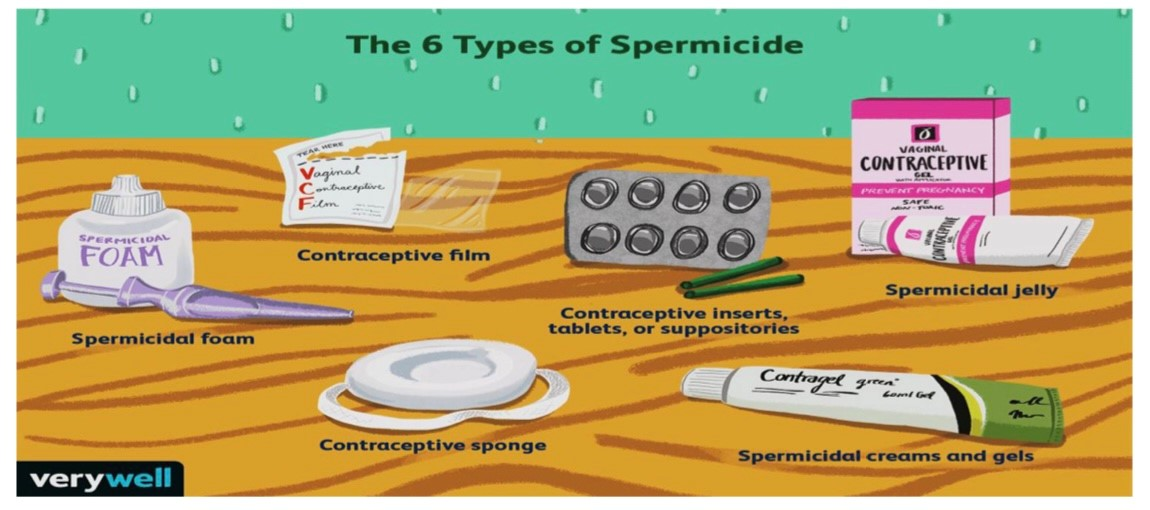
\includegraphics[scale=.4]{Images/fig_20.jpg}
  \caption{Les spermicides (40)}
\end{figure}

\noindent En France et dans d’autres pays européens, 2 à 6\% des couples utilisent des spermicides comme moyen de contraception. Pour les spermicides utilisés correctement, le taux d’échec théorique est compris entre 0 et 7,6\%. (43)  

\subsubsection{Le diaphragme :}
\noindent  C’est le premier moyen de contraception moderne fiable pour les femmes qui empêche les spermatozoïdes de traverser le col de l’utérus. (41)  Il s’agit d’un dispositif contraceptif qui peut s’avérer très efficace lorsqu’il est utilisé avec un spermicide. Il protège modérément contre les infections sexuellement transmissibles mais présente un risque d’infection des voies urinaires et de syndrome de choc toxique. (44) \\

\noindent \textbf{L’indication des diaphragmes est la suivante :}

\begin{itemize}[label={$\bullet$}, align=right]
\item  Les femmes désirant une méthode de contraception vaginale efficace et peu couteuse.
\end{itemize}\vspace*{1em}

\noindent \textbf{Les contre-indications des diaphragmes sont :}
\begin{itemize}[label={$\bullet$}, align=right]
  \item  Les femmes allergiques aux latex ou aux spermicides. 
  \item  Les femmes présentant des infections urinaires répétées. 
  \item	Anatomiques: 
  \begin{itemize}[label={$\circ$}]
    \item Périnée déficiente, 
    \item Fibrome postérieur, 
    \item Prolapsus génital important, 
    \item	Vagin plat de type juvénile, 
    \item	Rétroversion utérine fixée. 
  \end{itemize}
\end{itemize}\vspace*{1em}

\noindent \textbf{Les avantages des diaphragmes sont :}

\begin{itemize}[label={$\bullet$}, align=right]
  \item Ils peuvent être utilisés à tout âge, 
  \item	Ils préviennent modérément les infections sexuellement transmissibles,
  \item	Ils ne sont pas chers, 
  \item	Ils peuvent être placés discrètement, 
  \item Ils nécessitent un examen gynécologique, ce qui permet dépistage et suivi, 
  \item	Ils ne présentent pas de contre-indications (sauf anatomiques).
\end{itemize}\vspace*{1em}

\noindent \textbf{Les inconvénients des diaphragmes sont:}

\begin{itemize}[label={$\bullet$}, align=right]
  \item Une consultation médicale préalable est obligatoire,
  \item Les infections urinaires sont plus fréquentes chez les utilisatrices que chez les non utilisatrices,
  \item Le taux d’échec est élevé,
  \item Ils sont encombrants,
  \item Les utilisatrices nécessitent un apprentissage auprès de professionnels de la santé formés,
  \item Ils sont mal acceptés par les jeunes,
  \item Ils n’empêchent pas la transmission sexuelle du VIH. (41)  

\end{itemize}

\begin{figure}[H]
  \centering
  \begin{subfigure}[b]{0.45\textwidth}
      \centering
      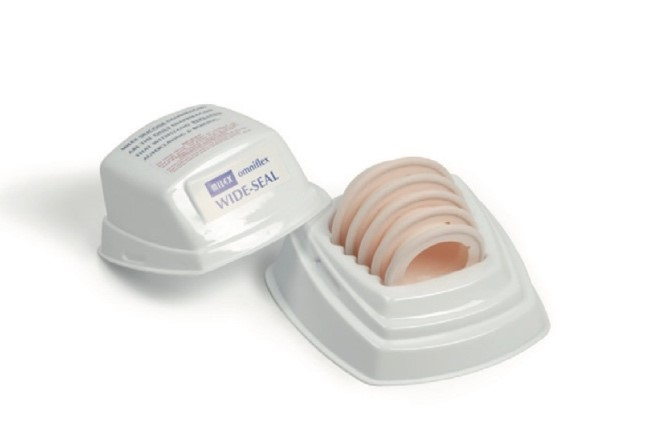
\includegraphics[width=\textwidth]{Images/fig_21a.jpg}
      % \caption{Caption for Image 1}
      % \label{fig:image1}
  \end{subfigure}
  \hfill
  \begin{subfigure}[b]{0.45\textwidth}
      \centering
      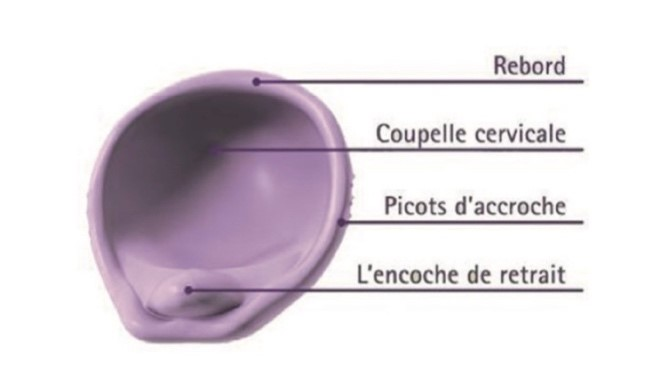
\includegraphics[width=\textwidth]{Images/fig_21b.jpg}
      % \caption{Caption for Image 2}
      % \label{fig:image2}
  \end{subfigure}
  \caption{Diaphragmes (45)}
  % \label{fig:both_images}
\end{figure}

\subsubsection{La cape cervicale :}

\noindent Elle constitue une forme de contraception féminine de type barrière. Il s’agit d’un dispositif contraceptif, une cupule en silicone ou en latex placée dans le vagin pour empêcher les spermatozoïdes d’atteindre l’ovule. Pour une meilleure efficacité, elle est utilisée avec un spermicide. Elle doit être mise en place avant le rapport sexuel et doit être laissée en place pendant au moins six heures avant de la retirer. Elle est réutilisable, mais doit être lavée avec un savon doux, séchée et conservée correctement. (22)

\begin{figure}[H]
  \centering
  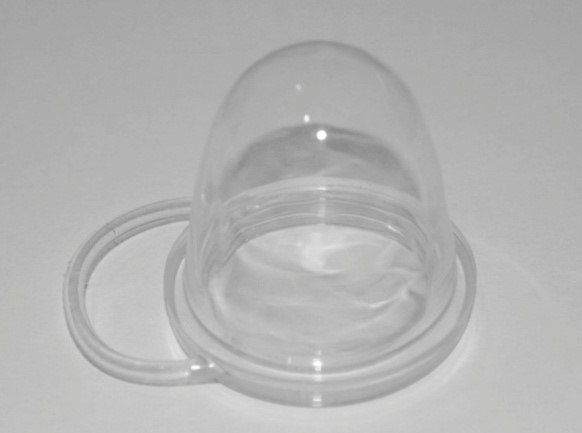
\includegraphics{Images/fig_22.jpg}
  \caption{Cape cervicale (46)}
\end{figure}

\subsubsection{L’éponge contraceptive: }
Il s’agit d’une méthode de contraception de type barrière. Elle est utilisée avec un spermicide pour être efficace. Elle recouvre le col de l’utérus et, grâce au spermicide, empêche les spermatozoïdes de pénétrer dans l’utérus.\\

\noindent \textbf{Les avantages de cette méthode sont les suivants:}

\begin{itemize}[label={$\bullet$}, align=right]
  \item	Elle est contrôlée par la femme,
  \item Elle ne contient pas d’hormones et ne présente donc pas d’effets indésirables hormonaux, 
  \item Elle ne nécessite pas de prescription médicale,
  \item	Elle ne coûte pas cher, 
  \item Il n’est pas nécessaire d’ajouter du spermicide lorsque l’éponge est réutilisée dans les 24 heures. (47)
\end{itemize}

\noindent \textbf{Les indications l’éponge contraceptive au chlorure de benzalkonium sont:}

\begin{itemize}[label={$\bullet$}, align=right]
  \item Les couples ayant des rapports sexuels peu fréquents,
  \item	Femmes de plus de 45 ans,  
  \item Contraception temporaire dans l’attente d’une contraception définitive, 
  \item Couples désirant une méthode contraceptive locale sans écoulement excessif de spermicide, 
  \item	Femmes en post-partum. 
\end{itemize}

\noindent \textbf{Les contre-indications de l’éponge contraceptive au chlorure de benzalkonium sont:}
\begin{itemize}[label={$\bullet$}, align=right]
  \item Femmes allergiques au spermicide chlorure de benzalkonium, 
  \item L’incapacité d’utiliser correctement cette méthode, 
  \item Déficience périnéale ou prolapsus génital, 
  \item Femmes sexuellement actives et fertiles. (41) 
\end{itemize}

\begin{figure}[H]
  \centering
  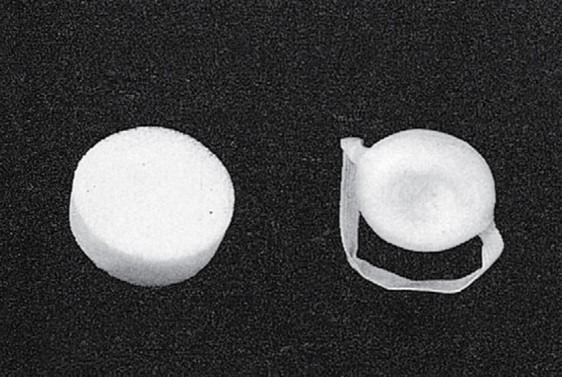
\includegraphics{Images/fig_23.jpg}
  \caption{Éponge contraceptive (41)}
\end{figure}

\subsubsection{Les dispositifs intra-utérins:}
\noindent Ils sont également connus sous le nom de stérilet et constituent le moyen de contraception le plus utilisé dans le monde. (48) Il s’agit d’une contraception à long terme, de 3 à 10 ans selon le type utilisé. Il en existe deux types, les DIU hormonaux et les DIU non hormonaux. Pour les dispositifs non hormonaux, on trouve le DIU au cuivre et pour les dispositifs hormonaux, on trouve le DIU à libération de lévonorgestrel. (49) \\

\noindent C’est un moyen de contraception très efficace avec un taux d’échec très faible de 0,3\% pour les DIU hormonaux et de 0,6 à 0,8\% pour les DIU au cuivre. (50)

\subsubsection{Les dispositifs intra-utérins hormonaux:}
\noindent Ils sont également connus sous le nom de système intra-utérin au lévonorgestrel. Leur mécanisme d’action consiste à inhiber l’ovulation et à bloquer le développement de l’endomètre. Ils inhibent également la fonction des spermatozoïdes et modifient la muqueuse endométriale pour empêcher la nidation. (10)\\

\noindent En plus de leur utilisation contraceptive, ils présentent des avantages non contraceptifs qui sont les suivants : 

\begin{itemize}[label={$\bullet$}, align=right]
  \item Ils permettent de prévenir et traiter l’hyperplasie et le cancer de l’endomètre, 
  \item	Ils aident à lutter contre l’anémie, 
  \item Ils permettent de lutter contre la ménorragie,
  \item Ils aident à traiter l’adénomyose et les fibromes, 
  \item Ils permettent de traiter l’endométriose,
  \item Ils peuvent réduire le risque de maladie inflammatoire pelvienne. (51)
\end{itemize}

\begin{figure}[H]
  \centering
  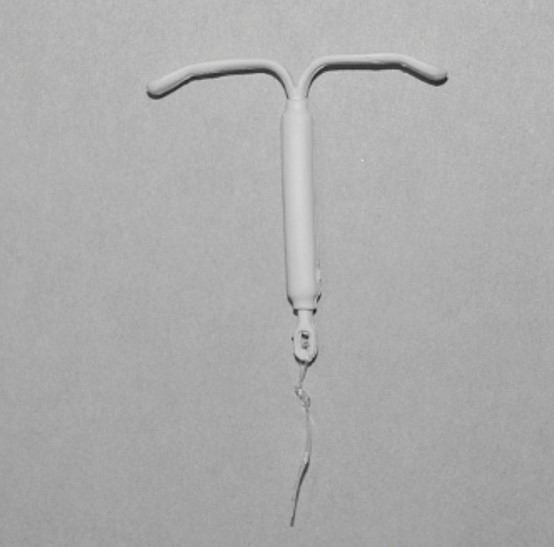
\includegraphics{Images/fig_24.jpg}
  \caption{Dispositif intra-utérin hormonal (46)}
\end{figure}

\subsubsection{Les dispositifs intra-utérins au cuivre:}

\noindent C’est une méthode de contraception non hormonale. Il s’agit d’un dispositif en plastique autour duquel est enroulé un fil de cuivre. Son mécanisme d’action est l’inhibition de l’implantation par l’effet cytotoxique du cuivre sur les spermatozoïdes. (11) Il a un effet sur la glaire cervicale empêchant la pénétration des spermatozoïdes et empêchent l’implantation par sa réponse inflammatoire sur l’endomètre. (52) 

\begin{figure}[H]
  \centering
  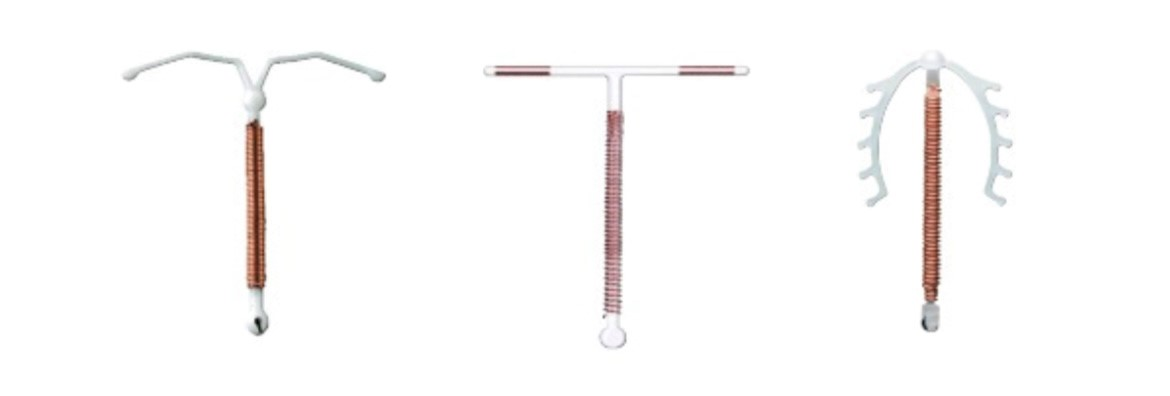
\includegraphics[scale=0.4]{Images/fig_25.jpg}
  \caption{Dispositifs intra-utérins au cuivre (53)}
\end{figure}

\noindent Cependant, bien qu’il s’agisse de l’une des méthodes de contraception les plus efficaces, elle n’est pas exempte d’inconvénients. Ces inconvénients sont notamment : 

\begin{itemize}[label={$\bullet$}, align=right]
  \item	L’expulsion du dispositif, 
  \item La douleur lors de la pose ou du retrait, 
  \item	Les ménorragies,
  \item	Les infections. (48)  
\end{itemize}

\noindent Les contre-indications absolues de cette méthode sont indiquées dans le tableau ci-dessous :

\begin{table}[H]
  \centering
  \begin{tabular}{c}
      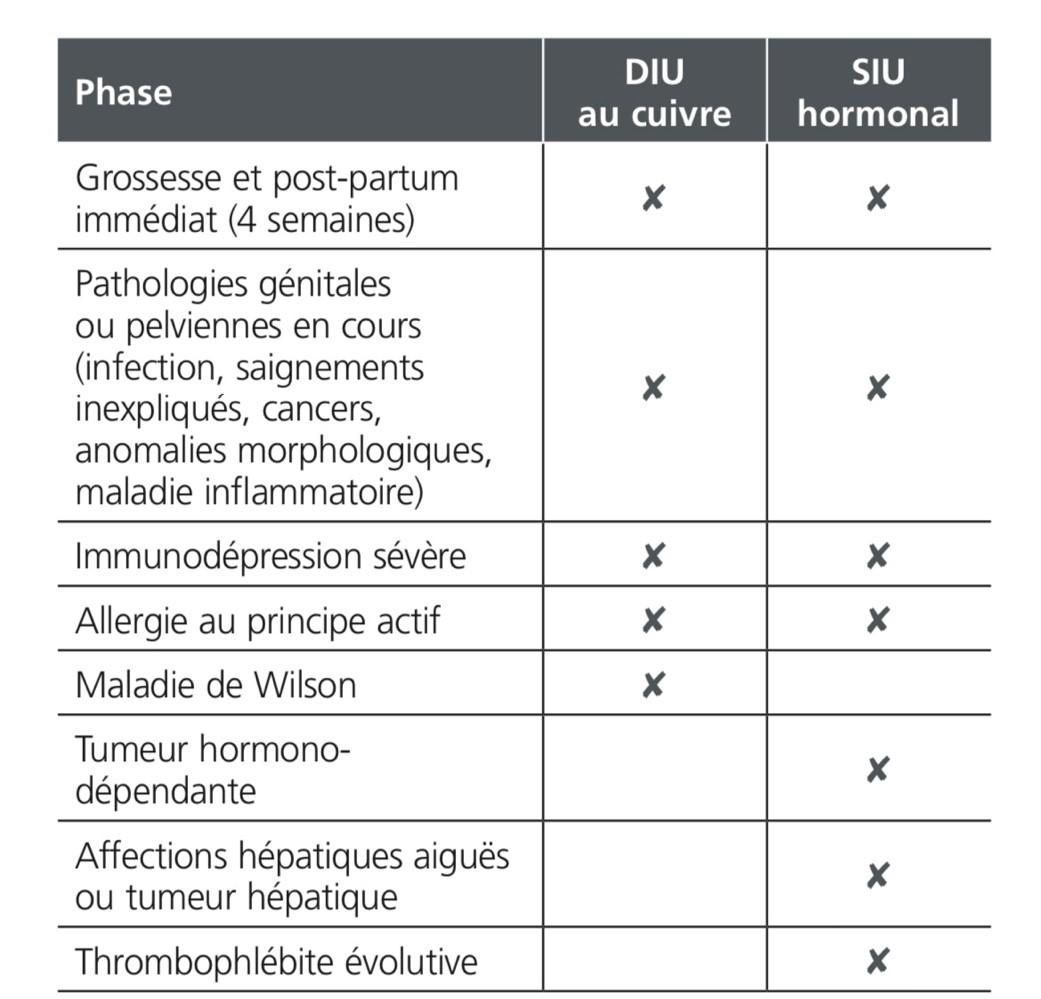
\includegraphics{Images/tab_1.jpg} \\
  \end{tabular}
  \caption{Les contre-indications absolues des dispositifs intra-utérins(53)}
  % \label{tab:contra_indications}
\end{table}

\subsection{Les méthodes hormonales:}

\noindent Les contraceptifs hormonaux sont utilisés depuis des décennies dans le monde entier pour la contraception. Ils contiennent tous un progestatif. (54) Ils agissent en inhibant l’ovulation et en modifiant la glaire cervicale, bloquant ainsi la pénétration des spermatozoïdes. (55)  Il en existe différents types comme les contraceptifs oraux, les contraceptifs injectables, les implants sous-cutanés, les stérilets, etc. Ces méthodes agissent en libérant des hormones contraceptives dans le corps.\\  

\noindent Les hormones utilisées dans la contraception hormonale sont les progestatifs et l’éthinyl estradiol.\\

\noindent \textbf{Le progestatif} est la forme synthétique de l’hormone progestérone. Ils sont utilisés pour la contraception seule ou avec l’œstrogène. Ils peuvent être classés en fonction de leur génération ou leur structure. (56)\\

\noindent Les quatre générations de progestatifs sont les suivantes : 

\begin{itemize}[label={$\bullet$}, align=right]
  \item \textbf{Première génération:} Noréthistérone
  \item \textbf{Deuxième génération:} Noréthistérone
  \item \textbf{Troisième génération:} Noréthistérone
  \item \textbf{Quatrième génération:} Drospirénone, Acétate de chlormadinone, Diénogest (10)  
\end{itemize}

\noindent D’un point de vue structurel, les progestatifs utilisés pour la contraception sont: 

\begin{itemize}[label={$\bullet$}, align=right] 
  \item Les dérivés de la testostérone tels que : 
  \begin{itemize}[label={$\circ$}]
    \item Le lévonorgestrel
    \begin{figure}[H]
      \centering
      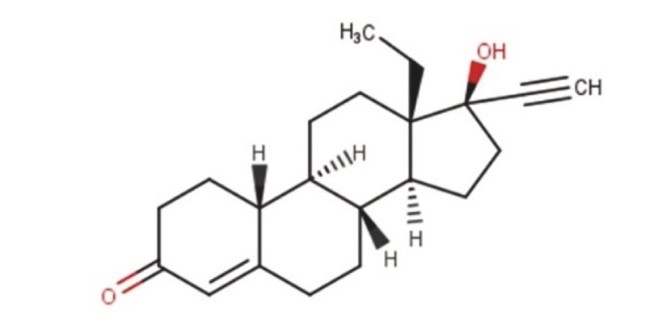
\includegraphics{Images/fig_26.jpg}
      \caption{Le lévonorgestrel (57)}
    \end{figure}
    \item La noréthistérone 
    \begin{figure}[H]
      \centering
      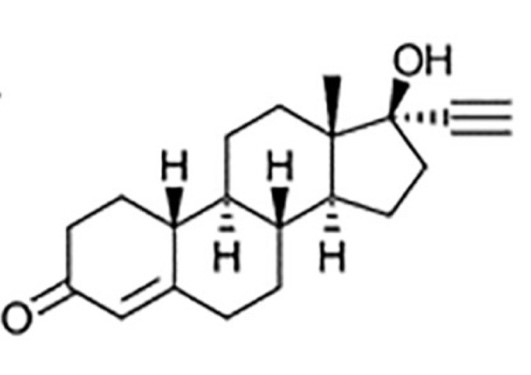
\includegraphics{Images/fig_27.jpg}
      \caption{La noréthistérone (58)}
    \end{figure}

    \item L’acétate de chlormadinone 
    \begin{figure}[H]
      \centering
      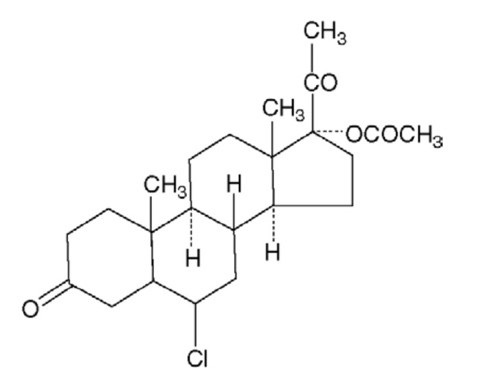
\includegraphics{Images/fig_28.jpg}
      \caption{Acétate de chlormadinone (59)}
    \end{figure}

  \end{itemize}

  \item Les dérivés du norgestrel : Ce sont des anti-gonadotropes tels que:
  \begin{itemize}[label={$\circ$}] 
    \item Norgestimate 
    \begin{figure}[H]
      \centering
      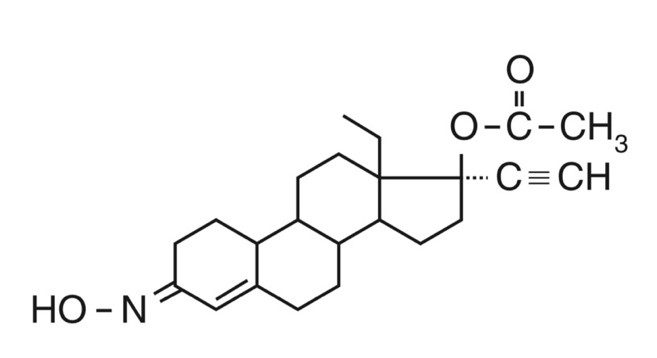
\includegraphics{Images/fig_29.jpg}
      \caption{Norgestimate (60)}
    \end{figure}
    \item Gestodène 
    \begin{figure}[H]
      \centering
      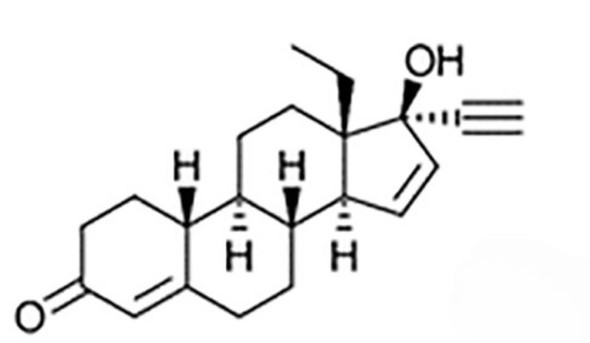
\includegraphics{Images/fig_30.jpg}
      \caption{Gestodène (58)}
    \end{figure}
    \item Désogestrel
  \end{itemize}
  \item Le dérivé de la spironolactactone : La drospirénone 
  \begin{figure}[H]
    \centering
    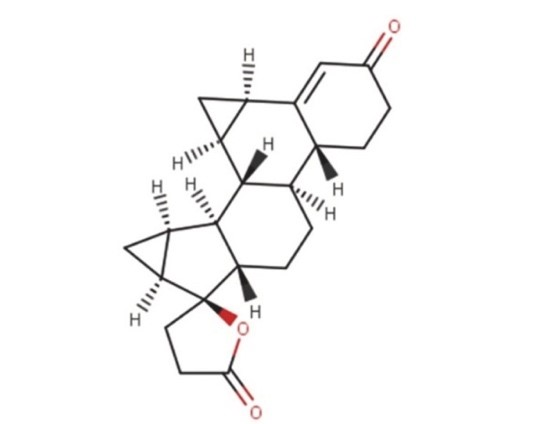
\includegraphics{Images/fig_31.jpg}
    \caption{Drospirenone (57)}
  \end{figure}

  \item Norelgestromine : C’est un précurseur du norgestrel. 
  \begin{figure}[H]
    \centering
    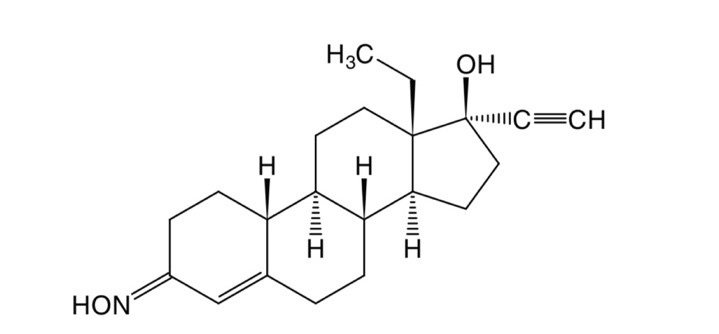
\includegraphics{Images/fig_32.jpg}
    \caption{Norelgestromine (61)}
  \end{figure}
  \item L’étonogestrel : C’est un métabolite dérivé du désogestrel. 
  \begin{figure}[H]
    \centering
    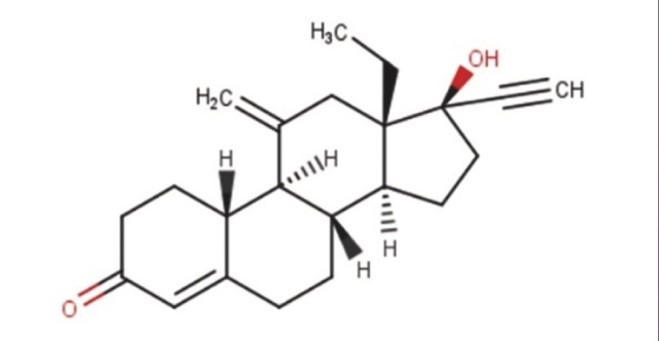
\includegraphics{Images/fig_33.jpg}
    \caption{L’étonogestrel }
  \end{figure}
  \item Le diénogest : C’est un anti-gonadotrope.  
  \begin{figure}[H]
    \centering
    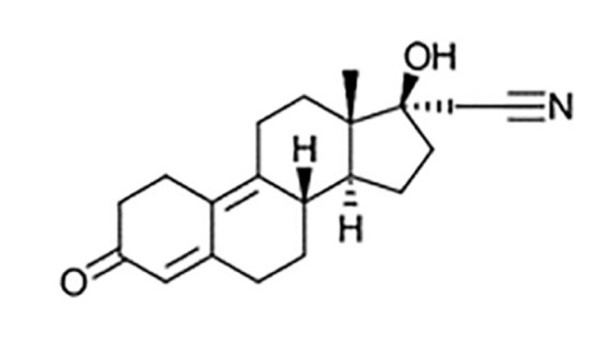
\includegraphics{Images/fig_34.jpg}    
    \caption{Le diénogest (58)}
  \end{figure}

  \item Les dérivés non stéroïdiens de la prégnane comme l’acétate de cyprotérone. (45) 
  \begin{figure}[H]
    \centering
    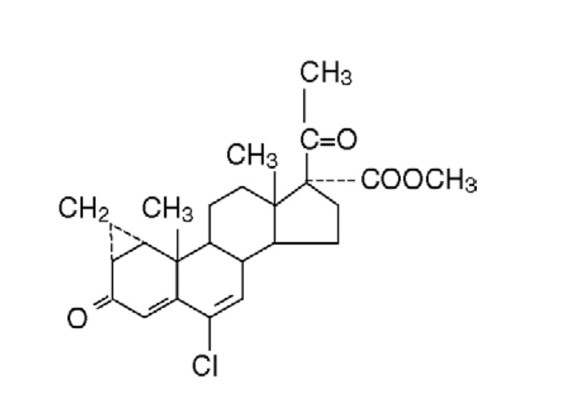
\includegraphics{Images/fig_35.jpg}
    \caption{Acétate de cyprotérone (59)}
    
  \end{figure}
  
\end{itemize}

\noindent \textbf{L’éthinylestradiol} est la forme synthétique de l’hormone œstrogène. Il s’agit de l’œstrogène le plus couramment utilisé dans la contraception. C’est un dérivé du 17$\beta$-estradiol par ajout d’un radical éthinyl en C17. (59) Il a été synthétisé pour la première fois en 1938 et c’est le premier œstrogène actif par voie orale. Il résiste à la dégradation intestinale et hépatique.  

\begin{figure}[H]
  \centering
  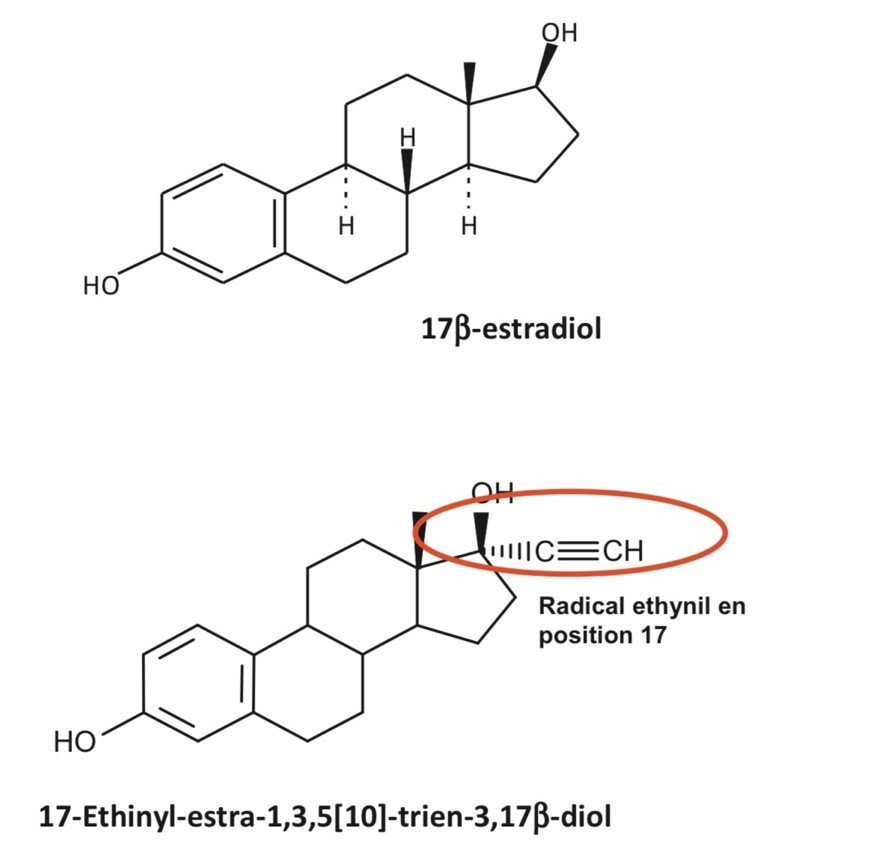
\includegraphics[scale=.6]{Images/fig_36.jpg}
  \caption{17$\beta$-estradiol et éthinylestradiol (62)}
\end{figure}

\noindent Il existe d’autres œstrogènes utilisés pour la contraception, tels que l’œstradiol, le valérate d’œstradiol, etc. (10)

\subsubsection{Les contraceptifs oraux:}

Ils sont aussi connus sous le nom de pilules contraceptives. Ces pilules peuvent être monophasiques, biphasiques ou triphasiques et se présentent en plaquette de 21 pilules ou de 28 pilules. Ce sont des hormones stéroïdiennes. Il en existe deux types, l’un composé uniquement de progestatifs également appelés contraceptifs oraux progestatifs et l’autre d’œstrogènes et de progestatifs également appelés contraceptifs oraux combinés. (2) \\

\noindent Ils sont efficaces avec un taux d’échec compris entre 7,2 et 9\%. Ces médicament sont couramment utilisés dans le cadre d’une contraception réversible et offrent des avantages non contraceptifs tels que: 

\begin{itemize}[label={$\bullet$}, align=right]
  \item	Ils réduisent les risques de certains cancers tels que le cancer de l’ovaire et de l’endomètre,
  \item	Ils régulent le cycle menstruel, aident en cas de règles irrégulières ou abondantes,
  \item Ils traitent les migraines et l’acné causées par les menstruations, 
  \item Ils traitent les troubles dysphoriques prémenstruels, 
  \item Ils aident également à soulager les crampes menstruelles, etc. (63)
\end{itemize}

\subsubsubsection{Les contraceptifs oraux progestatifs:}

Les contraceptifs à progestatifs seul présentent certains avantages: 

\begin{itemize}[label={$\bullet$}, align=right]
  \item	Les femmes qui ne peuvent pas prendre d’œstrogènes pour des raisons de santé ou autres peuvent l’utiliser,
  \item	Le mode de prise est simple,
  \item Le retour à la fertilité est presque immédiat après l’arrêt du traitement,
  \item Les fumeuses de plus de 35 ans peuvent l’utiliser, 
  \item Les femmes qui allaitent peuvent utiliser ce médicament, 
  \item Ils conviennent aux femmes qui souhaitent la dose efficace la plus faible des stéroïdes à des fins contraceptives, etc. (64)
\end{itemize}

\subsubsubsection{Les contraceptifs oraux combinés:}
Ce sont des pilules contraceptives contenant des hormones progestatives et œstrogènes. Leur mécanisme d’action est le suivant: 
\begin{itemize}[label={$\bullet$}, align=right]
  \item	L’inhibition de l’ovulation, empêchant ainsi la libération des ovules par les ovaires. C’est le principal mécanisme d’action. 
  \item Ces pilules épaississent la glaire cervicale, empêchant ainsi les spermatozoïdes de pénétrer. 
  \item	Elles bloquent aussi l’hormone lutéinisante et l’hormone folliculo-stimulante. (65)
\end{itemize}

\noindent Les COC peuvent être classés par générations en fonction de leur compositions (hormones qu’ils contiennent) et de leur évolution dans le temps. Au Maroc, les contraceptifs oraux sont classés en \textbf{quatre générations.}\vspace{2em}


\begin{table}[H]
    \centering
    \renewcommand{\arraystretch}{1.5}
    \begin{spacing}{1.5} % Set line spacing to 1.5
    \begin{tabularx}{\textwidth}{|X|p{8cm}|X|}
        \hline
        \textbf{PREMIERE \newline GENERATION} & \textbf{DOSAGE ETHINYLESTRADIOL \newline DOSAGE PROGESTATIF} & \textbf{TYPES}  \\
        \hline
        Milligynon* & Noréthistérone : 28cp à 0,6mg  &  \\
        \hline
        Triela* & Noréthistérone : 7cp à 0,5mg 
       \begin{itemize}[label={}, nosep]
        \item \hspace{21mm}7cp à 0,75mg
        \item  \hspace{20mm} 7cp à 1mg
    \end{itemize}
Ethinylestradiol : 21cp à 0,035mg 
& Triphasique \\
        \hline
    \end{tabularx}
  \end{spacing}
    \caption{Première génération de contraceptifs oraux au Maroc (66)(4)}
    %\label{tab:my_table}
\end{table}

\begin{table}[H]
  \centering
  \renewcommand{\arraystretch}{1.5}
  \begin{spacing}{1.35} % Set line spacing to 1.5
  \begin{tabularx}{\textwidth}{|X|p{8cm}|X|}
      \hline
      \textbf{DEUXIEME  \newline GENERATION} & \textbf{DOSAGE ETHINYLESTRADIOL \newline DOSAGE PROGESTATIF} & \textbf{TYPES}  \\
      \hline
      Adepal & Lévonorgestrel : 7cp à 0,15 mg
      \begin{itemize}[label={}, nosep]
        \item \hspace{20mm}14cp à 0,20mg 
    \end{itemize} 
    Ethinylestradiol : 21cp à 0,03 mg 
    \begin{itemize}[label={}, nosep]
      \item \hspace{22mm}14cp à 0,04 mg
    \end{itemize}
     & Biphasique \\
      \hline
      Microgynon* & Lévonorgestrel: 21cp à 0,15 mg 
      \newline
      Ethinylestradiol :  21cp à 0,03 mg
& Monophasique \\
\hline
Microval* & Lévonorgestrel : 28cp à 0,03mg 
&  \\  
\hline
Minidril* & Lévonorgestrel : 21cp à 0,15mg  
\newline
Ethinylestradiol : 21cp à 0,03mg 
& Monophasique \\
\hline
Stediril & Norgestrel :         21cp à 0,50mg 
\newline
Ethinylestradiol : 21cp à 0,05mg 
& Monophasique \\
\hline
Trigynon* & Lévonorgestrel : 6cp à 0,05mg  
\begin{itemize}[label={}, nosep]
  \item \hspace{22mm}5cp à 0,075mg 
  \item \hspace{22mm}10cp à 0,125mg 
\end{itemize}

Ethinylestradiol : 6cp à 0,03mg
\begin{itemize}[label={}, nosep]
  \item \hspace{22mm}5cp à 0,04mg 
  \item \hspace{22mm}10cp à 0,03mg  
\end{itemize}
& Triphasique \\
\hline
Trinordiol* & Lévonorgestrel : 6cp à 0,05mg 
\begin{itemize}[label={}, nosep]
  \item \hspace{22mm}5cp à 0,075mg  
  \item \hspace{22mm}10cp à 0,125mg  
\end{itemize} 
Ethinylestradiol : 6cp à 0,03mg
\begin{itemize}[label={}, nosep]
  \item \hspace{22mm}5cp à 0,04mg  
  \item \hspace{22mm}10cp à 0,03mg  
\end{itemize}
\vspace{1em}
& Triphasique \\
      \hline
  \end{tabularx}
\end{spacing}
  \caption{Deuxième génération de contraceptifs oraux au Maroc (66)(4)}
  %\label{tab:my_table}
\end{table}


%%%%%%%%%%%%%%%%%%%%%%%%%%%%%%%%%%%%%%%%5


\begin{table}[H]
  \centering
  \renewcommand{\arraystretch}{1.5}
  \begin{spacing}{1.35} % Set line spacing to 1.5
  \begin{tabularx}{\textwidth}{|X|p{8cm}|X|}
      \hline
      \textbf{TROISIEME   \newline GENERATION} & \textbf{DOSAGE ETHINYLESTRADIOL \newline DOSAGE PROGESTATIF} & \textbf{TYPES}  \\
      \hline
      Cerazette* & Désogestrel : 28cp à 0,075mg
     &  \\
      \hline
      Gracial* & Désogestrel : 7cp à 0,025 mg 
      \begin{itemize}[label={}, nosep]
        \item \hspace{22mm}15cp à 0,125mg
      \end{itemize}
      Ethinylestradiol : 7cp à 0,04mg
      \begin{itemize}[label={}, nosep]
        \item \hspace{22mm}15cp à 0,03mg 
      \end{itemize}
& Combiphasique \\
\hline
Mercilon* & Désogestrel : 21cp à 0,15 mg 
\newline
Ethinylestradiol : 21cp à 0,02mg
& Monophasique \\  
\hline
Microdiol* & Désogestrel : 21cp à 0,15 mg   
\newline
Ethinylestradiol : 21cp à 0,03mg  
& Monophasique \\
\hline
Minulet* &Gestodène : 21cp à 0,75mg  
\newline
Ethinylestradiol : 21cp à 0,03mg  
& Monophasique \\
\hline
Moneva* & Gestodène : 21cp à 0,75mg   
\newline
Ethinylestradiol : 21cp à 0,03mg 
& Monophasique \\
\hline
Phaeva* & Gestodène : 6cp à 0,05mg 
\begin{itemize}[label={}, nosep]
  \item \hspace{22mm}5cp à 0,07mg  
  \item \hspace{22mm}10cp à 0,07mg  
\end{itemize} 
Ethinylestradiol : 6cp à 0,03mg
\begin{itemize}[label={}, nosep]
  \item \hspace{22mm}5cp à 0,04mg   
  \item \hspace{22mm}10cp à 0,03mg   
\end{itemize}
\vspace{1em}
& Triphasique \\
      \hline
  \end{tabularx}
\end{spacing}
  \caption{Troisième génération de contraceptifs oraux au Maroc (66)(4)}
  %\label{tab:my_table}
\end{table}


\begin{table}[H]
  \centering
  \renewcommand{\arraystretch}{1.5}
  \begin{spacing}{1.5} % Set line spacing to 1.5
  \begin{tabularx}{\textwidth}{|X|p{8cm}|X|}
      \hline
      \textbf{QUATRIEME GENERATION} &  \\
      \hline
       
      Jasmine* & Drospirénone \newline Ethinylestradiol
       \\
      \hline
      Yaz* & Drospirénone \newline Ethinylestradiol
      \\
      \hline
  \end{tabularx}
\end{spacing}
  \caption{Quatrième génération de contraceptifs oraux au Maroc (66)}
  %\label{tab:my_table}
\end{table}

\noindent Bien que les COC soient généralement sûrs pour les femmes en bonne santé a faible dose, ils peuvent s’avérer dangereux pour les femmes présentant des facteurs de risques. (67)\\

\noindent \textbf{Les effets bénéfiques des COC sont présentés ci-dessous:}

\begin{table}[H]
  \centering
  \begin{tabular}{c}
      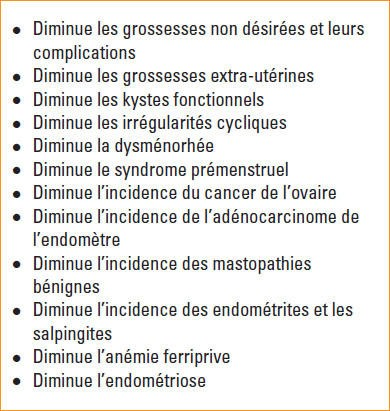
\includegraphics[scale=3.5]{Images/tab_6.jpg} \\
  \end{tabular}
  \caption{Principaux effets bénéfiques des contraceptifs oraux combinés (68)}
  % \label{tab:contra_indications}
\end{table}

\textbf{Les contre-indications des COC sont présentées ci-dessous :}

\begin{table}[H]
\centering
\begin{tabular}{c}
    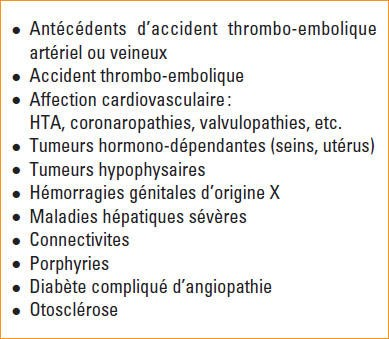
\includegraphics[scale=4.2]{Images/tab_7.jpg} \\
\end{tabular}
\caption{Contre-indications absolues des contraceptifs oraux combinés (68)}
% \label{tab:contra_indications}
\end{table}

\subsubsection{Les contraceptifs injectables:}

Les contraceptifs injectables sont des contraceptifs hormonaux administrés par voie intramusculaire (4) ou sous cutanée. Leur efficacité a été prouvée et ils sont utilisés dans de nombreux pays. Il en existe maintenant qui peuvent être auto-administrés. (69) \\

\noindent Les contraceptifs injectable peuvent être classés en deux catégories : les contraceptifs injectables à progestatif seul et les contraceptifs injectables combinés. \\

\hspace{1em}\textbf{•	Les contraceptifs injectables à progestatif seul : }\vspace*{1em}

\begin{figure}[H]
  \centering	
  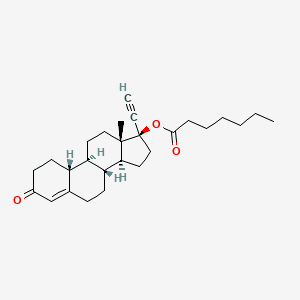
\includegraphics{Images/fig_37.jpg}
  \caption{Énanthate de noréthistérone (70)}
  
\end{figure}

\begin{figure}[H]
  \centering
  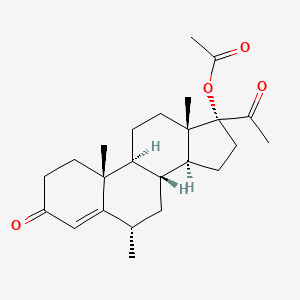
\includegraphics{Images/fig_38.png}
  \caption{Acétate de médroxyprogestérone (71)}  
\end{figure}


\begin{figure}[H]
  \centering
  \includegraphics{Images/fig_39.jpg}
  \caption{A gauche, DMPA-IM et à droite DMPA-SC (72)}
  
\end{figure}

\hspace{1em}\textbf{•	Les contraceptives injectables combinés : }\vspace*{1em}

\noindent ls contiennent de la progestérone et des œstrogènes. Ils sont administrés tous les mois. (73)

\subsubsection{Les implants sous cutanés: }
L’implant est un petit bâtonnet en plastique, inséré sous la peau à la face interne du bras, au-dessus du coude qui libère une faible dose régulière de l’hormone progestative. Il est utilisé pour la contraception à long terme car il peut assurer une couverture contraceptive pendant 3 à 5 ans. (74) \\
\noindent Le premier contraceptif implantable est le norplant* lévonorgestrel (LNG). (75) Il contenait 216mg de LNG, mais il n’est plus commercialisé. Les implants actuellement disponibles sont Implanon* etonogestrel 68mg, Jadelle* LNG 150mg, etc. Leur mécanisme d’action est l’épaississement de la glaire cervicale pour empêcher la pénétration des spermatozoïdes et l’inhibition de l’ovulation. (76)\\

\noindent Ils constituent une méthode de contraception très efficace. En plus d’être très efficaces, ils présentent certains avantages : 
\begin{itemize}
  \item Ils sont réversibles,
  \item Ils constituent une contraception de longue durée, 
  \item	L’efficacité de cette méthode ne dépend pas de l’utilisatrice
  \item Ils peuvent être utilisés par certaines personnes souffrant de complications médicales en l’absence de contre-indications. (77) 
\end{itemize}

\noindent Ces implants ont des effets indésirables tels que : 

\begin{itemize}
  \item La prise de poids, 
  \item Les troubles menstruels tels que l’aménorrhée, le spotting et les métrorragies,
  \item	Les troubles menstruels tels que l’aménorrhée, le spotting et les métrorragies,
  \item	La céphalée, 
  \item	La mastodynie, 
  \item	L’acné, etc. (78)
\end{itemize}

\begin{figure}[H]
  \centering
  \includegraphics[scale=1.2]{Images/fig_40.jpg}
  \caption{Implant sous cutané (46)}
    
\end{figure}

\subsubsection{Les contraceptifs d’urgence : }
Ils interviennent après un rapport sexuel non ou mal protégé pour éviter une grossesse. (79) Ils sont plus efficaces s’ils sont utilisés tôt. (80) In en existe deux types : les pilules contraceptives d’urgence et le stérilet en cuivre. (81)

\subsubsubsection{Les pilules hormonales contraceptives d’urgence : }
Elles sont également appelées pilules du lendemain et doivent être utilisées dans les 5 jours suivant le rapport sexuel non protégé. (80) Ces pilules ne sont pas des pilules abortives et ne peuvent pas être utilisées pour interrompre une grossesse déjà établie. Le mécanisme d’action de ces pilules est de retarder ou empêcher l’ovulation. Elles ne sont pas efficaces après l’ovulation. (82) Elles comprennent la pilule progestative contenant du LNG, la pilule anti progestative contenant de l’acétate d’ulipristal et la pilule contraceptive d’urgence combinée. Elles sont efficaces, mais certains facteurs peuvent affecter leur efficacité: 

\begin{itemize}
  \item	Les interactions médicamenteuses,
  \item	Le poids de l’utilisatrice,
  \item Le moment du rapport sexuel non protégé et de l’administration du contraceptif de la pilule, cette dernière étant plus efficace lorsqu’elle est administrée tôt,
  \item	L’ovulation : L’efficacité de la pilule diminue si elle est prise le jour de l’ovulation,
  \item	D’autres rapports sexuels non protégés après la prise de la pilule,  
  \item La malabsorption ou les vomissements. (81) 
\end{itemize}

\noindent Ces pilules ne nécessitent pas d’ordonnance, mais il est important de demander l’avis d’un professionnel de la santé avant de les utiliser. Elles empêchent l’ovulation, la fécondation ou l’implantation de l’ovule fécondé. Elles ne doivent pas être utilisées de manière systématique, mais uniquement en cas d’urgence, par exemple : 

\begin{itemize}
  \item En cas d’oubli de pilules contraceptives orales, 
  \item En cas de retard de réinjection des contraceptifs injectables, 
  \item En cas de déchirure ou de glissement du préservatif,
  \item En cas d’expulsion d’un stérilet. (83)
\end{itemize}

\vspace*{1em}

\noindent\textbf{Les avantages de la contraception d’urgences sont: }

\begin{itemize}
  \item Elle ne présente d’effets indésirables à long terme,
  \item Son taux d’échec est faible, 
  \item Elle peut être obtenue facilement de santé, 
  \item	Elle peut être prise jusqu’à 72 heures après un rapport sexuel non protégé,
  \item	La pilule est facile à prendre, 
  \item Elle présente moins d’effets secondaires par rapport à d’autres contraceptifs hormonaux combinés. 
\end{itemize}

\vspace*{1em}

\noindent\textbf{Les inconvénients de la contraception d’urgence sont: }

\begin{itemize}
  \item	Elle peut perturber le cycle menstruel, 
  \item Elle est inefficace si elle est prise après 72 à 120 heures après un rapport sexuel non protégé, 
  \item Elle ne protège pas contre les infections sexuellement transmissibles,
  \item Elle peut provoquer des nausées et des vomissements. (84)
\end{itemize}

\subsubsubsection{Les dispositifs intra-utérins: }
Le stérilet en cuivre a un effet contraceptif d’urgence s’il est utilisé dans les 5 à 7 jours suivant un rapport sexuel non protégé. (80) Ce sont les contraceptives d’urgences les plus efficaces, avec un taux de réussite de plus de 99\%. Ils peuvent être utilisés même après l’ovulation. Les ions Cu2+ affectent la fonction des spermatozoïdes et empêchent ainsi la fécondation. (81) 

\subsubsection{Le patch contraceptif: }

Ce contraceptif hormonal se porte sur la peau. Il s’agit d’un contraceptif hormonal combiné contenant de la progestérone et de l’œstrogène qui sont libérés dans le sang à travers la peau. Il est changé chaque semaine pendant trois semaines, puis une semaine de repos est observée. Il s’agit d’une méthode de contraception efficace. (85)   

\begin{figure}[H]
  \centering
  \includegraphics{Images/fig_41.jpg}
  \caption{Patch contraceptif (86)} 
\end{figure}

\subsubsection{L’anneau vaginal: }
Il s’agit d’un dispositif contraceptif contenant des hormones contraceptives qui sont libérées pour empêcher la grossesse en inhibant l’ovulation. Il contient une combinaison de progestérone et d’œstrogène. Il est utilisé pendant une période de trois semaines, puis retiré pour une pause d’une semaine. Il constitue une méthode de contraception très efficace. Il présente certains avantages non contraceptifs, notamment: 

\begin{itemize}
  \item	Il permet de traiter le syndrome des ovaires polykystiques, 
  \item Il est utilisé pour traiter l’endométriose, 
  \item	Il permet de traiter la dysménorrhée, 
  \item	Il permet de traiter la dysménorrhée, 
  \item	Il constitue une méthode contraceptive réversible qui permet un retour quasi immédiat à la fertilité, 
  \item	Il réduit les crampes menstruelles, 
  \item	Il aide à réguler le cycle menstruel. (87) 
\end{itemize}

\begin{figure}[H]
  \centering
  \includegraphics[scale=1.1]{Images/fig_42.jpg}
  \caption{Anneau vaginal (45)}
  
\end{figure}

\subsection{Les méthodes chirurgicales : }

Ces méthodes de contraception sont principalement utilisées par les personnes qui ne veulent plus avoir d’enfants pour des raisons médicales ou autres.

\subsubsection{La ligature des trompes de Fallope: }

La ligature des trompes de Fallope, également connue sous le nom de stérilisation féminine, est un moyen de contraception permanent pour les femmes. Elle consiste à bloquer les trompes de Fallope afin d’empêcher les ovules d’atteindre l’utérus et d’être fécondés par les spermatozoïdes. \vspace{1em}

\noindent Parmi les méthodes de stérilisation féminine, on peut citer l’interruption des trompes de Fallope par laparoscopie, la salpingectomie par laparoscopie, la stérilisation par hystéroscopie, etc. (88)

\begin{figure}[H]
  \centering
  \includegraphics{Images/fig_43.jpg}
  \caption{La ligature tubaire (89)}
\end{figure}

\subsubsection{La vasectomie: }

\noindent La vasectomie et les préservatifs sont les moyens de contraception masculine disponibles. (90) Le retrait, qui est une méthode contraceptive naturelle, peut également être utilisé, mais il est moins efficace. (91)\\

\noindent La vasectomie est une méthode de contraception permanente pour les hommes. Elle consiste à couper ou à ligaturer les canaux déférents qui achemine les spermatozoïdes du testicule à l’urèthre. Elle est très efficace. (92) Son taux d’échec est inférieur à 0,014\%. (91) Il s’agit d’une intervention chirurgicale simple, pratiquée par des urologues. \\

\noindent Les techniques de vasectomie sont les différentes méthodes qui peuvent être utilisées pour effectuer une vasectomie,  telles que la technique d’incision conventionnelle, la vasectomie sans bistouri et la vasectomie modifiée sans bistouri. Les méthodes d’occlusion vasale, c’est-à-dire les méthodes utilisées pour bloquer les canaux déférents, sont l’excision et la ligature, la cautérisation, l’interposition fasciale, la cautérisation plus l’interposition fasciale et la vasectomie ouverte. (93)

\begin{figure}[H]
  \centering
  \includegraphics{Images/fig_44.jpg}
  \caption{La vasectomie (28)}
  
\end{figure}

\section{Les particularités des contraceptifs injectables }

\noindent Les contraceptifs injectables constituent une option de contraception hormonale, pouvant être administrée soit par voie intramusculaire ou sous-cutanée. Voici quelques-unes de leur particularités :  


\subsection{Les différents types: }

Les types de contraceptifs injectables disponibles au Maroc sont le Depoprovera* (acétate de dépo-médroxy-progestérone) et le Noristerat* ou Megestron*(énantate de noréthistérone). (4) Le Depoprovera* est administré tous les trois mois et le Noristerat* tous les deux mois. 

\subsection{Composition: }

Les contraceptifs injectables progestatifs sont composés uniquement de progestérone, tandis que les contraceptifs injectables combinés sont composés de progestérone et d’œstrogène. 


\begin{table}[H]
  \centering
  \renewcommand{\arraystretch}{1.5}
  \begin{spacing}{1.5} % Set line spacing to 1.5
  \begin{tabularx}{\textwidth}{|X|p{3cm}|X|X|p{3.3cm}|X|}
      \hline
      \textbf{Principe actif} & \textbf{Nom\newline commercial} & \textbf{Charge}  & \textbf{Volume}  & \textbf{Voie d’administration} & \textbf{Durée}\\
      \hline
      DMPA & Depo-Provera*  & 150 mg & 1 mL & Intra musculaire & 3 mois\\
      \hline
      DMPA & Depo SubQ Provera 104*, Sayana*, Sayana Press*  & 104 mg & 0,65 mL & Sous cutanée  & 3 mois\\
      \hline
      NET-EN & Noristerat* & 200 mg  & 1 mL & Intra musculaire & 2 mois\\
      \hline
  \end{tabularx}
\end{spacing}
  \caption{Les différents types de contraceptifs injectables progestatifs (19)}
  %\label{tab:my_table}
\end{table}

\textbf{Les contraceptifs injectables combinés} sont administrés mensuellement par voie intramusculaire. Ils ne sont pas couramment utilisés mais les contraceptifs disponibles sont présentés dans le tableau ci-dessous : 

\begin{table}[H]
  \centering
  \renewcommand{\arraystretch}{1.5}
  \begin{spacing}{1.5} % Set line spacing to 1.5
  \begin{tabularx}{\textwidth}{|X|X|X|}
      \hline
      \textbf{Progestin } & \textbf{Estrogen} & \textbf{Nom commercial} \\
      \hline
      AMPR 25mg & Cypionate d’estradiol 5mg  & Cyclofem*\\
      \hline
      NET-EN 50mg  & Valérate d’estradiol 5mg  &  Mesigyna*\\
      \hline
      Acétophénide  \hspace{2cm} de dihyroxyprogestérone 150mg & Enanthate d’estradiol 10mg  & Deladroxate* \\
      \hline
  \end{tabularx}
\end{spacing}
  \caption{Les différents types de contraceptifs injectables combinés (94)}
  %\label{tab:my_table}
\end{table}

\subsection{Mécanisme d’action: }

Les contraceptifs injectables ont pour principal mécanisme d’action, l’inhibition de l’ovulation. (95) Cela se fait par la suppression de l’axe hypothalamique/pituaire/ovarien. (96) Les deux contraceptifs injectables disponibles au Maroc, le DMPA et le NET-EN, ont pratiquement les mêmes mécanismes d’action qui sont :  

\begin{itemize}
  \item La suppression de l’hormone folliculostimulante et de l’hormone lutéinisante pour inhiber l’ovulation 
  \item Empêcher le mouvement des spermatozoïdes dans la cavité utérine en augmentant la viscosité de la glaire cervicale
  \item Empêcher la nidation en amincissant la muqueuse endométriale. (97) 
\end{itemize}

\subsection{3.4. Indications:}

Les contraceptifs injectables progestatifs et les contraceptifs injectables combinés sont tous les deux utilisés pour la contraception de longue durée. La durée peut être d’un, deux ou trois mois selon le type de contraceptif injectable utilisé. 

\subsection{Contre-indications:}

Les contraceptifs injectables présentent certaines contre-indications : 

\begin{itemize}
  \item  Ils ne doivent pas être utilisés en cas d’hypersensibilité à l’un des composants du contraceptif,
  \item Ils ne doivent pas être utilisés en cas de saignements vaginaux non diagnostiqués, 
  \item Ils ne doivent pas être utilisés chez les femmes atteintes d’un cancer du sein,
  \item Ils ne doivent pas être utilisé pendant la grossesse. (98)
\end{itemize}

\subsection{Interactions médicamenteuses: }

Les interactions médicamenteuses peuvent être soit pharmacodynamiques, c’est-à-dire que deux médicaments ou plus interagissent et produisent des effets synergiques ou antagonistes, soit pharmacocinétiques, c’est-à-dire que l’absorption, la distribution, le métabolisme ou l’élimination d’un médicament est modifié en raison de son interaction avec d’autres médicaments, réduisant ou augmentant ainsi son effet. Ces interactions médicamenteuses peuvent altérer la sécurité et l’efficacité de médicaments. \\

\noindent Quelques interactions médicamenteuses avec les contraceptifs injectables sont les suivantes : 

\begin{itemize}[label={$\Rightarrow$}, align=right]
  \item Les inducteurs enzymatiques, qui réduisent l’effet des contraceptifs : 
  \begin{itemize}[label={$\bullet$}, nosep]
    \item Les anticonvulsivants comme la phénytoïne, la carbamazépine, le phénobarbital, etc., sont déconseillés, tandis que le rufinamide est doit être utilisé avec précaution,
    \item Les antidépresseurs comme le millepertuis sont contre-indiqués, 
    \item Les antifongiques comme la griséofulvine doit être utilisés avec précaution,
    \item Les antibiotiques comme la rifabutine et la rifampicine sont déconseillés, 
    \item Les antirétroviraux tels que l’efavirenz et l’elfitégravir, etc., doivent être utilisés avec précaution, lotanavir + ritonavir, atazanivir + ritonavir, saquinavir + ritonavir, etc., sont déconseillés
    \item Le modanafil est également déconseillé,
    \item L’aprépitant et le bosétan doivent être utilisés avec précaution. 
  \end{itemize}

  \item Les inhibiteurs enzymatiques :
  \begin{itemize}[label={$\bullet$}, nosep]    
    \item Les antifongiques azolés comme le voriconazole, le kétoconazole etc., 
    \item Les antiinflammatoires non stéroïdiens comme l’étoricoxib, 
    \item Le bocéprévir, 
    \item L’atorvastatine. (99)
  \end{itemize}
\end{itemize}


\subsection{Effets indésirables: }

Les effets indésirables des contraceptifs injectables progestatifs sont les suivants: 

\begin{itemize}[label={$\bullet$}, nosep] 
  \item Ils peuvent retarder le retour de la fertilité, 
  \item Ils peuvent provoquer des saignements irréguliers,
  \item Ils peuvent être à l’origine de changements d’humeur, voire d’une dépression. 
\end{itemize}

\vspace{1em}

\noindent Les effets indésirables communs aux contraceptifs injectables progestatifs et aux contraceptifs injectables combinés sont les suivants : 

\begin{itemize}
  \item	Ils peuvent provoquer des maux de tête, 
  \item	Ils peuvent entraîner la prise de poids, 
  \item	Ils peuvent aussi provoquer des douleurs osseuses, 
  \item	Ils peuvent provoquer une sensibilité des seins, 
  \item	Ils peuvent également causer l’aménorrhée, le spotting et la sécheresse vaginale. (100)
\end{itemize}

\subsection{Avantages et inconvénients}

\subsubsection{Avantages: }
Les contraceptifs injectables présentent généralement les avantages suivants : 

\begin{itemize}
  \item Ils permettent une contraception de longue durée, 
  \item Leur utilisation est facile,
  \item Ils sont efficaces avec un taux d’échec très faible, 
  \item Ils constituent une méthode de contraception temporaire,   
  \item	Ce moyen de contraception ne perturbe pas les rapports sexuels. 
\end{itemize}

\noindent Les avantages des contraceptifs injectables progestatifs sont les suivants : 

\begin{itemize}
  \item	Les femmes allaitantes peuvent les utiliser 6 semaines après l’accouchement, 
  \item	Les fumeuses peuvent y recourir, 
  \item	Ils ne sont pas limités à certains âges, 
  \item	Ils ne présentent pas d’effets indésirables liés à l’œstrogène, 
  \item	Les femmes souffrant de certaines maladies comme la cardiopathie valvulaire, la drépanocytose, la tuberculose, l’épilepsie, les maladies thyroïdiennes, etc., peuvent les utiliser comme moyen de contraception. (94)       
\end{itemize}

\subsubsection{Inconvénients: }

Les inconvénient des contraceptifs injectables sont les suivants: 

\begin{itemize}
  \item	Ils sont irréversibles dans la durée prescrite, 
  \item Leur effet peut durer jusqu’à 12 mois après l’injection,
  \item Leur couverture contraceptive est plus courte que celle des autres contraceptifs à long terme, 
  \item	Douleur au site d’injection. (19)
\end{itemize}

\subsection{Pharmacocinétiques :}

Le DMPA est une suspension aqueuse cristalline de 17-acétoxy-6-méthylprogestérone. Dans les 30 minutes qui suivent son injection intramusculaire, il se retrouve dans la circulation systémique et atteint son niveau d’effet contraceptif dans les 24heures. Sa concentration est maximale au cours des trois premières semaines suivant l’injection et diminue après 90 à 190 jours. Le NET-EN, quant à lui, sa concentration diminue dans les 80 à 110 jours suivant l’injection, tandis que pour le Mesigyna* et Cyclofem*, elle diminue au bout de 14 jours. (94)

\subsection{Efficacité: }

la contraception injectable est un moyen de contraception très efficace. Le DMPA, qui est un contraceptif de 3 mois, a un effet qui peut durer jusqu’à 4 mois. Ces contraceptifs ont un taux d’échec très faible. Selon certains essais cliniques, le DMPA a un taux d’échec d 0,1\% à 12 mois et de 0,4\% à 24 mois, le NET-EN, de 0,4\% à 12 mois et 0,6\% à 24 mois, le Mesigyna de 0,4\% à 12 mois et le Lunelle de 0,2\% à 12 mois. (94) 

\pagebreak



\pagebreak

\begin{itemize}
  \item[\textcolor{white}{$\Box$}] 
\end{itemize}


\vspace{7cm}

\begin{figure}[H]
  \includegraphics{Images/part_iii.png}
\end{figure}

\section*{}
\addcontentsline{toc}{section}{PARTIE II: ETUDES PRATIQUES}

\pagebreak


\setcounter{section}{0} % Restart the section counter
\section{INTRODUCTION}

Cette partie est la plus fondamentale de cette thèse. Elle est d’une grande importance car elle fournit des informations détaillées sur les protocoles et les outils déployés pour mener à bien notre étude sur l’acceptabilité de la contraception injectable au sein des établissements de santé, particulièrement du point de vue des professionnels de la santé. \\

\noindent Dans les pages qui suivent, nous détaillerons les éléments fondamentaux utilisés pour recueillir, analyser et interpréter les données issues de l’enquête menée auprès des professionnels de la santé via un questionnaire. \\    

\noindent Ces informations ont pour but de fournir une vue d’ensemble de notre démarche, ce qui permettra de suivre le cheminement qui nous a conduits aux résultats que nous allons présenter. Elles garantissent également la transparence de notre travail.

\section{METHODOLOGIE ET RESULTATS }
\subsection{Matériels}
\subsubsection{Objectifs de l’étude : }

\begin{itemize}
  \item Objectif général : \\
  L’objectif général de cette étude consiste à évaluer l’acceptabilité de la contraception injectable au sein des établissements de santé publique auprès des professionnels de santé.  
  \item Objectifs spécifiques :  
  \begin{itemize}[label={$\circ$}, nosep]
    \item Identifier les facteurs influençant l’acceptabilité de la contraception injectable. 
    \item Formuler des recommandations visant à améliorer l’acceptabilité de la contraception injectable, en prenant en compte les résultats de l’étude.  
    \end{itemize}
\end{itemize}

\subsubsection{Type d’étude : }

Il s’agit d’une étude descriptive et rétrospective. 

\subsubsection{Lieux et période de recueil des données : }

La collecte des données s'est déroulée au sein des centres de santé publique de Rabat, Salé, Kénitra et Témara, sur une période s'étalant d'août à septembre 2023.

\subsubsection{Population}

\subsubsubsection{Critères d’inclusion : }
Les critères d’inclusions étaient : 
\begin{itemize}
  \item Les professionnels de santé travaillant dans des établissements de santé publique,  
  \item Les professionnels de santé ayant des connaissances et de l’expérience dans le domaine de la contraception, en particulier la contraception injectable. 
\end{itemize}

\subsubsection{Critères de non inclusion : }
Les critères de non inclusion étaient : 

\begin{itemize}
  \item	Les professionnels de santé travaillant dans le secteur privé, 
  \item Les professionnels de santé n’ayant pas d’expérience en matière de contraception, 
  \item Les professionnels de santé ne désirant pas participer à l’étude, 
  \item Les professionnels de santé n’ayant pas répondu à la totalité des questions de l’enquête,
  \item	Les membres du grand public.
\end{itemize}

\subsection{Méthodologie }

\subsubsection{Outils de l’enquête :}

Un questionnaire créé avec l’outil Google Forms.

\subsubsection{Méthode de recueil des données :}
L’ensemble des données a été recueilli par l’auto remplissage du questionnaire par les professionnels de santé eux-mêmes.   

\subsubsection{Traitement et analyse des données :}

La saisie et l’analyse des données ont été faites sur Microsoft Word et Microsoft Excel.  

\subsubsection{Méthode de recherche bibliographique : }

Les articles pertinents ont été tirés de ScienceDirect, Google Scholar et PubMed pour la recherche bibliographique et le logiciel Zotero a permis de les citer.

\subsection{Résultats de l’étude : }

44 questionnaires ont étés remplis, dont 4 ont été mal remplis et 40 correctement remplis. 

\iffalse
\begin{table}[htbp]
\centering
\renewcommand{\arraystretch}{1.5}
  \begin{spacing}{1.5}
\arrayrulecolor{blue} % Set the color of the border lines to blue
\begin{tabular}{|>{\bfseries}l|l|l|}
    \hline
    \rowcolor{blue!20} % Set the background color of the first row to blue!20
    \textcolor{Statuts professionnel } & \textcolor{Effectif} & \textcolor{Pourcentage} \\
    \hline(x, y)
    Infirmier & 9 & 22,50\% \\
    \hline
    Sage-femme & 14 & 35\% \\
    \hline
    Médecin & 17 & 42,50\% \\
    \hline
    Total & 40 & 100\% \\
    \hline
\end{tabular}
\end{spacing}
\caption{Example table with blue border lines and a blue background in the first row}
\label{tab:blue_border_lines}
\end{table}
\fi

\begin{table}[H]
  \centering
  \renewcommand{\arraystretch}{1.5}
  \arrayrulecolor{customcolor!90}
  \caption{Répartition en fonction du statut professionnel}
  \begin{spacing}{1.5} % Set line spacing to 1.5
  \begin{tabularx}{\textwidth}{|X|X|X|}
      \hline
      \rowcolor{customcolor!90}
      \textbf{\color{white}Statuts professionnel} & \textbf{\color{white}Effectif} & \textbf{\color{white}Pourcentage}  \\
      \hline
      Infirmier & 9  & 22,50\% \\
      \hline
      Sage-femme & 14 & 35\% \\
      \hline
      Médecin & 17 & 42,50\% \\
     \hline
      Total & 40 & 100\% \\
      \hline
  \end{tabularx}
\end{spacing}

  %\label{tab:my_table}
\end{table}

\noindent La majorité des participants à cette étude étaient des médecins, soit 42,50\%.  

\begin{figure}[H]
  \centering
  \includegraphics{Images/fig_45.jpg}
  \caption{La majorité des participants à cette étude étaient des médecins, soit 42,50\%. }
  
\end{figure}

\begin{table}[H]
  \centering
  \renewcommand{\arraystretch}{1.5}
  \arrayrulecolor{customcolor!90}
  \caption{Répartition en fonction du statut professionnel}
  \begin{spacing}{1.5} % Set line spacing to 1.5
  \begin{tabularx}{\textwidth}{|X|X|X|}
      \hline
      \rowcolor{customcolor!90}
      \textbf{\color{white}Lieu d’exercice} & \textbf{\color{white}Effectif} & \textbf{\color{white}Pourcentage}  \\
      \hline
      Centre de santé & 40  & 100\% \\
      \hline
      Dispensaire & 0 & 0\% \\
      \hline
      Centre mère-enfant & 0 & 0\% \\
      \hline
      Hôpital régional & 0 & 0\% \\
      \hline
      Hôpital provincial & 0 & 0\% \\
      \hline
      CHU & 0 & 0\% \\
     \hline
      Total & 40 & 100\% \\
      \hline
  \end{tabularx}
\end{spacing}

  %\label{tab:my_table}
\end{table}

\noindent Cette étude a été réalisée exclusivement dans les centres de santé. 

\begin{figure}[H]
  \centering
  \includegraphics[scale=1.2]{Images/fig_46.jpg}
  \caption{Répartition en fonction du lieu d’exercice}
  
\end{figure}

\begin{table}[H]
  \centering
  \renewcommand{\arraystretch}{1.5}
  \arrayrulecolor{customcolor!90}
  \caption{Zone d’exercice}
  \begin{spacing}{1.5} % Set line spacing to 1.5
  \begin{tabularx}{\textwidth}{|X|X|X|}
      \hline
      \rowcolor{customcolor!90}
      \textbf{\color{white}Zone d’exercice} & \textbf{\color{white}Effectif} & \textbf{\color{white}Pourcentage}  \\
      \hline
      Zone urbaine & 39 & 97,50\% \\
      \hline
      Zone rurale & 1 & 2,50\% \\
     \hline
      Total & 40 & 100\% \\
      \hline
  \end{tabularx}
\end{spacing}

  %\label{tab:my_table}
\end{table}

\noindent L’étude a été réalisée principalement dans les zones urbaines, soit 97,50\%. 

\begin{figure}[H]
  \centering
  \includegraphics{Images/fig_47.jpg}
  \caption{Zone d’exercice}  
\end{figure}

\begin{table}[H]
  \centering
  \renewcommand{\arraystretch}{1.5}
  \arrayrulecolor{customcolor!90}
  \caption{Méthodes contraceptives les plus prescrites}
  \begin{spacing}{1.5} % Set line spacing to 1.5
  \begin{tabularx}{\textwidth}{|p{8cm}|X|X|}
      \hline
      \rowcolor{customcolor!90}
      \textbf{\color{white}Méthodes contraceptives} & \textbf{\color{white}Effectif} & \textbf{\color{white}Pourcentage}  \\
      \hline
      Contraception orale & 37 & 92,50\% \\
      \hline
      Contraception orale et contraception \newline injectable & 2 & 5\% \\
      \hline
      Préservatifs  & 1 & 2,5\% \\
      \hline
      Contraception injectable & 0 & 0\% \\
     \hline
      Total & 40 & 100\% \\
      \hline
  \end{tabularx}
\end{spacing}

  %\label{tab:my_table}
\end{table}

\noindent La méthode contraceptive la prescrite est la contraception orale (92,50\%).

\begin{figure}[H]
  \centering
  \includegraphics[scale=1.23]{Images/fig_48.jpg}
  \caption{Méthodes contraceptives les plus prescrites}
\end{figure}

\begin{table}[H]
  \centering
  \renewcommand{\arraystretch}{1.5}
  \arrayrulecolor{customcolor}
  \caption{Suggestion de la contraception injectable}
  \begin{spacing}{1.5} % Set line spacing to 1.5
  \begin{tabularx}{\textwidth}{|X|X|X|}
      \hline
      \rowcolor{customcolor!90}
      \textbf{\color{white}Suggestion de la \newline contraception injectable} & \textbf{\color{white}Effectif} & \textbf{\color{white}Pourcentage}  \\
      \hline
      Oui & 33 & 82,50\% \\
      \hline
      Non & 7 & 17,50\% \\
     \hline
      Total & 40 & 100\% \\
      \hline
  \end{tabularx}
\end{spacing}

  %\label{tab:my_table}
\end{table}

\noindent La majorité des professionnels de santé, soit 82,50\%, ont proposé la contraception injectable aux femmes. 

\begin{figure}[H]
  \centering
  \includegraphics{Images/fig_49.png}
  \caption{Suggestion de la contraception injectable}
  
\end{figure}

\begin{table}[H]
  \centering
  \renewcommand{\arraystretch}{1.5}
  \arrayrulecolor{customcolor}
  \caption{Suggestion de la contraception injectable}
  \begin{spacing}{1.5} % Set line spacing to 1.5
  \begin{tabularx}{\textwidth}{|p{8cm}|X|X|}
      \hline
      \rowcolor{customcolor}
      \textbf{\color{white}Avantages de la contraception  \newline injectable} & \textbf{\color{white}Effectif} & \textbf{\color{white}Pourcentage}  \\
      \hline
      Surmonte l’oubli & 35 & 87,50\% \\
      \hline
      Longue durée de contraception & 32 & 80\% \\
      \hline
      Moins d’effets indésirables & 8 & 20\% \\
      \hline
  \end{tabularx}
\end{spacing}

  %\label{tab:my_table}
\end{table}

\noindent NB : Une personne peut donner plusieurs réponses

\vspace{2em}

\noindent Les principaux avantages de la contraception injectable selon cette étude sont de surmonter l’oubli (87,50) et d’assurer une contraception à long terme (80\%). 


\begin{figure}[H]
  \centering
  \includegraphics[scale=1.23]{Images/fig_50.png}
  \caption{Avantages de la contraception injectable}
\end{figure}

\begin{table}[H]
  \centering
  \renewcommand{\arraystretch}{1.5}
  \arrayrulecolor{customcolor}
  \caption{Inconvénients de la contraception injectable}
  \begin{spacing}{1.5} % Set line spacing to 1.5
  \begin{tabularx}{\textwidth}{|p{8cm}|X|X|}
      \hline
      \rowcolor{customcolor}
      \textbf{\color{white}Inconvénients \hspace{1cm} de \,\, la  \newline contraception injectable} & \textbf{\color{white}Effectif} & \textbf{\color{white}Pourcentage}  \\
      \hline
      Plus d’effets indésirables & 22 & 55\% \\
      \hline
      Irréversible dans la durée prescrite  & 15 & 37,50\% \\
      \hline
      Risque \,\,\, d’infection \,\, du \,\, site \newline d’administration & 6 & 15\% \\
      \hline
      Pas d’inconvénients & 3 & 7,50\% \\
      \hline
      Arthrose & 1 & 2,50\% \\
      \hline
      Pas d’inconvénients si les contre-indications sont respectées & 1 & 2,50\% \\
      \hline
  \end{tabularx}
\end{spacing}

  %\label{tab:my_table}
\end{table}

\noindent NB : Une personne peut donner plusieurs réponses

\vspace{2em}

\noindent Les principaux inconvénients de cette méthode selon l’étude sont ses effets indésirables (55\%) et son irréversibilité dans la durée prescrite (37,50\%). 

\begin{figure}[H]
  \centering
  \includegraphics[scale=1.1]{Images/fig_51.png}
  \caption{Avantages de la contraception injectable}  
\end{figure}

\begin{table}[H]
  \centering
  \renewcommand{\arraystretch}{1.5}
  \arrayrulecolor{customcolor}
  \caption{Inconvénients de la contraception injectable}
  \begin{spacing}{1.5} % Set line spacing to 1.5
  \begin{tabularx}{\textwidth}{|p{8cm}|X|X|}
      \hline
      \rowcolor{customcolor}
      \textbf{\color{white}Acceptabilité \hspace{1cm} de \,\, la  \newline contraception injection} & \textbf{\color{white}Effectif} & \textbf{\color{white}Pourcentage}  \\
      \hline
      Très acceptable & 4 & 10\% \\
      \hline
      Peu acceptable  & 31 & 77,50\% \\
      \hline
      Non acceptable & 5 & 12,5\% \\
      \hline
      Total & 40 & 100\% \\
      
      \hline
  \end{tabularx}
\end{spacing}

  %\label{tab:my_table}
\end{table}

\noindent Cette méthode contraceptive est majoritairement peu acceptable, soit 77,50\%. 

\begin{figure}[H]
  \centering
  \includegraphics[scale=1]{Images/fig_52.png}
  \caption{Acceptabilité de la contraception injectable}
   
\end{figure}

\begin{table}[H]
  \centering
  \renewcommand{\arraystretch}{1.5}
  \arrayrulecolor{customcolor}
  \caption{Inconvénients de la contraception injectable}
  \begin{spacing}{1.5} % Set line spacing to 1.5
  \begin{tabularx}{\textwidth}{|p{8cm}|X|X|}
      \hline
      \rowcolor{customcolor}
      \textbf{\color{white}Adhérence à la contraception injectable} & \textbf{\color{white}Effectif} & \textbf{\color{white}Pourcentage}  \\
      \hline
       Oui & 31 & 77,50\% \\
      \hline
      Non  & 9 & 2,50\% \\
      \hline  
      Total & 40 & 100\% \\
      
      \hline
  \end{tabularx}
\end{spacing}

  %\label{tab:my_table}
\end{table}

\noindent La plupart des utilisatrices adhère à cette méthode contraceptive, soit 77,50\%. 

\begin{figure}[H]
  \centering
  \includegraphics{Images/fig_53.png}
  \caption{Adhérence à la contraception injectable}
  
\end{figure}

\begin{table}[H]
  \centering
  \renewcommand{\arraystretch}{1.5}
  \arrayrulecolor{customcolor}
  \caption{Effets indésirables signalés par les utilisatrices}
  \begin{spacing}{1.5} % Set line spacing to 1.5
  \begin{tabularx}{\textwidth}{|p{8cm}|X|X|}
      \hline
      \rowcolor{customcolor}
      \textbf{\color{white}Effets indésirables signalés \newline par les utilisatrices} & \textbf{\color{white}Effectif} & \textbf{\color{white}Pourcentage}  \\
      \hline
      Troubles menstruels & 34 & 85\% \\
      \hline
      Prise de poids   & 23 & 57,50\% \\
      \hline
      Baisse de la libido & 6 & 15\% \\
      \hline
      Réaction au site d’injection & 6 & 15\% \\
      \hline
      Hypersensibilité mammaire & 3 & 7,50\% \\
      \hline
      Hirsutisme (la pilosité) & 2 & 5\% \\
      \hline
      Varices & 1 & 2,50\% \\
      
      \hline
  \end{tabularx}
\end{spacing}

  %\label{tab:my_table}
\end{table}

\noindent NB : Une personne peut donner plusieurs réponses

\vspace{2em}

\noindent Les principaux effets indésirables signalés par les utilisatrices sont les troubles menstruels, soit 85\% et la prise de poids, soit 57,50\%. 

\begin{figure}[H]
  \centering
  \includegraphics[scale=1.15]{Images/fig_54.png}
  \caption{Effets indésirables signalés par les patients}
  
\end{figure}

\begin{table}[H]
  \centering
  \renewcommand{\arraystretch}{1.5}
  \arrayrulecolor{customcolor}
  \caption{Cas d’échecs de la contraception injectable}
  \begin{spacing}{1.5} % Set line spacing to 1.5
  \begin{tabularx}{\textwidth}{|p{8cm}|X|X|}
      \hline
      \rowcolor{customcolor}
      \textbf{\color{white}Cas d’échec \,\, de \,\, la contraception \newline injectable} & \textbf{\color{white}Effectif} & \textbf{\color{white}Pourcentage}  \\
      \hline
      Oui & 3 & 7,50\% \\
      \hline
      Non  & 37 & 92,50\% \\
      \hline
      Total & 40 & 100\% \\
      
      \hline
  \end{tabularx}
\end{spacing}

  %\label{tab:my_table}
\end{table}

\noindent La contraception injectable est efficace avec des cas d’échec minimes, soit 7,50\%. 

\begin{figure}[H]
  \centering
  \includegraphics[scale=1.1]{Images/fig_55.png}
  \caption{Cas d’échecs de la contraception injectable}
  
\end{figure}

\begin{table}[H]
  \centering
  \renewcommand{\arraystretch}{1.5}
  \arrayrulecolor{customcolor}
  \caption{Potentielles causes d’échecs}
  \begin{spacing}{1.5} % Set line spacing to 1.5
  \begin{tabularx}{\textwidth}{|p{8cm}|X|X|}
      \hline
      \rowcolor{customcolor}
      \textbf{\color{white}Potentielles causes d’échec} & \textbf{\color{white}Effectif} & \textbf{\color{white}Pourcentage}  \\
      \hline
      Tolérance& 2 & 50\% \\
      \hline
      Non-respect du délai d’abstinence  & 1 & 25\% \\
      \hline
      Enceinte avant de prendre & 1 & 25\% \\
      
      \hline
  \end{tabularx}
\end{spacing}

  %\label{tab:my_table}
\end{table}

\begin{figure}[H]
  \centering
  \includegraphics[scale=1.1]{Images/fig_56.jpg}
  \caption{Potentielles causes d’échecs}
  
\end{figure}


\begin{table}[H]
  \centering
  \renewcommand{\arraystretch}{1.5}
  \arrayrulecolor{customcolor}
  \caption{Suivi pour les patientes}
  \begin{spacing}{1.5} % Set line spacing to 1.5
  \begin{tabularx}{\textwidth}{|p{8cm}|X|X|}
      \hline
      \rowcolor{customcolor}
      \textbf{\color{white}Suivi pour les utilisatrices \newline sous contraception injectable} & \textbf{\color{white}Effectif} & \textbf{\color{white}Pourcentage}  \\
      \hline
      Oui & 38 & 95\% \\
      \hline
      Non  & 2 & 5\% \\
      \hline
      Total & 40 & 100\% \\
      
      \hline
  \end{tabularx}
\end{spacing}

  %\label{tab:my_table}
\end{table}

\noindent La plupart des utilisatrices de cette méthode contraceptive sont suivies, soit 95\%. 

\begin{figure}[H]
  \centering
  \includegraphics[scale=1.1]{Images/fig_57.png}
  \caption{Suivi pour les utilisatrices}
  
\end{figure}


\begin{table}[H]
  \centering
  \renewcommand{\arraystretch}{1.5}
  \arrayrulecolor{customcolor}
  \caption{Degrés de satisfaction}
  \begin{spacing}{1.5} % Set line spacing to 1.5
  \begin{tabularx}{\textwidth}{|p{8cm}|X|X|}
      \hline
      \rowcolor{customcolor}
      \textbf{\color{white}Degrés de satisfaction des utilisatrices} & \textbf{\color{white}Effectif} & \textbf{\color{white}Pourcentage}  \\
      \hline
      Satisfaites & 24 & 60\% \\
      \hline
      Peu satisfaites  & 13 & 32,50\% \\
      \hline
      Non satisfaites & 3 & 7,50\% \\
      \hline
      Total & 40 & 100\% \\
      
      \hline
  \end{tabularx}
\end{spacing}

  %\label{tab:my_table}
\end{table}


\noindent Selon l’étude, plus de la moitié des utilisatrices de cette méthode contraceptive sont satisfaites, soit 60\%. 

\begin{figure}[H]
  \centering
  \includegraphics[scale=1.1]{Images/fig_58.png}
  \caption{Degrés de satisfaction}
  
\end{figure}


\section{ANALYSES ET DISCUSSIONS  }

\subsection{Population étudiée :}

L’étude a été menée auprès de différents professionnels de la santé impliqués dans la prescription et le conseil en matière de la contraception pour les femmes. Ces professionnels de santé jouent un rôle crucial en guidant les femmes dans leur choix, en expliquant les avantages, les inconvénients, les effets secondaires et en assurant leur suivi. (101) \\

\noindent La majorité de la population qui a participé à cette étude était composée de médecins (42,50\%), suivis par les sage-femmes (35\%) et les infirmiers (22,50\%). 

\subsection{Lieu d’exercice :}

\noindent L'ensemble de notre étude s'est déroulé exclusivement au sein des centres de santé, en raison de leur rôle central dans la mise en œuvre des services de planification familiale dans le secteur public.\\

\noindent Cette décision s'appuie sur les normes établies par le ministère de la Santé, comme documenté dans les standards des méthodes de planification familiale au Maroc. Selon ce document, à l'exception de la stérilisation qui doit être réalisée à l'hôpital, tous les autres moyens de contraception sont principalement accessibles au sein des centres de santé. (4) \\

\noindent Une étude réalisée en Ouganda en 2022 portant sur l’auto-injection de contraceptifs à travers la prestation régulière de services auprès des professionnels de santé dans le secteur public par Morozoff et al. a été réalisée exclusivement, soit 100\% dans les centres de santé,  ce qui valide notre conclusion soulignant ainsi que les services de contraception sont principalement obtenus dans les centres de santé. (102)\\

\noindent Notre résultat est également cohérent avec une étude menée au Mali en 2023 par DOLO M., qui a porté sur les connaissances, attitudes et pratiques des jeunes en matière de contraception moderne. Dans cette étude, les centres de santé étaient également identifiés comme le lieu privilégié d'approvisionnement en produits contraceptifs, cités par 85\% des participants. (103) \\


\begin{table}[H]
  \centering
  \renewcommand{\arraystretch}{1.5}
  \arrayrulecolor{black}

  \begin{spacing}{1.5} % Set line spacing to 1.5
  \begin{tabularx}{\textwidth}{|X|X|X|X|}
      \hline
      % \rowcolor{customcolor}
      \textbf{Lieu d’exercice} & \textbf{Notre étude } & \textbf{Morozoff et al.} & \textbf{DOLO M.} \\
      \hline
      Centre de santé & 100\% & 100\% & 85\% \\
      
      
      \hline
  \end{tabularx}
\end{spacing}
\captionsetup{justification=centering} % Center-align the caption
\caption{Comparaison de notre étude avec d’autres études sur le lieu d’exercice des \hspace{2cm} professionnels de santé}

  %\label{tab:my_table}
\end{table}

\subsection{Zone d’exercice :}

L’étude a été réalisée principalement dans les zones urbaines 97,50\% parce qu’elles étaient plus accessibles. Elle a également été réalisée dans des zones rurales, soit 2,50\%.    

\subsection{Méthodes contraceptives les plus prescrites : }

Lorsqu'il s'agit de prescrire des contraceptifs, la décision repose généralement sur le choix de l'utilisatrice ou du couple. Les divers types de contraceptifs leur sont expliqués en détail, mettant en lumière les implications de chaque option. Bien que la contraception à long terme soit encouragée, la majorité des individus préfèrent les contraceptifs oraux en raison de leur familiarité et de leur utilisation régulière.\\

\noindent Selon les résultats de notre étude, la méthode contraceptive la plus fréquemment prescrite est la contraception orale, représentant 92,50\% des cas. Pour 5\% des participants, la contraception orale et la contraception injectable sont les plus prescrites, tandis que seulement 2,50\% estiment que les préservatifs sont les plus prescrits. \\

\noindent Dans une étude approfondie portant sur l'élargissement de l’accès à la contraception au sein des communautés hawaïennes, réalisée par Baniqued et al., il a été constaté que les méthodes contraceptives les plus fréquemment prescrites étaient la pilule, le patch et l'anneau contraceptif, soit 100\%, ce qui concorde avec notre résultat. (104)

\begin{table}[H]
  \centering
  \renewcommand{\arraystretch}{1.5}
  \arrayrulecolor{black}

  \begin{spacing}{1.5} % Set line spacing to 1.5
  \begin{tabularx}{\textwidth}{|p{6cm}|X|X|}
      \hline
      % \rowcolor{customcolor}
      \textbf{Méthode les plus prescrites} & \textbf{Notre étude } & \textbf{Baniqued et al. (104)} \\
      \hline
      Contraception orale & 92,5\% & 100\%  \\
      
      
      \hline
  \end{tabularx}
\end{spacing}
\captionsetup{justification=centering} % Center-align the caption
\caption{Comparaison de notre étude à une étude similaire sur les méthodes les plus prescrites}

  %\label{tab:my_table}
\end{table}

\subsection{Suggestion de la contraception injectable : }

La vaste majorité des professionnels de la santé, soit 82,50\%, recommandent la contraception injectable aux femmes, toutefois, un pourcentage de 17,50\% ne le fait pas.\\

\noindent Parmi les raisons principales de cette réticence, l'indisponibilité occasionnelle de cette méthode occupe une place prépondérante. Un autre facteur influent réside dans le manque de familiarité avec cette option, particulièrement chez les professionnels de la santé ayant moins d’années d’expérience. \\

\noindent L'étude conduite par Laryea et al. portant sur les caractéristiques et les facteurs influençant l'utilisation des contraceptifs injectables chez les femmes de Kumasi, au Ghana, a apporté des éclairages significatifs. Selon leur conclusion, la majorité des femmes ayant recours à ces contraceptifs ont acquis des informations à ce sujet auprès de professionnels de la santé. (105) Ce résultat corrobore notre recherche, qui met également en lumière le fait que la plupart des professionnels de la santé recommandent cette méthode contraceptive aux femmes. Cette convergence de résultats renforce l'importance du rôle des professionnels de la santé dans la diffusion d'informations cruciales sur les contraceptifs injectables, soulignant ainsi l'impact positif de leur implication dans l'éducation et la sensibilisation des femmes. 

\subsection{Avantages de la contraception injectable : }

Selon notre enquête, nos participants ont souligné que la contraception injectable présente plusieurs avantages significatifs. En premier lieu, elle constitue une solution pratique pour 87,50\% des répondants, qui ont souligné qu'elle permet de surmonter l'oubli fréquent des pilules contraceptives journalières. De plus, 80\% des participants ont mis en avant le fait que la contraception injectable offre une couverture contraceptive à long terme, offrant ainsi une option plus durable et moins sujette aux erreurs humaines.\\

\noindent Selon les conclusions de l'étude réalisée par Laryea et al., plusieurs femmes utilisant la contraception injectable ont souligné son avantage qui aide à surmonter l'oubli des pilules contraceptives quotidiennes. (105) Cette constatation s'aligne avec les résultats de notre étude.\\

\noindent Une étude sur la synthèse de la recherche auprès des utilisateurs finaux pour éclairer les futures technologies de prévention à usages multiples en Afrique subsaharienne par Bhushan et al. en 2023, l’un des avantages très importants mis en évidence était sa longue durée de contraception, ce qui concorde avec notre étude. (106)\\
 
\noindent Par ailleurs, notre recherche a révélé que 20\% des participants ont mis en avant le bénéfice d'une réduction des effets indésirables associés à la contraception. Cette constatation est en corrélation avec une étude menée au Mozambique en 2016 par Jacinto et al, portant sur la sécurité et l'acceptabilité de la distribution communautaire de contraceptifs injectables. Cette recherche a démontré que 24,20\% des utilisatrices ont apprécié la contraception injectable en raison de sa moindre propension à provoquer des effets indésirables. (107) Cette observation confirme la pertinence de notre étude, où 20\% des participants ont exprimé des opinions similaires quant à la réduction des effets indésirables associés à cette méthode contraceptive. 


\begin{table}[H]
  \centering
  \renewcommand{\arraystretch}{1.5}
  \arrayrulecolor{black}

  \begin{spacing}{1.5} % Set line spacing to 1.5
  \begin{tabularx}{\textwidth}{|p{6cm}|X|X|}
      \hline
      % \rowcolor{customcolor}
      \textbf{Avantage de la contraception injectable} & \textbf{Notre étude } & \textbf{Jacinto et al (107)} \\
      \hline
      Moins d’effets indésirables & 20\% & 24.20\%  \\
      
      
      \hline
  \end{tabularx}
\end{spacing}
\captionsetup{justification=centering} % Center-align the caption
\caption{Comparaison de notre étude à une étude similaire sur les avantages de la contraception injectable}

  %\label{tab:my_table}
\end{table}

\subsection{Inconvénients de la contraception injectable :}

Quant aux inconvénients de la contraception injectable, une part significative des répondants, soit 55\%, indique qu’elle a plus d’effets indésirables, pour 37,50\%, elle est irréversible dans la durée prescrite, pour 15\% risque d’infection du site d’injection, pour 7,50\%, pas d’inconvénient, pour 2,50\%, arthrose et pour 2,50\%, pas d’inconvénient si les contre-indications sont respectées. \\

\noindent Dans les contextes spécifiques du Burkina Faso et de l'Ouganda, une étude approfondie a été menée par Callahan et al. afin d'évaluer l'intérêt potentiel des utilisatrices à l'égard des nouveaux contraceptifs à longue durée d'action. Cette recherche a souligné les inconvénients associés aux contraceptifs injectables, notamment leurs effets indésirables et leur caractère irréversible pendant la durée prescrite. (108) Cette conclusion s'aligne de manière significative avec le résultat de notre étude, mettant ainsi en lumière les deux principaux inconvénients que nous avons identifiés dans notre recherche.

\subsection{Acceptabilité de la contraception injectable : }

D'après les résultats de cette étude, la contraception injectable est peu acceptable, avec 77,50\% des participants indiquant qu'ils la considèrent comme telle. De plus, 12,50\% ont explicitement déclaré qu'elle n'était pas acceptable. En revanche, seulement 10\% ont exprimé une opinion favorable en la jugeant très acceptable.\\

\noindent Selon une étude menée par Abasiattai et al., à Uyo, au Nigéria, concernant l'utilisation de la contraception injectable DMPA, il a été constaté que seulement 15,70\% des participants ont accepté cette méthode. (109) Une étude distincte portant sur la montée et la chute de la stérilisation féminine, réalisée par Kahanshim et al. à Jos, au Nigéria, a révélé un taux d'acceptabilité de la contraception injectable de 17,90\%. Il est important de noter que ces résultats présentent une différence par rapport à ce que nous avons obtenu, et cela pourrait être attribuable à l'absence d'options comparatives dans ces études. (110) Cependant, tous ces résultats convergent vers une tendance commune, à savoir une faible acceptabilité de la contraception injectable.\\

\noindent Dans une autre étude menée à l'est de la République démocratique du Congo par Mulongo et al., portant sur l'acceptabilité de la planification familiale dans la zone de santé de Kadutu, parmi les femmes informées sur la contraception injectable (soit 62 participantes), plus de la moitié (34) ont accepté cette méthode après avoir accédé à des informations fiables sur son efficacité et ses avantages. (111)  \\

\noindent Ces résultats suggèrent que la communication joue un rôle crucial dans la perception et l'acceptabilité de la contraception injectable. Une stratégie efficace de sensibilisation et d'information sur les avantages et l'efficacité de cette méthode pourrait potentiellement accroître son acceptabilité. 

\subsection{Adhérence à la contraception injectable : }

Selon les professionnels de la santé, de nombreuses utilisatrices adhèrent à la contraception injectable. 77,50\% de nos participants, ont répondu que les utilisatrices adhéraient, mais 22,50\% ont répondu qu’elles n’adhéraient pas. \\

\noindent Pour contextualiser davantage nos résultats, examinons une étude menée en 2017 par Cover et al à Kampala, en Ouganda, sur l'auto – injection sous-cutanée de DMPA, 95\% des utilisatrices ont adhéré à cette méthode. (112) Le taux d’adhérence est plus élevé que celui de notre étude, ce qui pourrait s’expliquer par le fait que l’étude a été menée auprès des utilisatrices et non des professionnels de la santé, et qu’il pourrait donc y avoir un biais de réponse. \\

\noindent Une autre étude pertinente, réalisée au Sénégal par Cover et al en 2019 portant sur la continuité de l'auto-injection par rapport à la contraception administrée par un prestataire, a révélé un taux d’adhérence 80,2\% à la contraception injectable, ce qui correspond de près à notre résultat. (113)\\

\noindent Selon les professionnels de la santé, l'aménorrhée émerge comme la principale raison invoquée par les utilisatrices pour expliquer leur non-adhésion à la contraception injectable.

\begin{table}[H]
  \centering
  \renewcommand{\arraystretch}{1.5}
  \arrayrulecolor{black}

  \begin{spacing}{1.5} % Set line spacing to 1.5
  \begin{tabularx}{\textwidth}{|p{5cm}|X|p{3.7cm}|p{3.6cm}|}
      \hline
      % \rowcolor{customcolor}
      \textbf{L’adhérence de la \newline contraception injectable} & \textbf{Notre étude } & \textbf{Cover et al. (112)} & \textbf{Cover et al. (113)}\\
      \hline
       & 77,50\% & 95\%  & 80,20\%\\
      
      
      \hline
  \end{tabularx}
\end{spacing}
\captionsetup{justification=centering} % Center-align the caption
\caption{Comparaison de notre étude à une étude similaire sur les avantages de la contraception injectable}

  %\label{tab:my_table}
\end{table}

\subsection{Effets indésirables de la contraception injectable :}

\noindent Selon notre étude, les effets indésirables les plus fréquemment observés avec la contraception injectable comprennent en premier lieu les troubles menstruels, qui représentent 85\% des réponses recueillies. Ce problème est suivi de près par la prise de poids à 57,50\%, la baisse de la libido à 15\%, les réactions au site d'injection à 15\%, l'hypersensibilité mammaire à 7,50\%, l'hirsutisme (la pilosité) à 5\%, et les varices à 2,50\%. \\

\noindent Une étude menée en Ouganda par Hyttel et al. en 2012 sur l'utilisation des contraceptifs hormonaux injectables, en particulier le DMPA, a révélé que 90\% des utilisateurs de ce contraceptif ont signalé des troubles menstruels comme principal effet indésirable. Ce résultat est en corrélation avec notre étude, confirmant ainsi que les troubles menstruels sont les effets indésirables prédominants associés à cette méthode contraceptive. (114) \\

\noindent Une recherche similaire effectuée au Mali par N. Dao sur les effets indésirables de la contraception injectable a également identifié les troubles menstruels comme les principaux effets indésirables, soit 93,46\%. Parmi ceux-ci, les métrorragies ont été signalées par 54,06\% des participants et les aménorrhées par 39,40\%. Ces résultats concordent avec notre étude, soulignant la cohérence des conclusions dans différentes régions (115)\\

\noindent Une autre étude au Mali, réalisée par Mohamed N en 2021, se concentrant sur les raisons d'abandon des méthodes contraceptives à long terme et du Depo Provera, l'aménorrhée était l'effet indésirable le plus couramment cité, soit 95,80\%. Ces constatations sont en ligne avec nos résultats, soulignant la prévalence de l'aménorrhée comme effet indésirable significatif associé à la contraception injectable. (116) 

\begin{table}[H]
  \centering
  \renewcommand{\arraystretch}{1.5}
  \arrayrulecolor{black}

  \begin{spacing}{1.5} % Set line spacing to 1.5
  \begin{tabularx}{\textwidth}{|X|X|X|X|p{3cm}|}
      \hline
      % \rowcolor{customcolor}
      \textbf{Effet indésirable} & \textbf{Notre étude } & \textbf{Hyttel et al. (114)}& \textbf{N. Dao (115)} & \textbf{Mohammed N (116)}\\
      \hline
      Troubles \newline menstruels & 85\% & 90\% & 93,46\%  & 95,80\%\\
      
      
      \hline
  \end{tabularx}
\end{spacing}
\captionsetup{justification=centering} % Center-align the caption
\caption{Comparaison de notre étude avec d’autres études sur les troubles menstruels en tant qu'effet indésirable principal de la contraception injectable.}

  %\label{tab:my_table}
\end{table}

\noindent En 2022, une étude approfondie menée par Deese et al. a examiné l'efficacité contraceptive, la pharmacocinétique et la sécurité de Sayana* Press. Parmi les divers effets indésirables signalés par les utilisatrices, la prise de poids était notable, atteignant 69,40\%. (117) Bien que notre étude ait révélé un taux légèrement inférieur, elle corrobore néanmoins ces constatations en soulignant que la contraception injectable peut effectivement être associée à une prise de poids. Cette concordance renforce la pertinence des préoccupations liées à cet effet secondaire et souligne la nécessité de sensibiliser les utilisatrices à ce possible impact lorsqu'elles envisagent l'utilisation de cette méthode contraceptive.

\begin{table}[H]
  \centering
  \renewcommand{\arraystretch}{1.5}
  \arrayrulecolor{black}

  \begin{spacing}{1.5} % Set line spacing to 1.5
  \begin{tabularx}{\textwidth}{|X|X|X|}
      \hline
      % \rowcolor{customcolor}
      \textbf{Effets indésirable} & \textbf{Notre étude } & \textbf{Deese et al. (117)}\\
      \hline
      Prise de poids  & 57,50\% & 69,40\%\\      
      
      \hline
  \end{tabularx}
\end{spacing}
\captionsetup{justification=centering} % Center-align the caption
\caption{Comparaison de notre étude avec une étude similaire sur la prise de poids associée la contraception injectable.}

  %\label{tab:my_table}
\end{table}

\noindent Selon une étude réalisée par Burke et al., portant sur les facteurs influençant la poursuite de l’utilisation du DMPA-SC au Malawi, la baisse de la libido a été identifiée comme l’un d’effets indésirables signalés par les utilisatrices, représentant 16,10\% des cas. Ce résultat concorde avec notre étude. (118)\\

\noindent Une autre étude menée à l'université de Washington, Missouri, en 2017 par Boozalis et al., portant sur le désir sexuel et la contraception hormonale, a étudié la baisse de la libido chez les utilisatrices de différentes méthodes contraceptives, y compris la contraception injectable. Dans cette étude, 37,30\% des utilisatrices de DMPA ont rapporté une baisse de la libido, un chiffre plus élevé que celui obtenu dans notre étude. Cette disparité peut être attribuée à des facteurs culturels, où les individus ici peuvent être moins enclins à discuter ouvertement de leur baisse de libido. (119) 

\begin{table}[H]
  \centering
  \renewcommand{\arraystretch}{1.5}
  \arrayrulecolor{black}

  \begin{spacing}{1.5} % Set line spacing to 1.5
  \begin{tabularx}{\textwidth}{|p{3.4cm}|X|p{3.7cm}|p{4.5cm}|}
      \hline
      % \rowcolor{customcolor}
      \textbf{Effet indésirable} & \textbf{Notre étude } & \textbf{Burke et al. (118)} & \textbf{Boozalis et al. (119)}\\
      \hline
      Baisse de la libido & 15\% & 16,10\%  & 37,30\%\\
      
      
      \hline
  \end{tabularx}
\end{spacing}
\captionsetup{justification=centering} % Center-align the caption
\caption{Comparaison de notre étude avec d’autres études sur la baisse de la libido induite par la contraception injectable.}

  %\label{tab:my_table}
\end{table}

\subsubsection{Échecs de la contraception injectable : }

La contraception injectable est largement reconnue pour son efficacité. 92,50\% des professionnels de la santé n’ont pas eu de cas d’échec avec cette méthode de contraception et seulement 7,50\% en ont eu. Il est important de noter que le taux d'échec relativement élevé pourrait être attribué à la taille réduite de la population étudiée. \\

\noindent En 2020, une recherche menée par Barbieri et al., se penchant sur la simplification des critères contraceptifs pour le programme iPLEDGE, a révélé un taux d'efficacité du contraceptif injectable de 97\%. Ce résultat s'aligne avec celui de notre étude. (120)

\begin{table}[H]
  \centering
  \renewcommand{\arraystretch}{1.5}
  \arrayrulecolor{black}

  \begin{spacing}{1.5} % Set line spacing to 1.5
  \begin{tabularx}{\textwidth}{|p{6cm}|X|X|}
      \hline
      % \rowcolor{customcolor}
      \textbf{Efficacité \,\,\,de \,\,la \newline contraception injectable} & \textbf{Notre étude } & \textbf{Burke et al. (118)} \\
      \hline
     & 92,50\% & 97\% \\
      
      
      \hline
  \end{tabularx}
\end{spacing}
\captionsetup{justification=centering} % Center-align the caption
\caption{Comparaison de notre étude avec une étude similaire sur l’efficacité de la contraception injectable}

  %\label{tab:my_table}
\end{table}

\subsubsection{Potentielles causes d’échecs : }

D'après les réponses recueillies, plusieurs facteurs sont identifiés comme des possibles causes d'échecs. La tolérance se positionne en tête de liste, citée par 50\% des participants. Le non-respect du délai d'abstinence est également souligné, représentant 25\% des réponses, suivi par la situation d'une grossesse déjà en cours avant l'injection, également mentionnée par 25\% des personnes interrogées. Ces résultats mettent en lumière des éléments cruciaux à prendre en considération pour optimiser la réussite de cette procédure.

\subsubsection{Suivi pour les patientes : }

Une forte majorité de 95\% des répondants ont indiqué qu'un suivi des utilisatrices était effectué. Cependant, il est pertinent de noter que 5\% des répondants ont signalé l'absence de suivi.\\

\noindent Dans le cadre d'une étude non randomisée menée par Stanback et al. en Ouganda, portant spécifiquement sur les injections contraceptives, une constatation intéressante a émergé. Selon cette recherche, 82\% des professionnels de santé participants ont affirmé que la plupart des utilisatrices de cette méthode contraceptive bénéficiaient d'un suivi régulier. Ce résultat corrobore de manière significative notre constatation, renforçant ainsi la validité de notre enquête. (121)

\begin{table}[H]
  \centering
  \renewcommand{\arraystretch}{1.5}
  \arrayrulecolor{black}

  \begin{spacing}{1.5} % Set line spacing to 1.5
  \begin{tabularx}{\textwidth}{|p{6cm}|X|X|}
      \hline
      % \rowcolor{customcolor}
      \textbf{Suivi des utilisatrices} & \textbf{Notre étude } & \textbf{Stanback et al. (121)} \\
      \hline
     & 95\% & 82\% \\
      
      
      \hline
  \end{tabularx}
\end{spacing}
\captionsetup{justification=centering} % Center-align the caption
\caption{Comparaison de notre étude avec une étude similaire sur le suivi des utilisatrices}

  %\label{tab:my_table}
\end{table}

\subsection{Degrés de satisfaction : }

L'évaluation de la satisfaction des utilisatrices de la contraception injectable représente un aspect crucial de notre étude. La plupart des participants ont répondu que les utilisatrices de cette méthode contraceptive étaient satisfaites, soit 60\%, 32,50\% ont répondu que les utilisatrices étaient peu satisfaites et 7,50\%  ont répondu qu’elles n’étaient pas satisfaites. \\

\noindent Pour contextualiser nos résultats, nous comparons notre étude à d'autres menées dans des contextes similaires. Une étude menée de 2017 à 2019 au Brésil, au Chili et en République dominicaine par Burke et al portant sur l’acceptabilité  du contraceptif injectable Sayana Press* (DMPA) révèle des similitudes avec nos résultats. En République dominicaine, 68,70\% des utilisatrices étaient satisfaites, tandis que 7\% n'étaient pas satisfaites, corroborant nos résultats. Cependant, des divergences sont observées, notamment avec les utilisatrices brésiliennes, où 6,50\% n'étaient pas satisfaites, et seulement 46\% des utilisatrices étaient satisfaites. (122) 

\begin{table}[H]
  \centering
  \renewcommand{\arraystretch}{1.5}
  \arrayrulecolor{black}

  \begin{spacing}{1.5} % Set line spacing to 1.5
  \begin{tabularx}{\textwidth}{|p{2.7cm}|X|p{5.5cm}|p{4.4cm}|}
      \hline
      % \rowcolor{customcolor}
      \textbf{Degrés de \newline satisfaction} & \textbf{Notre étude } & \textbf{Burke et al. (République dominicaine)} & \textbf{Burke et al. (Brésil)}\\
      \hline
      Satisfaites & 60\% & 68,70\% & 46\%\\
      \hline
      Non satisfaites  & 7,50\% & 7\% & 6,50\%\\
      
      \hline
  \end{tabularx}
\end{spacing}
\captionsetup{justification=centering} % Center-align the caption
\caption{Comparaison de notre étude avec d’autres études sur la satisfaction des utilisatrices de la contraception injectable.}

  %\label{tab:my_table}
\end{table}

\noindent Des résultats plus optimistes ont été constatés dans d’autres régions comme à Madagascar où une étude mené par Hoke et al. portant sur la provision communautaire de contraceptis injectable à Madagascar, a révélé un taux de satisfaction remarquable de 96\%. (123) De même en Zambie, une étude réalisée par Chin Quee et al portant sur l'impact et le coût de la prestation de contraceptifs injectables par des agents de santé communautaires, la satisfaction des utilisatrices de cette méthode contraceptive était de 94\%. (124) Ces taux supérieurs pourraient s'expliquer par une plus grande familiarité et utilisation répandue de cette méthode contraceptive en Afrique subsaharienne. (123)


\pagebreak

\section{FORCES ET LIMITES DE L’ÉTUDE}

\subsection{Forces de l’étude : }

\begin{itemize}
  \item Première exploration de l’acceptabilité de la contraception injectable auprès des professionnels de santé au Maroc, soulignant son caractère novateur et pionnier.
  \item Les résultats obtenus sont cohérents avec ceux d’autres études similaires, renforçant ainsi la fiabilité et la validité des conclusions. 
  \item	Malgré l’absence de financement dédié, l’étude a été menée avec des ressources personnelles, démontrant un engagement inébranlable envers la recherche. 
\end{itemize}


\subsection{Limites de l’étude :}

\begin{itemize}
  \item Contraintes géographiques : La nécessité de déplacer physiquement pour distribuer les questionnaires a restreint la portée de l’étude aux régions accessibles, excluant malheureusement les villes éloignées. 
  \item Contraintes dans les centres de santé : Les visites effectuées dans les centres de santé ont été planifiées en période d’activité, rendant difficile la disponibilité des professionnels de santé pour des discussions approfondies 
  \item Réticence de certains professionnels de santé : Certains professionnels de santé ont manifesté une certaine réticence à participer à l’étude, impactant ainsi la collecte de données.   
  \item	Taille limitée de l’échantillon.           
\end{itemize}


\pagebreak

\section{RECOMMANDATIONS}

Voici quelques suggestions pour améliorer l’acceptabilité de la contraception injectable:

\begin{enumerate}[label=\arabic*., leftmargin=*]
  \item	\textbf{Formation continue et sensibilisation des professionnels de la santé :} Développer des programmes de formation continue spécifiques à la contraception. Ces programmes permettront aux professionnels de rester informés sur les différentes méthodes contraceptives. De plus, une sensibilisation accrue à l’importance de la contraception injectable dans la prévention des grossesses non désirées devrait être intégrée dans ces formations. 
  \item \textbf{Sensibilisation du grand public :}  Organiser des programmes destinés au grand public afin de mieux informer sur les contraceptifs injectables et ce qu’ils impliquent. Ces initiatives devraient mettre en lumière les aspects positifs de cette méthode contraceptive.  
  \item \textbf{Gestion des effets indésirables :} Former les professionnels de santé à la gestion des effets indésirables des contraceptifs injectables. Les protocoles doivent être clairement énoncés et les ressources nécessaires doivent également être fournies. 
  \item \textbf{Suivi des utilisatrices :} Encourager le suivi des utilisatrices pour renforcer leur adhérence. Ce suivi permet d’évaluer la satisfaction des utilisatrices et l’efficacité continue de cette méthode contraceptive.  
  \item \textbf{Accessibilité renforcée :} Simplifier les procédures d’approvisionnement en contraceptifs injectables pour garantir une disponibilité constante dans les établissements de santé. Il est crucial de veiller à ce que ces contraceptifs soient toujours accessibles et que des mesures soient prises pour éviter toute rupture de stock.
  \item \textbf{Communications ouvertes avec les utilisatrices :} Promouvoir une communication ouverte entre les utilisatrices et les professionnels de la santé, offrant ainsi un espace où les femmes peuvent librement exprimer leurs expériences. L’écoute active des professionnels de la santé est essentielle pour garantir une compréhension approfondie des besoins individuels.
  \item \textbf{Disponibilité de différents types de contraceptifs injectables :} Élargir la gamme de contraceptifs injectables disponibles, y compris des options telles que les contraceptifs auto-injectables et les contraceptifs combinés. Offrir un choix varié permet aux utilisatrices de choisir la méthode qui correspond le mieux à leurs besoins, avec les conseils avisés des professionnels de santé.     
\end{enumerate}



\pagebreak

\begin{itemize}
  \item[\textcolor{white}{$\Box$}] 
\end{itemize}


\vspace{7cm}

\begin{figure}[H]
  \includegraphics{Images/conclusion.png}
\end{figure}

\section*{}
\addcontentsline{toc}{section}{CONCLUSION}



\pagebreak


\noindent Notre étude nous a permis d’explorer l’acceptabilité de la contraception injectable à travers le regard des professionnels de santé dans les centres de santé de quatre villes du Maroc. Les résultats ont mis en évidence la nécessité d'une action accrue de la part des acteurs de la santé pour améliorer l'acceptabilité de cette méthode, qui, malgré son ancienneté, demeure encore peu acceptée par la majorité de la population.\\

\noindent Bien que les résultats indiquent une faible acceptabilité, il est notable que la majorité des utilisatrices expriment leur satisfaction à l'égard de cette méthode contraceptive. Cependant, il est impératif que les professionnels de la santé prennent l’initiative de sensibiliser les femmes sur les avantages de cette approche tout en mettant en évidence les éventuels effets secondaires en particulier l’aménorrhée qui est la principale raison de la discontinuité de cette méthode. \\

\noindent L'éducation et la sensibilisation jouent un rôle crucial dans la promotion de l'acceptabilité des méthodes contraceptives, en particulier en ce qui concerne la contraception injectable, l'intégration de la contraception injectable dans les programmes des formation médicale est essentielle car, tous les professionnels de santé inexpérimentés ont été incapables de répondre aux questions sur les contraceptifs injectables.\\ 

\noindent Notre recherche a mis en lumière un obstacle majeur à la prescription et à l'utilisation généralisée des contraceptifs injectables, à savoir la non-disponibilité de ces produits. Il est impératif de résoudre le problème des ruptures de stock, en veillant à ce que ces contraceptifs soient accessibles et disponibles dans toutes les structures de santé. Une autre constatation concerne le suivi des utilisatrices de cette méthode contraceptive. Il est impératif de souligner l'importance du suivi régulier, car cela renforce l'adhérence.\\

\noindent Les recherches futures devraient élargir leur échantillon en visant une population plus diversifiée, notamment dans les zones rurales, et explorer les disparités d'acceptabilité entre les zones urbaines et rurales.\\

\noindent Enfin, une compréhension approfondie de l'acceptabilité de la contraception injectable du point de vue des professionnels de la santé ainsi que la prise en compte des lacunes identifiées sont cruciales pour optimiser son acceptabilité et son utilisation dans les établissements de santé publique. Cela contribuera à améliorer les services de planification familiale et de santé reproductive, renforçant ainsi l'ensemble du système de soins de santé.





%%%%%%%%%%%%%%%%%%%%%%%%%%%%%%%%%%%%%%%%%%%%%%
%%%%%%%%%%   Resume   %%%%%%%%%%%%%%%%%%%%%%%%%


\pagebreak


\begin{itemize}
  \item[\textcolor{white}{$\Box$}] 
\end{itemize}


\vspace{7cm}

\begin{figure}[H]
  \includegraphics{Images/resumes.png}
\end{figure}

\section*{}
\addcontentsline{toc}{section}{RESUME}

\pagebreak


\begin{center}
  \textbf{RESUME}
  
\end{center}

\noindent \textbf{Titre :} L’acceptabilité de la contraception injectable au niveau des établissements de santé publique auprès des professionnels de santé.  

\noindent \textbf{Auteur :} OTORO Rejoice Osaretin \\
\textbf{Directeur de la thèse :} Pr. DERRAJI Soufiane.  \\
\textbf{Mots clés :} Acceptabilité - Contraception injectable - Etablissements de santé publique - Professionnels de santé. \\

\noindent \textbf{Objectif :} L’objectif principal de cette étude est l’évaluation de l’acceptabilité de la contraception injectable dans les établissements de santé publique auprès des professionnels de santé. \\

\noindent \textbf{Méthodes :} Il s’agit d’une étude descriptive et rétrospective réalisée dans les centres de santé de quatre villes au Maroc pendant une période de 2 mois via un questionnaire. Les données recueilles incluent la méthode de contraception la plus prescrite, les avantages, les inconvénients, l’acceptabilité, l’adhérence, les effets indésirables, l’échec, les causes potentielles d’échec des contraceptifs injectables. Nous avons également demandé si cette méthode était proposée aux femmes, si elles étaient suivies et leur degré de satisfaction quant à l’utilisation de cette méthode. \\
   
\noindent \textbf{Résultats :} Au total, 40 questionnaires ont été étudiés. Les résultats ont révélé que même si les pilules contraceptives sont les plus prescrites (92,5\%), la majorité des professionnels de santé (82,5\%) ont suggéré la contraception injectables aux femmes et les ont suivies. Bien que la majorité reconnaisse l’efficacité et les avantages de cette méthode, des inquiétudes ont été exprimées concernant ses inconvénients et ses effets indésirables et, par conséquent, elle reste peu acceptable (77,5\%), même si la plupart des utilisatrices de cette méthode en sont satisfaites. \\
   
\noindent \textbf{Conclusion :} Cette étude met en lumière l’acceptabilité de la contraception injectable dans les établissements de santé publique et propose des pistes d’amélioration. Une collaboration de tous les acteurs de santé est nécessaire pour améliorer son acceptabilité car il s’agit non seulement d’une contraception efficace, mais aussi d’une contraception à long terme et surtout une solution pour surmonter le défi de l’oubli des pilules contraceptives journalières.  



\pagebreak





\begin{abstract}

\noindent \textbf{Title:} The acceptability of injectable contraception among health care professionals in public health institutions. \\
\noindent \textbf{Author:} OTORO Rejoice Osaretin\\ 
\noindent \textbf{Thesis Supervisor:} Prof. DERRAJI Soufiane  \\
\noindent \textbf{Keywords:} Acceptability - Injectable contraception - Public health institutions - Healthcare professionals \\

\noindent \textbf{Objective:} The main objective of this study is to evaluate the acceptability of injectable contraception among healthcare professionals in public health institutions.\\ 

\noindent \textbf{Methods:} This is a descriptive and retrospective study conducted in four cities of Morocco over a period of 2 months via a questionnaire. The data collected included the most prescribed method of contraception, advantages, disadvantages, acceptability, adherence, side effects, failure and potential causes of failure of injectable contraceptives. We also asked whether this method was proposed to women, if they were followed up and their satisfaction level with the use of this method. \\

\noindent \textbf{Results:} A total of 40 questionnaires were studied. The results revealed that, although contraceptive pills were the most prescribed, the majority of health professionals suggested and followed injectable contraception. Although the majority recognized the effectiveness and advantages of this method, concerns were expressed about its disadvantages and side effects, resulting in its low acceptability, despite most users of this method being satisfied with it. \\
 
\noindent \textbf{Conclusion:} This study sheds light on the acceptability of injectable contraception in public health institutions and proposes avenues for improvement. Collaborating among all health care stakeholders, is necessary to improve its acceptability, as it not only serves as an effective form of contraception but also as a long-term contraceptive and most especially a solution, addressing the challenge of forgetting daily contraceptive pills. 

\end{abstract}



%%%%%%%%%%%%%%%%%%%%%%%%%%%%
%%%% 

\pagebreak

\includepdf[pages=-,pagecommand={\thispagestyle{fancy}}]{C:/Users/SABIMBI/Desktop/Rejoice Final Year Project/arabic_page.pdf}


\pagebreak

\begin{itemize}
  \item[\textcolor{white}{$\Box$}] 
\end{itemize}


\vspace{7cm}

\begin{figure}[H]
  \includegraphics{Images/annexes.png}
\end{figure}

\section*{}
\addcontentsline{toc}{section}{ANNEXES}


\pagebreak

\fontsize{18}{15}\selectfont % Change the numbers as needed (12pt font with 15pt baseline skip)
\noindent \textbf{Questionnaire sur l’acceptabilité de la contraception \newline injectable dans les établissements de santé publique auprès des professionnels de santé}

\fontsize{16}{20}\selectfont % Change the numbers as needed (12pt font with 15pt baseline skip)


\begin{enumerate}[label=\arabic*.]
  \item	Quel est votre statut professionnel actuel ? 
  \begin{itemize}[label=$\square$]
      \item Médecin
      \item Infirmier 
      \item Sage–femme  
      \item Autres : 
  \end{itemize}
  \vspace{2em}

  \item Où exercez-vous actuellement votre profession ? 
    \begin{itemize}[label=$\square$]
      \item Dispensaire 
      \item Centre de santé 
      \item Centre mère-enfant   
      \item Hôpital régional 
      \item CHU
      \item Autres : 
    \end{itemize}
    \vspace{2em}
  
  \item Zone d’exercice : 
    \begin{itemize}[label=$\square$]
      \item Zone urbaine 
      \item Zone rurale     
    \end{itemize}
    \vspace{2em}
  
  \item	Parmi les méthodes contraceptives existantes, laquelle est plus prescrite ? 
    \begin{itemize}[label=$\square$]
      \item La contraception orale (pilule)
      \item La contraception injectable 
      \item Autres : 
    \end{itemize}
    \vspace{2em}

  \item	Proposez-vous la contraception injectable aux patientes ? 
    \begin{itemize}[label=$\square$]
      \item Oui 
      \item Non 
    \end{itemize}
    \vspace{2em}

  \item	À votre avis, quels sont les avantages de la contraception \newline injectable 
    \begin{itemize}[label=$\square$]
      \item Surmonte l’oubli 
      \item Longue durée de contraception 
      \item Moins d’effets indésirables 
      \item Autres : 
    \end{itemize} 
    \vspace{2em}

  \item	À votre avis, quels sont les inconvénients de la contraception injectable ? 
    \begin{itemize}[label=$\square$]
      \item Risque d’infection du site d’administration
      \item Irréversibilité dans la durée prescrite
      \item Plus d’effets indésirables
      \item Autres : 
    \end{itemize} 
    \vspace{2em}

  \item Acceptabilité de la contraception injectable:
    \begin{itemize}[label=$\square$]
      \item Très acceptable 
      \item Peu acceptable 
      \item Non acceptable 
    \end{itemize}
    \vspace{2em}

  \item Adhérence à la contraception injectable ? 
    \begin{itemize}[label=$\square$]
      \item Oui 
      \item Non 
    \end{itemize}
    \vspace{2em}

  \item Quels sont les effets indésirables signalés par les patientes sous contraception injectable : 
    \begin{itemize}[label=$\square$]
      \item Troubles menstruels 
      \item Prise de poids 
      \item Baisse de la libido 
      \item Réaction au site d’injection 
      \item Hypersensibilité mammaire 
      \item Hirsutisme (la pilosité) 
      \item Autres : 
    \end{itemize} 
    \vspace{2em}

  \item Avez-vous reçu des cas d’échec de la contraception injectable ? 
    \begin{itemize}[label=$\square$]
      \item Oui 
      \item Non 
    \end{itemize}
    \vspace{2em}

  \item Si oui, que pensez-vous être la cause de l’échec ?
    \begin{itemize}[label=$\square$]
      \item La tolérance 
      \item Non-respect du délai d’abstinence 
      \item Enceinte avant de prendre l’injection 
      \item Non-respect de la procédure clinique 
      \item Autres :
    \end{itemize} 
    \vspace{2em}

  \item Y a-t-il un suivi pour les patientes sous contraception injectable ?  
    \begin{itemize}[label=$\square$]
      \item Oui 
      \item Non 
    \end{itemize} 
    \vspace{2em}

  \item	Vos patientes sous contraception \newline injectable sont-elles : 
    \begin{itemize}[label=$\square$]
      \item Satisfaites 
      \item Peu satisfaites 
      \item Non satisfaites
    \end{itemize} 
\end{enumerate}
\pagebreak

%%%%%%%%%%%%%%%%%%%%%%%%
%%%%%%%%%%%%% Insect bibligraphy%%%%%%%%%%%%%
\section*{}
\addcontentsline{toc}{section}{REFERENCES BIBLIOGRAPHIQUE}

\begin{itemize}
  \item[\textcolor{white}{$\Box$}] 
\end{itemize}


\vspace{7cm}

\begin{figure}[H]
  \includegraphics{Images/bibliograph.png}
\end{figure}


%%%%%%%%%%%%%%%%%%%%%%%%%%%%%%%%%%%%%%%%%%%%%%%%%%%
%%%%%%%%%%%%% Bibligraphy Here  %%%%%%%%%%%%%
\pagebreak
\renewcommand{\refname}{} % Rename the references heading to {}
\bibliographystyle{plain} % Choose a bibliography style
\bibliography{bibliography} % Specify the .bib file without the extension


\vspace{8cm}

!!!!!!!!!!!!!!!!!!      To Be Continue       !!!!!!!!!!!!!!!!!!!!!!
\pagebreak


\begin{figure}[H]
  % \centering
  \includegraphics[width=1.1\textwidth,height=1.4\textwidth]{Images/serment_galien_fr.jpg}
  
\end{figure}

\pagebreak


\begin{figure}[H]
  % \centering
  \includegraphics[width=1.1\textwidth,height=1.4\textwidth]{Images/serment_galien_ar.jpg}
  
\end{figure}


\includepdf[pages=-,pagecommand={\thispagestyle{fancy}}]{C:/Users/SABIMBI/Desktop/Rejoice Final Year Project/last_page.pdf}
% \input{bibliography.bib}



\end{document}